\documentclass[a4paper]{book}
\usepackage[top=35mm, bottom=25mm, left=35mm, right=25mm]{geometry}
\usepackage[fontsize=14]{scrextend}
\usepackage{emptypage}
\usepackage{graphicx}
\usepackage[colorlinks]{hyperref}
\usepackage{amsmath}
\usepackage{amssymb}
\usepackage[sort&compress,numbers]{natbib}
\usepackage[compat=1.1.0]{tikz-feynman}
\usepackage{slashed}
\usepackage{gensymb}

\usepackage{pdfpages}

\usepackage{bibentry}
\nobibliography*
\usepackage{xepersian}
\settextfont{IRLotusICEE.ttf}

\usepackage{setspace}
\onehalfspacing

\author{}
\title{}
\date{}

\begin{document}

\pagenumbering{tartibi}

\newgeometry{centering}
\begin{titlepage}
	\thispagestyle{empty}
	\centering
	{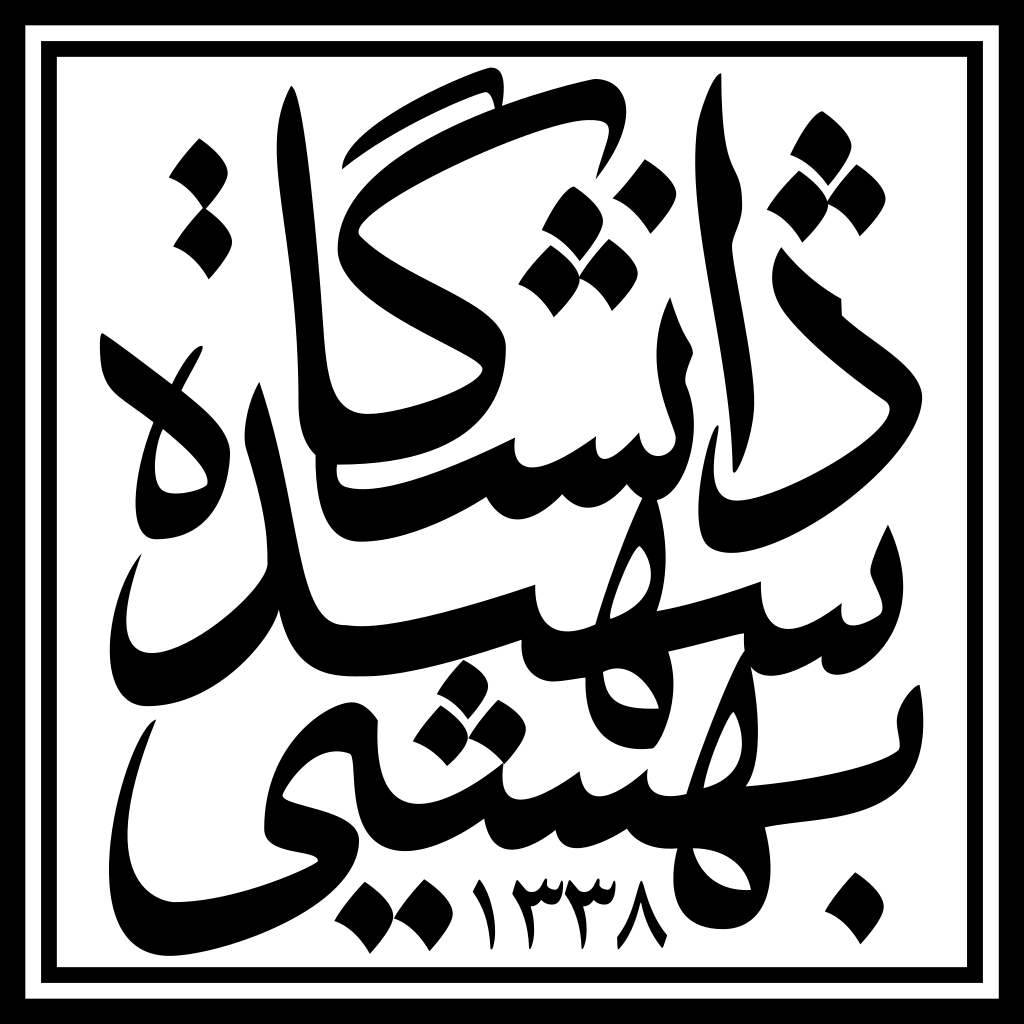
\includegraphics[height=3cm]{./logo}\\دانشگاه شهید بهشتی\\دانشکده‌ی فیزیک \par}
	\vspace{1cm}
	{
پایان‌نامه‌ ارائه شده به عنوان بخشی از ملزومات برای دریافت\\درجه‌ی کارشناسی ارشد فیزیک ذرات بنیادی و نظریه میدان‌ها 
	\par}
	\vspace{1cm}
	{\huge 
باریون‌زایی از طریق لپتون‌زایی گرمایی\\در کیهان‌شناسی‌های غیر استاندارد
	\par}
	\vspace{1cm}
	{\large
مهران دهپور
	\par}
	\vfill
	{\large
دی ۱۴۰۲
	\par}
\end{titlepage}
\restoregeometry

\chapter*{اعلامیه‌ی تالیف}
\addcontentsline{toc}{chapter}{اعلامیه‌ی تالیف}
اینجانب، مهران دهپور بدین وسیله اعلام می‌کنم این پایان‌نامه تحت عنوان «باریون‌زایی از طریق لپتون‌زایی در کیهان‌شناسی‌های غیر استاندارد» و تحقیقات ارائه شده در آن متعلق به خودم است. در مواردی که از مراجع دیگر استفاده شده است به صورت شفاف استناد شده‌اند. 
این پایان‌نامه بر اساس مقالات زیر است تهیه شده‌اند:
\par
\vspace{-0.5cm}
\lr{\footnotesize
	\begin{itemize}
		\item \bibentry{Dehpour:2023dfo}
		\item \bibentry{Dehpour:2023wyy}
	\end{itemize}
}

\chapter*{قدردانی}
\addcontentsline{toc}{chapter}{قدردانی}
این پایان‌نامه نتیجه‌ی فراگیری و یادگیری مساله‌ی عدم تقارن ماده، با راهنمایی سیامک سادات گوشه و مشاوره‌ی سعید عباسلو است. دانسته‌هایم در مورد فیزیک نوترینو را نیز مدیون یاسمن فرزان و پویا بختی هستم.  لذا از تک تک این افراد نهایت تشکر را بعمل می‌آورم.

در آخر، به طور ویژه از خانواده خود، از سحر صفری و خانواده محترم‌شان بابت همراهی اینجانب در تمامی مقاطع تحصیلی اینجانب تشکر می‌کنم. بدون اغراق، بدون کمک و حمایت آنها این پایان‌نامه بدین شکل، نمی‌توانست نگارش شود.
	
\chapter*{چکیده}
\addcontentsline{toc}{chapter}{چکیده}
{معمولا فرض بر این است که عالم در ابتدا بدون عدم تقارن ماده ایجاد شده یا عدم تقارن ماده اولیه موجود، توسط تورم شسته شده است. این بدان معناست که پس از تورم، برای هر ذره، یک پادذره منسوب وجود خواهد داشت. در این حالت باید انتظار داشته باشیم که با کاهش دما ماده و پادماده در اثر برخورد به یکدیگر نابود شوند که این به معنای عدم وجود ما نیز است. برخی با رجوع به ورای مدل استاندارد سعی بر توضیح این مساله دارند. گمان می‌رود پاسخ این سوال در دل ذره‌ی کوچکِ گریزان، نوترینو، نهان شده باشد. با معرفی و بهره‌گیری از نوترینو‌ی سترون علاوه بر ذرات مدل استاندارد، همگام با جرم‌دار کردن نوترینو توسط مکانیزم الاکلنگی، با سناریوی لپتون‌زایی می‌توان مساله‌ی عدم تقارن ماده را نیز توضیح داد. البته علی رغم موفق بودن لپتون‌زایی، ایراداتی نظیر نیاز به مقیاس جرمی بالا را هم دارا است. این می‌تواند منجر به تولید بیش از حد گراویتینو شود که در تضاد با مدل‌های ابرتقارنی است و همینطور به دلیلی انرژی غیر قابل دسترس، آن را غیر قابل آزمایش می‌کند.
	در این مطالعه، ما با رجوع به کیهان‌شناسی‌های غیر استاندارد از دو طریق برای دستیابی به لپتون‌زایی در مقیاس پایین تلاش می‌کنیم.
	اول، همانطور که می‌دانیم، مکانیک آماری مرسوم جهان شمول نیست، لذا قصد داریم بر اثرات مکانیک آماری نافزونور سالیس در کیهان اولیه تمرکز کنیم.
	دوم، از آنجایی که هیچ نشانه‌ای از همسانگردی عالم قبل از هسته‌زایی مه‌بانگ نداریم، اصل کیهان‌شناختی همسانگردی را با بهره‌گیری از متریک بیانکی نوع اول، کنار می‌گذاریم.
	ما نشان می‌دهیم که استفاده از مکانیک آماری نافزونور می‌تواند با تصحیح فراوانی تعادلی ذرات، پارامتر واپاشی و شستشو بر تولید عدم تقارن باریونی در لپتون‌زایی اثر بگذارد.
	همچنین، نتایج ما نشان می‌دهد که برای مقادیر خاصی از ناهمسانگردی، لپتون‌زایی، عدم تقارن باریونی بیشتری را نسبت به حالت استاندارد تولید کند.
	به این ترتیب، یافته‌های ما نشان می‌دهد که این رویکردها می‌توانند در دست‌یابی به لپتون‌زایی مقیاس‌های پایین کمک کنند. \par}
\vspace{0.5cm}
\noindent
کلمات کلیدی: باریون‌زایی؛ لپتون‌زایی؛ مکانیک آماری سالیس؛ متریک ناهمسانگرد بیانکی نوع اول.

\addcontentsline{toc}{chapter}{فهرست مطالب}
\tableofcontents

\addcontentsline{toc}{chapter}{فهرست جداول}
\listoftables

\addcontentsline{toc}{chapter}{فهرست تصاویر}
\listoffigures

\chapter{مقدمه}
\label{chap:introduction}
\pagenumbering{arabic}
مشاهدات کیهانی نشان از عدم تعادل بین تعداد باریون‌ها (یعنی پروتون‌ها و نوترون) و پادباریون‌ها (یعنی پادپروتون‌ها و پادنوترون‌ها) دارند. تمام موجودات قابل مشاهده نظیر ستارگان، کهکشان‌ها و ساختارها از ماده (یعنی باریون‌ها و الکترون‌ها) و نه از پادماده (یعنی پادباریون‌ها و پادالکترون‌ها) تشکیل شده است. عدم تقارن باریون عالم بصورت
\par
\vspace{-0.5cm}
{\footnotesize\begin{align}
	Y^{\rm obs}_{B} \equiv \left. \frac{n_B - \overline{n}_{B}}{s} \right|_0 = (8.73 \pm 0.35) \times 10^{-11},
\end{align}}
بیان می‌شود، که در آن {\footnotesize$n_B$}، {\footnotesize$\overline{n}_{B}$} و {\footnotesize$s$} چگالی عددی باریون، پادباریون و آنتروپی هستند و زیروند {\footnotesize$0$} بیان‌گر زمان حال است. عدم تقارن باریون عالم با روش‌های متفاوتی نظیر مشاهدات: هسته‌زایی مه‌بانگ، ناهمسانگردی‌های تابش پس‌زمینه‌ی کیهانی و ساختار بزرگ مقیاس قابل تعیین است. با توجه به مشاهدات مذکور، طبق منبع \cite{Simha:2008zj} می‌توان قید با سطح اطمینان 95\% بر عدم تقارن باریونی قرار داد.
	
اگر فرض کنیم که عالم در ابتدا بدون عدم تقارن بوجود آمده باشد، یا حتی در صورتی که عدم تقارن اولیه وجود داشته باشد با تورم کیهانی\footnote{یادآور می‌شویم که همگن بودن تابش پس‌زمینه‌ی کیهانی نیاز به وجود دوره‌ی تورم را ایجاد می‌کند \cite{Kolb:1990vq}.} شسته شده باشد، علی الاصول نیازمند یک مکانیزم مکانیکی برای تولید عدم تقارن باریون در کیهان خواهیم بود که به «باریون‌زایی» موسوم است. ساخاروف نشان‌داده که هر سناریوی باریون‌زایی باید سه شرط: نقض عدد باریونی، نقض \lr{\footnotesize C} و \lr{\footnotesize CP} و خارج از تعادل بودن دینامیک را ارضا کند \cite{Sakharov:1967dj}. نقض عدد باریونی توسط فرآیندهای اسفلرانی\footnote{یادآور می‌شویم که با توجه به ناهنجاری دستیده، می‌توان نشان داد که تغییرات جریان باریون‌ها و لپتون‌ها غیر صفر و البته برابر یکدیگرند؛ به عبارتی \lr{\footnotesize B+L} نقض می‌شود ولی \lr{\footnotesize B-L} برقرار می‌ماند. از فرآیندهای مذکور به «اسفلران» یاد می‌شود \cite{Schwartz:2014sze}.} در چارچوب مدل استاندارد برقرار است. همچنین نقض تقارن \lr{\footnotesize C} بصورت کامل توسط اندرکنش‌های ضعیف در مدل استاندارد اتفاق می‌افتد. باقی شروط ساخاروف علی رغم اینکه در مدل استاندارد وجود دارد اما برای تولید چشم‌گیر عدم تقارن کفایت نمی‌کند \cite{Gavela:1994ds,Gavela:1994dt}. بنابراین برای برطرف کردن این نیاز، مستلزم رجوع به فیزیک ورای مدل استاندارد هستیم که با معرفی منبع جدیدی برای نقض خارج از تعادل تقارن \lr{\footnotesize CP}، بتوانیم عدم تقارن کافی تولید کنیم.

مکانیزم‌های ورای مدل استاندارد بسیاری برای باریون‌زایی وجود دارد که در مراجع \cite{Elor:2022hpa,DiBari:2021fhs} بصورت اجمالی به آنها اشاره شده است. در اینجا به یکی از آنها یعنی «لپتون‌زایی گرمایی» می‌پردازیم که توسط فوکوجیتا و یاناگیدا در سال 1364 معرفی شده است \cite{Fukugita:1986hr}. ذرات جدید، نوترینوهای راست دست یا «سترون»\footnote{سترون به این اطلاق دارد که این ذره هیچ اندرکنشی جز اندرکنش گرانشی ندارد، چرا که هیچ بار الکتریکی و رنگ حمل نمی‌کند.}، که توسط مکانیزم الاکلنگی برای جرم‌دار کردن نوترینوها معرفی شده بودند \cite{Mohapatra:1980yp,Yanagida:1979as,Glashow:1979nm,Gell-Mann:1979vob,Minkowski:1977sc}؛ با جفت شدگی یوکاوا چشمه‌ی مورد نیاز برای نقض عدم تقارن \lr{\footnotesize CP} می‌تواند واقع شود.
اگرچه یکی از معایب لپتون‌زایی گرمایی نیازمندی به نوترینوی سترون با جرم بسیار زیاد است \cite{Davidson:2002qv}. این قید با مدل‌های ابرتقارن از طریق تولید مازاد گراویتینو مغایرت دارد \cite{Kawasaki:2008qe,Rychkov:2007uq,Kawasaki:1994af,Khlopov:1984pf,Weinberg:1982zq}. همچنین، این قید به لحاظ پدیدارشناسی نیز غیر قابل آزمودن می‌باشد چرا که آزمایشگاه‌های کنونی هنوز توان بررسی انرژی‌های زیر \lr{\footnotesize GeV} را دارند. اگرچه توسعه‌های نوین لپتون‌زایی مانند: در نظر گرفتن نوسان نوترینوهای سترون \cite{Pilaftsis:2003gt,Akhmedov:1998qx,Asaka:2005pn}، اندرکنش الکترومغناطیسی نوترینوهای سترون \cite{Bell:2008fm}، توانسته‌اند مقیاس جرمی نوتریوی سترون مورد نیاز را کاهش دهند؛ یکی دیگر از شاخه‌های توسعه‌ی لپتون‌زایی، در نظر گرفتن کیهان‌شناسی‌های غیر استاندارد است که مراجع \cite{sym12020300,Dutta:2018zkg,PhysRevD.90.064050} مورد توجه قرار گرفته‌اند.

در این مطالعه، بر توسعه‌ی لپتون‌زایی گرمایی با در نظر گرفتن کیهان‌شناسی‌های غیر استاندارد متمرکز می‌شویم. دو نوع کیهان‌شناسی غیر استاندارد را در نظر خواهیم گرفت: کیهان‌شناسی نافزونور که با تعمیم مکانیک آماری حاکم بر عالم حاصل می‌شود و کیهان‌شناسی ناهمسانگرد که با نادیده گرفتن اصل کیهان‌شناختی همسانگردی حاصل می‌شود. نتایج ما نشان می‌دهد که این دسته از کیهان‌شناسی‌های غیر استاندارد، توانایی کاهش مشکلات لپتون‌زایی گرمایی را دارند و می‌توانند مقیاس جرم نوترینوی راست دست یا سترون مورد نیاز را کاهش دهند.

پیکربندی این پایان‌نامه به شرح زیر تنظیم شده است. در فصل \ref{chap:neutrino}، به مرور اجمالی بر فیزیک نوترینو، در حدی که مورد نیازمان است، می‌پردازیم. در فصل \ref{chap:leptogenesis}، به بیان ایده، استخراج معادلات حاکم و ایرادات لپتون‌زایی گرمایی می‌پردازیم. در فصل \ref{chap:nonextensive}، با بعد از بررسی مکانیک آماری نافزونور و اثرات آن در کیهان‌شناسی به تعمیم لپتون‌زایی گرمایی در عالم نافزونور می‌پردازیم. در فصل \ref{chap:anisotropic}، بعد از بررسی کیهان‌شناسی ناهمسانگرد به تعمیم لپتون‌زایی گرمایی در آن می‌پردازیم. در نهایت، در فصل \ref{chap:conclusion}، پیرامون نتایج بدست آمده، بحث خواهیم کرد و چشم‌اندازی از آینده این مطالعات ارائه می‌کنیم.

\chapter{فیزیک نوترینو}
\label{chap:neutrino}
فیزیک نوترینو نمونه‌ای موفق از پیشرفت دانش فیزیک است که به واسطه‌ی تعامل بین توسعه‌های نظری و پیشرفت هنر آزمایش پیش می‌رود. نوترینوها با رفتارهایی که با انتظارات‌مان متفاوت است، همیشه ما را شگفت‌زده کرده است و امید است از این طریق بتوان فیزیک جدید را شناخت. در این فصل، ما به مرور اجمالی تاریخچه و فیزیک نوترینو از زمان پیشنهاد اولیه وجود آن تاکنون خواهیم پرداخت.

\section{مقدمه}
داستان اکتشاف نوترینو به اوایل قرن بیستم برمی‌گردد. در سال 1292، جیمز چادویک با اندازه‌گیری طیف واپاشی بتازای هسته‌های پرتوزا، با توجه به ناشناخته بودن نوترینو انتظار داشت ذرات بتای مشاهده شده تک انرژی باشند چرا که در واپاشی بتازا یک هسته به هسته‌ای سبک‌تر تبدیل شده و بدلیل جرم بالایشان ساکن می‌ماند و تنها ذرات بتا انرژی حاصل از اختلاف جرم این دو باید داشته باشد. اما نتایج آزمایش برخلاف انتظار بود و طیف انرژی پیوسته‌ای برای بتا مشاهده کرد \cite{Chadwick:262756}.
بنظر می‌رسید که قانون بقای انرژی در واپاشی بتازا نقض می‌شود تا اینکه در 1308 ولفگانگ پائولی پیشنهاد وجود ذره‌ای فرمیونی خنثی را مطرح کرد که همزمان با ذره بتا در واپاشی بتازا خلق می‌شود و انرژی گم‌شده را با خود حمل می‌کند. بدین ترتیب مجموع انرژی این ذره‌ی جدید و بتا همواره مقدار ثابتی است که به بقای انرژی احترام می‌گذارد \cite{Pauli:83282}.
پائولی نام «نوترون»، به معنای خنثی، را برای این ذره جدید پیشنهاد کرد که البته بعدها بدلیل نامگذاری نوترون برای یک باریون جدید \cite{noauthor_existence_1932}، توسط انریکو فرمی در سال 1312 حین فرمول‌بندی واپاشی بتازا، به «نوترینو» موسوم گشت که به معنای نوترون کوچک است. لازم بذکر است که نوترینو در این فرمول‌بندی جرم‌اش بسیار کوچک‌تر از جرم بتا در نظر گفته شده است \cite{fermi_versuch_1934}. لذا واپاشی بتازا را به صورت
\par
\vspace{-0.5cm}
{\footnotesize\begin{align}
	n \to p + e^- + \overline{\nu}_e,
	\label{pro:beta-decay}
\end{align}}
		بیان می‌کنیم که انتظار داریم بدلیل پایستگی عدد لپتونی، نوترینوی حاصله به طعم الکترون باشد. وو در سال 1334 با آزمایش واپاشی بتازای هسته‌ی کبالت متوجه شد تقارن پاریته نقض می‌شود \cite{Wu:1957my}، بدین ترتیب که همه‌ی ذرات بتای خروجی چپ دست بودند، بنابرین باید پادنوترینوهای شرکت کرده در این فرآیند باید راست دست باشند \cite{PhysRev.109.1015}. این آزمایش نخستین دیدگاه در مورد اندرکنش ضعیف را شکل داد که فقط با ذرات چپ دست انجام می‌شود.

پیکربندی این فصل به شرح زیر تنظیم شده است. در بخش \ref{sec:SM-neutrinos}، با ادامه بر تاریخچه‌ی اکتشاف نوترینو، دیدگاه مدل استاندارد نسبت به نوترینوها را مطرح می‌کنیم. در بخش \ref{sec:neutrino-oscillation}، به نوسان نوترینو و لزوم جرم‌دار بودن آن می‌پردازیم. در بخش \ref{sec:massive-neutrino} به مدل‌های مرسوم جرم‌دار کردن نوترینو می‌پردازیم.

\section{نوترینوها در مدل استاندارد}
\label{sec:SM-neutrinos}
امروزه نوترینو با سه طعم متفاوت که به لحاظ باردار بودن، خنثی و بدون جرم در مدل استاندارد ذرات بنیادی معرفی می‌شود. تنها اندرکنش آنها در مدل استاندارد، اندرکنش ضعیف است. این در حالی است که مشاهدات تا مدت‌ها هیچ نشانه‌ای از وجود طعم‌های مختلف را ارائه نمی‌دادند. در ادامه به داستان اکتشاف سه طعم نوترینو و ویژگی‌های مشابه و تفاوت‌هایشان خواهیم پرداخت.
\subsubsection{نوترینوی الکترون}
طبق آزمایش‌های اولیه که متوجه خنثی بودن و جرم ناچیز نوترینو شدیم، دشواری مشاهده نوترینو دور از ذهن نیست و بدین علت اولین آشکارسازی آن به بیست سال پس از پیشنهاد وجودش موکول شد. در سال 1334، رینز و کوان برای اولین بار شار پادنوترینوی منتشر شده از یک رآکتور هسته‌ای را در سایت رودخانه‌ی ساوانا در آمریکا مشاهده کردند \cite{SRS} که رینز در 1374 بدین علت نیمی از جایزه نوبل را برنده شد.
آشکارساز آن یک مخزن بزرگ پر از آب به عنوان منبع پروتون بود و بدین ترتیب با برخورد پادنوترینوهای الکترون منتشر شده از واپاشی بتازا داخل رآکتور جذب می‌شدند و با فرآیند واپاشی بتازای معکوس به صورت
\par
\vspace{-0.5cm}
{\footnotesize\begin{align}
	\overline{\nu}_e + p \to n + e^+,
	\label{pro:inverse-beta-decay}
\end{align}}
نوترون و پوزیترون تولید می‌شد. پوزیترون حاصله بلافاصله با الکترون‌های محیط برهمکنش کرده و دو فوتون آزاد می‌کند که توسط سوسوزن‌ها\footnote{مواد سوسوزن که اشکال مختلف مایع و بلور دارد، ماده‌ای است که با حرکت ذره باردار در آن، فوتون آزاد می‌کند که توسط آشکارسازهای فوتون قابل مشاهده است.} قابل تشخیص است. لازم بذکر است که نوترون‌های تولید شده نیز باید به نحوی از بین بروند تا مجددا از طریق کانال واپاشی بتازا و تولید الکترون، سیگنال ثانویه‌ای برای مشاهده نوترینو نباشند و بدین منظور از مواد جاذب نوترون نظیر گادلینیوم، که به سموم نوترون موسوم هستند، استفاده می‌کنند.
		
\subsubsection{نوترینوی میون}
طبق آزمایشات، طیف انرژی میون‌های تولید شده در واپاشی پایون همانند واپاشی بتازا که در ابتدای بخش \ref{sec:SM-neutrinos} مطرح شد، پیوسته بود که وجود نوترینوای در این اندرکنش را گواهی می‌داد. سوالی که به درستی مطرح شد این بود که آیا نوترینوی بوجود آمده در این برهمکنش با نوترینوی بوجود آمده در واپاشی بتازا یعنی فرآیند (\ref{pro:beta-decay}) یکسان است یا خیر؟ لدرمن، شوارتز و اشتاینبرگز در سال 1340 آزمایشی را در شتاب‌دهنده‌ی سنکروتون گرادیان متناوب در آزمایشگاه ملی بروکهیون آمریکا انجام دادند که وجود دو طعم مختلف نوترینو را اثبات کرد \cite{AGC} و جایزه‌ی نوبل 1366 را برای آنان به ارمغان آورد. در این آزمایش ذرات تولید شده از واپاشی پایون‌های باردار\footnote{یادآوری می‌کنیم که طبق قضیه‌ی فری واپاشی پایون خنثی به زوج‌های فوتون است \cite{PhysRev.51.125}.} را از دیوار فولادی به ضخامت حدودا 13 متر عبور دادند تا از رسیدن هر ذره‌ای جز نوترینوها به آن سوی دیوار جلوگیری کند. سپس این نوترینوها با برخورد ورقه‌های آلومینیومی ذرات باردار بوجود آمده را توسط سوسوزن‌ها مشاهده کنند. در صورتی که فقط یک نوع نوترینو وجود داشت انتظار داشتیم که مطابق
\par
\vspace{-0.5cm}
{\footnotesize\begin{align}
	\nu_{\mu} +‌ n &\to \mu^- + p,\\
	\nu_e +‌ n &\to e^- + p,
\end{align}}
به یک اندازه میون و الکترون مشاهده شود، حال آنکه فقط ذره میون رصد شد. بنابراین نتیجه گرفتند دو نوع مجزا نوترینو وجود دارد. بنابراین امروزه واپاشی پایون‌های باردار به صورت زیر بیان می‌شوند:
\par
\vspace{-0.5cm}
{\footnotesize\begin{align} 
	\pi^+ &\to \mu^+ + \nu_{\mu},\\
	\pi^- &\to \mu^- + \overline{\nu}_{\mu}.
	\label{pro:pi-decay}
\end{align}}

\subsubsection{نوترینوی تاون}
در سال 1368 برخورد دهنده‌ی بزرگ الکترون پوزیترون در سرن اعلام کرد سه طعم نوترینو با جرم کمتر از نصف جرم بوزون {\footnotesize$Z$} وجود دارد \cite{LEP}. اگر انرژی الکترون و پوزیترونی که برخورد می‌کردند بیشتر از بوزون {\footnotesize$Z$} باشد، در پی برخورد آنها، {\footnotesize$Z$} تولید می‌شود. از طرفی طبق مدل استاندارد ذرات بنیادی انتظار می‌رود که بوزون {\footnotesize$Z$} به همه‌ی فرمیون‌هایی که جرم آنها کمتر از نصف جرم‌اش باشد واپاشی می‌کند. به صورت کلی می‌توان پهنای این واپاشی را بصورت
\par
\vspace{-0.5cm}
{\footnotesize\begin{align}
	\Gamma_{Z \to f \overline{f}} = \Gamma_{\rm vis} + \Gamma_{\rm inv},
\end{align}}
نوشت که در آن
{\footnotesize\begin{align}
	\Gamma_{\rm vis} &= \sum_{l} \Gamma_{Z \to l \overline{l}} + \sum_{q \neq t} \Gamma_{Z \to q \overline{q}},\\
	\Gamma_{\rm inv} &= N_{\nu} \Gamma_{Z \to \nu \overline{\nu}},
	\label{eq:decay-width-inv}
\end{align}}
باشند. واپاشی بوزون {\footnotesize$Z$} به نوترینوها مستقیما قابل مشاهده نبود ولی با در نظر گرفتن اینکه نرخ واپاشی به طعم‌های مختلف نوترینو باهم برابر باشند می‌توان سهم واپاشی به آنها را به صورت حاصل ضرب تعداد طعم‌های نوترینو در نرخ واپاشی بوزون {\footnotesize$Z$} به آن به صورت معادله‌ی (\ref{eq:decay-width-inv}) نوشت. لذا بدین ترتیب می‌توان بدست آورد،
\par
\vspace{-0.5cm}
{\footnotesize\begin{align}
	N_{\nu} = 2.984 \pm 0.008.
\end{align}}
لازم به ذکر است که همزمان، داده‌های کیهان‌شناسی نظیر تابش پس‌زمینه‌ی کیهانی، نیز سازگاری با این نتیجه را اعلام می‌کردند که به عنوان مثال برای اطلاعات بیشتر می‌توان به مرجع \cite{Gerbino:2022nvz} مراجعه کرد.
		
در نهایت، نوترینوی تاون در سال 1378 توسط آزمایش دونات در آزمایشگاه فرمی کشف شد \cite{Fermilab}. در این آزمایش پروتون‌های پر انرژی را به تنگستن تاباندند که منجر به تولید جریانی از ذرات شد. در واپاشی‌های بعدی برخی از این ذرات به لپتون تاون واپاشی کردند که خود به خود به نوترینوی تاون واپاشی می‌کند. در نهایت با قراردادن دیواره‌های سنگین که مانع از عبور همه ذرات بجز نوترینوها می‌شود، توانستند اثرات نوترینوی تاون را آشکار کنند.
		
البته دانش‌ما نسبت به نوترینوی تاون بدلایل سطح مقطع کم، آستانه‌ی انرژی تولید بالای آن و سختی تمیز آن از سایر طعم‌های نوترینو، همچنان کم است و امید است آزمایش‌های آینده دانش‌مان را به آن زیاد کنند. برای مطالعه‌ی یبشتر در مورد نوترینوی تاون و کاوش‌های نوین این حوزه می‌توان منبع \cite{MammenAbraham:2022xoc} را مطالعه کرد.

\section{نوسان نوترینو}
\label{sec:neutrino-oscillation}
در دهه‌ی 1340 آزمایش هومستیک\footnote{لازم بذکر است که رهبری این آزمایش توسط داویس انجام شد که در ابتدا به منظور رصد واپاشی پروتون برای تست تئوری اتحاد بزرگ ساخته شد. در نهایت ایشان و کوشیبا که در آزمایش کمیوکنده فعالیت داشته بدلیل رصد نوترینوهای فرازمینی، یعنی خورشیدی و اتمسفری جایزه نوبل 1381 را از آن خود کردند.} که برای اندازه‌گیری نوترینوهای خورشیدی ساخته شده بود، تناقضی را بین نتایج و پیش‌بینی مدل استاندارد خورشید اعلام کرد \cite{PhysRevLett.20.1205}. این آزمایش تنها یک سوم نوترینوهای پیش‌بینی شده توسط مدل استاندارد خورشید را اندازه‌گیری می‌کرد. یکی از راه‌های توجیه این مشکل نوسان نورینو بود. قبول کردن نوسان نوترینو مستلزم جرم‌دار بودن آنها است که با فرض بدون جرم بودن نوترینوها در مدل استاندارد ذرات بنیادی در تناقض است.
نخستین بار در سال 1336، پونتوکوروو ایده‌ی نوسان نوترینو و پادنوترینو را مطرح کرده بود \cite{Pontecorvo:1957qd}. او پس از بروز مشکل نوترینوهای خورشیدی ایده‌اش را به صورت نوسان بین طعم‌های مختلف نوترینو فرمول‌بندی کرد \cite{Pontecorvo:1969}. به موازات آن، ماکی، ناکاگاوا و ساکاتا نیز در سال 1340 رهیافتی را برای توصیف آمیختگی نوترینوها توسعه دادند \cite{MNS}.
		در نهایت با تایید دقیق‌تر نوسان نوترینو و جرم‌دار بودن آنها توسط آزمایش‌های کمیوکنده و رصدخانه نوترینوی سادبری جایزه‌ی نوبل 1394 به کاجیتا و مک‌دونالد اهدا شد.
		
\subsection{فرمول‌بندی نوسان نوترینو}
در این بخش، فرمول‌بندی مرسوم نوسان نوترینو را برگرفته از منبع \cite{Giunti:2007ry} به طور خلاصه بیان می‌کنیم.
ایده‌ی اصلی نوسان نوترینو، یکسان نبودن ویژه حالت‌های جرم و ویژه‌حالت‌های طعم آنها است\footnote{انگیزه‌ی این گزاره این است که نوترینوها اندرکنش بسیار محدودی دارند و در حین انتشار آنها به ندرت آشکارسازی می‌شوند و به عبارتی در ترکیب خطی از حالت‌های مختلف‌اش قرار می‌گیرد. به همین علت نیز لپتون‌های باردار نوسان نمی‌کنند، چرا که مدام در حین انتشار توسط اندکنش الکترومغناطیسی در حال آشکار سازی هستند.}. در واقع اگر ویژه حالت طعم نوترینو ترکیب خطی‌ای از ویژه حالت‌های جرم آن باشد، طی تحول زمانی به ترکیب خطی متفاوتی تبدیل می‌شود. این بدین علت است که هر کدام از ویژه حالت‌های جرم که ویژه حالت‌های غیر تبهگن عملگر هامیلتونی هستند، بصورت متفاوتی در زمان تحول می‌یابند.
لذا با توجه به اینکه در لحظه‌ی نخستِ تولید نوترینو در اندکنش ضعیف جریان باردار از یک لپتون باردار، نوترینو با ویژه حالت طعم {\footnotesize$\alpha$} و تکانه‌ی {\footnotesize$\vec{p}$} مشخص شود؛ این حالت را بواسطه‌ی ماتریس یکانی {\footnotesize$U$} ترکیب خطی از ویژه حالت‌های جرم می‌توان نوشت
\par
\vspace{-0.5cm}
{\footnotesize\begin{align}
	|\nu_\alpha\rangle = \sum_{k} U^*_{\alpha k} |\nu_k\rangle,
	\label{eq:osc-1}
\end{align}}
با توجه به معادله‌ی تحول شیرودینگر می‌توان ویژه حالت جرم نوترینو را توسط هامیلتونی در گذر زمان {\footnotesize$t$} تحول داد
{\footnotesize\begin{align}
	|\nu_k(t)\rangle = e^{-iE_kt} |\nu_k\rangle,
	\label{eq:osc-2}
\end{align}}
که در آن انرژی با رابطه‌ی پاشندگی {\footnotesize$E_k = \sqrt{\vec{p}^2 + m_k^2}$} داده می‌شود.
حال با توجه به تعریف، اگر {\footnotesize$|\nu_{\alpha}(t)\rangle$} نمایانگر نوترینوای باشد که در زمان {\footnotesize$t=0$} با طعم {\footnotesize$\alpha$} خلق شده باشد؛ می‌توان با توجه به دو معادله‌ی (\ref{eq:osc-1}) و (\ref{eq:osc-2}) تحول این موجود را بصورت زیر بیان کرد
\par
\vspace{-0.5cm}
{\footnotesize\begin{align}
	|\nu_\alpha (t)\rangle = \sum_{k} U_{\alpha k} e^{-iE_k t} |\nu_k\rangle.
	\label{eq:osc-3}
\end{align}}
با توجه به وارون معادله‌ی (\ref{eq:osc-1}) می‌توان رابطه‌ی (\ref{eq:osc-3}) را که بر حسب ویژه حالت‌های جرمی بود را به ویژه حالت‌های طعم تغییر داد:
\par
\vspace{-0.5cm}
{\footnotesize\begin{align}
	|\nu_{\alpha}(t)\rangle=\sum_{\beta}\left(\sum_{k}U^*_{\alpha k} e^{-iE_kt}U_{\beta k}\right) |\nu_{\beta}\rangle.
\end{align}}
بدین ترتیب احتمال گذار از طعم {\footnotesize$\alpha$} به {\footnotesize$\beta$} را بعد از گذشت زمان {\footnotesize$t$} می‌توان بدست آورد:
{\footnotesize\begin{align}
	P_{\alpha \beta}(t) &=|\langle\nu_{\beta}|\nu_{\alpha}(t)\rangle|^2 \notag\\
	&= \sum_{j ,k} U^*_{\alpha j} U_{\beta j} U_{\alpha k} U^*_{\beta k} e^{-i(E_j - E_k)t}.
	\label{eq:transition-prob}
\end{align}}
حال با فرض فوق نسبیتی بودن نوترینو می‌توان عنوان کرد رابطه‌ی پاشندگی بصورت
{\footnotesize\begin{align}
	E_k=|\vec{p}|+\frac{m_k^2}{2|\vec{p}|},
\end{align}}
است. لذا با توجه به تعریف {\footnotesize$\Delta m_{jk}^2 \equiv m_j^2 - m_k^2$} می‌توان گفت
{\footnotesize\begin{align}
	E_k-E_j=\frac{\Delta m_{jk}^2}{2|\vec{p}|}.
	\label{eq:energy-difference}
\end{align}}
با جایگذاری رابطه‌ی (\ref{eq:energy-difference}) در رابطه‌ی (\ref{eq:transition-prob}) و با توجه به اینکه نوترینوی فوق نسبیتی تقریبا با سرعت نور منتشر می‌شود، می‌توان با تقریب {\footnotesize$t=L$} که {\footnotesize$L$} فاصله انتشار نوترینو است احتمال گذار را بطور
\par
\vspace{-0.5cm}
{\footnotesize\begin{align}
	P_{\alpha \beta}(L,|\vec{p}|) = \sum_{j ,k} U^*_{\alpha j} U_{\beta j} U_{\alpha k} U^*_{\beta k} e^{-i\frac{\Delta m_{jk}^2}{2|\vec{p}|}L}.
\end{align}}
نوشت. توجه شود که غیر صفر بودن چنین فرآیندی به منزله‌ی نقض عدد لپتونی طعم است و البته در صورتی که اختلاف جرم نوترینوها برابر صفر باشد نوسانی رخ نخواهد داد.

لازم به ذکر است که این ماتریس یکانی {\footnotesize$ََU$} به ماتریس پونتوکورو-ماکی-ناکاگاوا-ساکاتا (\lr{\footnotesize PMNS}) موسوم است. حال کلی‌ترین حالت ماتریس \lr{\footnotesize PMNS} را در صورتی که دو نوترینو داشته باشیم بصورت
\par
\vspace{-0.5cm}
{\footnotesize\begin{align}
	U=\begin{pmatrix}
		\cos\theta&\sin\theta\\
		-\sin\theta&\cos\theta
	\end{pmatrix},
	\label{eq:PMNS-2}
\end{align}}
می‌توان نوشت که تنها یک زاویه‌ی اختلاط {\footnotesize$\theta$} دارد که توسط آزمایش‌های نوسان نوترینو باید تببین شود. این فرمول‌بندی در آزمایش‌هایی که تنها دو گونه نوترینو وجود دارد مثل آزمایش‌های رآکتوری تقریب مناسبی می‌باشد ولی در صورتی که بخواهیم دقیق‌تر بیان کنیم باید با فرض سه نوترینو ماتریس \lr{\footnotesize PMNS} را بسازیم. با قرارداد مرسوم منبع \cite{PhysRevLett.53.1802} بسط ماتریس \lr{\footnotesize PMNS} با تعاریف {\footnotesize$s_{ij} \equiv \sin \theta_{ij}$} و {\footnotesize$c_{ij} \equiv \cos  \theta_{ij}$} بصورت
\par
\vspace{-0.5cm}
{\footnotesize\begin{align}
	U = 
	\begin{pmatrix}
		1&0&0\\0&c_{23}&s_{23}\\0&-s_{23}&c_{23}
	\end{pmatrix}
	\begin{pmatrix}
		c_{13}&0&s_{13}e^{-i\delta}\\0&1&0\\s_{13}e^{i \delta}&0&c_{13}
	\end{pmatrix}
	\begin{pmatrix}
		c_{12}& s_{12} & 0\\-s_{12} & c_{12} & 0 \\ 0 & 0 & 1
	\end{pmatrix},
	\label{eq:PMNS-3}
\end{align}}
نوشته می‌شود، که شامل سه زاویه‌ی اختلاط {\footnotesize$\theta_{12}$}، {\footnotesize$\theta_{13}$} و {\footnotesize$\theta_{23}$} و یک فاز {\footnotesize$\delta$} موسوم به فاز دیراک\footnote{در صورت مایورانا بودن نوترینو، دو فاز ناقض \lr{\footnotesize CP} نیز پدیدار خواهد گشت که به فاز‌های مایورانا موسوم هستند. در این مورد در معادله‌ی (\ref{eq:Majorana-phases}) صحبت خواهیم کرد.} یا فاز(های) ناقض \lr{\footnotesize CP}\footnote{دلیل اینکه این پارامتر به نقض \lr{\footnotesize CP} مرتبط شده است این است که رابطه‌ی (\ref{eq:CP-violation}) متناسب می‌شود با قسمت موهومی ماتریس \lr{\footnotesize PMNS} که تنها در صورت غیر صفر بودن پارامتر {\footnotesize$\delta$}، غیر صفر می‌شود؛ همینطور در لپتون‌زایی که طبق رابطه‌ی (\ref{eq:cp-parameter}) باید جفت‌شدگی یوکاوا موهومی باشد و در چارچوب مکانیزم الاکلنگ نوع یک، طبق رابطه‌ی (\ref{eq:Casas-Ibarra-2}) یا (\ref{eq:Casas-Ibarra-3})، این شرط زمانی فراهم می‌شود که (یا ماتریس {\footnotesize$R$} موهومی شود یا) ماتریس \lr{\footnotesize PMNS} موهومی شود که توسط فاز‌ {\footnotesize$\delta$} امکان پذیر می‌شود.} است. لازم بذکر هست که زوایای اختلاط نامبرده بترتیب بدلیل نحوه‌ی تعیین‌شان برای نخستین بار در آزمایش‌های نوترینوهای خورشیدی، رآکتوری و اتمسفری به همین نام‌ها نیز موسوم هستند. 
بطور دقیق‌تر می‌توان گفت آزمایش‌های نوسان نوترینو با توجه به چشمه‌ی نوترینوشان که انرژی و فاصله‌شان متفاوت است حساسیت‌های متفاوتی نسبت به پارامتر‌های نوسان دارند. آزمایش‌های نوترینوهای خورشیدی، حساسیت خوبی نسبت به پارامتر‌های {\footnotesize$\theta_{12}$}، {\footnotesize$\theta_{13}$} و {\footnotesize$\Delta m^2_{21}$} دارند. آزمایش‌های نوترینوهای اتمسفری حساسیت خوبی نسبت به پارامترهای {\footnotesize$\theta_{23}$}، {\footnotesize$\theta_{13}$}، {\footnotesize$\Delta m^2_{31}$} و {\footnotesize$\delta$} دارند. آزمایش‌های نوترینوهای رآکتوری حساسیت خوبی نسبت به پارامترهای {\footnotesize$\theta_{13}$} و {\footnotesize$\Delta m^2_{31}$} دارند. آزمایش‌های نوترینوهای شتاب‌دهنده‌ها حساسیت خوبی نسبت به پارامتر‌های {\footnotesize$\theta_{23}$}، {\footnotesize$\theta_{13}$}، {\footnotesize$\Delta m^2_{31}$} و {\footnotesize$\delta$} دارند.

فرمول‌بندی‌ای که بررسی کردیم برای نوسان نوترینو در خلا بود، اما اثرات ماده که باعث اندرکنش ضعیف نوترینو با مواد تشکیل دهنده اش می‌شود را بحساب نیاوردیم. چنین اثری تحت عنوان میخییو، اسمیرنوف و ولفشتاین (\lr{\footnotesize MSW}) شناخته می‌شود که در آنالیز داده‌های آزمایش‌های نوترینوهایی که طول انتشارشان زیاد و از مسیر مادی میگذرد، نقش مهمی بازی می‌کند \cite{Mikheyev:1985zog,Wolfenstein:1977ue}. این اثرات باعث تشدید نوسان شده و می‌توان بصورت نظری،‌ این اثرات را در بازتعریف زاویه‌ی اختلاط موثر و اختلاف جرم موثر نوترینو گنجاند \cite{Giunti:2007ry}.

در نهایت اشاره می‌کنیم که نوسان نوترینو میتواند همینطور عدم تقارن‌ها را نیز برایمان آشکار کنند. بدین منظور می‌توان میزان عدم تقارن \lr{\footnotesize CP} را بصورت
\par
\vspace{-0.5cm}
{\footnotesize\begin{align}
	\mathcal{A}^{\rm CP}=P_{\alpha \beta}-P_{\overline{\alpha} \overline{\beta}},
	\label{eq:CP-violation}
\end{align}}
عدم تقارن \lr{\footnotesize T} را بصورت
{\footnotesize\begin{align}
	\mathcal{A}^{\rm T}=P_{\alpha \beta}-P_{\beta \alpha},\notag\\
	\mathcal{A}^{\rm T}=P_{\overline{\alpha} \overline{\beta}}-P_{\overline{\beta} \overline{\alpha}},
\end{align}}
و عدم تقارن \lr{\footnotesize CPT} را بصورت
{\footnotesize\begin{align}
	\mathcal{A}^{\rm CPT}=P_{\alpha \beta}-P_{\overline{\beta} \overline{\alpha}},
\end{align}}
اندازه‌گیری کرد.
		
\subsection{وضعیت کنونی آزمایشگاهی نوسان  نوترینو}
آزمایش‌های کنونی نوسان نوترینو در مرجع \cite{Denton:2022een} به اختصار معرفی شده‌اند. طبق دانش بدست آمده تاکنون در مورد نوترینوها، می‌توان پارامتر‌های نوسان نوترینو را به سه زاویه‌ی آمیختگی و دو اختلاف جرم خلاصه کرد که محدوده‌ی آنها طبق آخرین تحلیل جامع\footnote{در تحلیل جامع نتایج تمام آزمایش‌های موجود توسط رهیافت‌های آماری با یکدیگر ادغام می‌شود. در ابتدای این تحلیل‌ها، عده‌ای با این نحوه‌ی تحلیل داده‌ها موافق نبودند و گمان می‌کردند تیم تحلیل‌گر ممکن است اثر پس‌زمینه‌ی آزمایش‌ها را از یکدیگر نمی‌تواند جدا کرد؛ از یک سوی دیگر قبل از اندازه‌گیری {\footnotesize$\theta_{13}$} نتایج تحلیل جامع در ابتدا نشان از غیر صفر بودن {\footnotesize$\theta_{13}$} می‌داد که با گمانه‌زنی‌های نظری مانند مرجع \cite{Harrison:2002er} در تضاد بود و این موضوع نیز باعث پذیرفته نشدن تحلیل‌های جامع بود که در نهایت با اندازه‌گیری‌های آزمایش‌های رآکتوری مشخص شد که تحلیل‌های جامع پیش‌بینی درستی انجام داده بود.} در شکل \ref{fig:NuFIT} برگرفته از نتایج گروه \lr{\footnotesize NuFIT}\footnote{لازم بذکر است که گروه‌های فعال دیگری نیز مشغول به تحلیل جامع هستند که می‌توان به نتایج آخر گروه ولنسیا \cite{deSalas:2020pgw} و گروه باری \cite{Capozzi:2021fjo} اشاره کرد که در حال حاضر تفاوت چندانی با یکدیگر ندارند.} \cite{Esteban:2020cvm} قابل ملاحظه است. اگرچه هنوز تکه‌هایی از این پازل نظیر موارد زیر باقی مانده است:
\begin{figure}
	\centering
	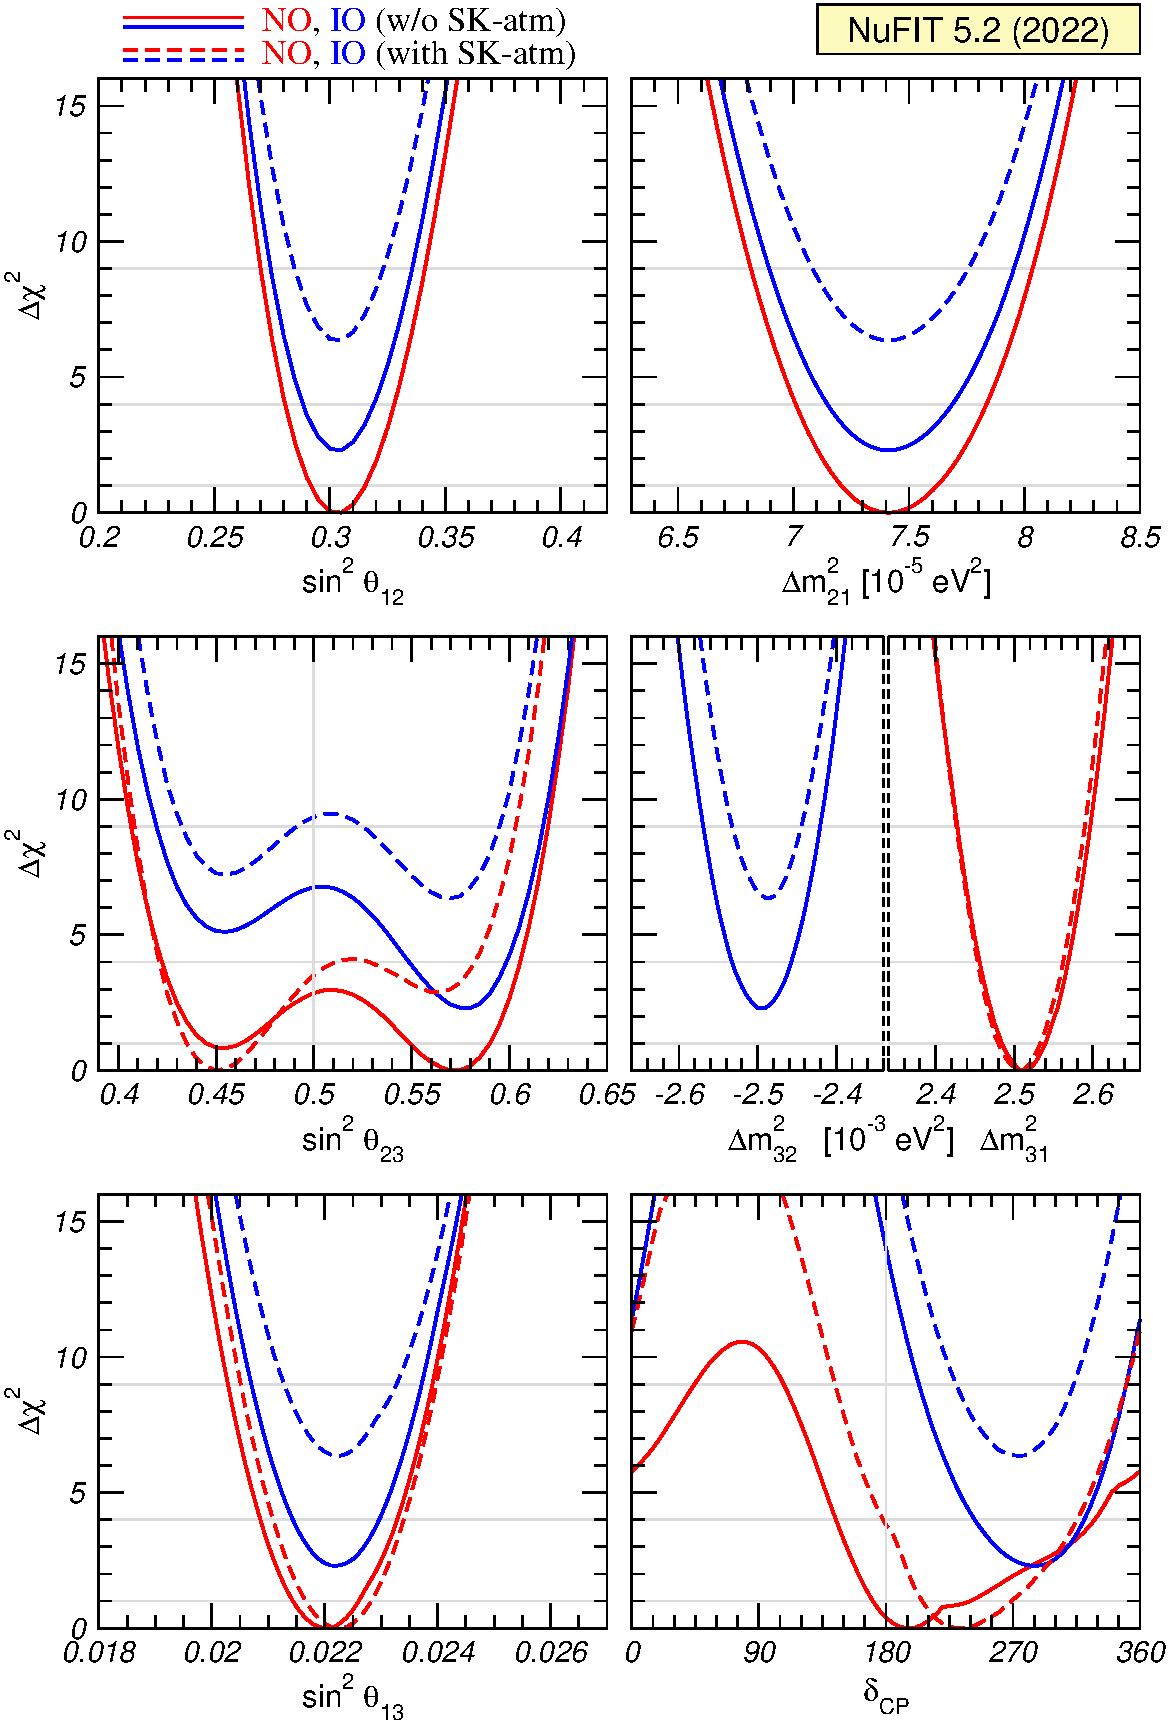
\includegraphics[width=\textwidth]{./fig-chisq-glob}
	\caption{تصاویر تک بعدی $\chi^2$ با تحلیل جامع آزمایش‌های نوسان نوترینو}
	\label{fig:NuFIT}
\end{figure}
\begin{itemize}
	\item ترتیب جرمی نوترینو:
درحالی که علامت اختلاف جرم خورشیدی، {\footnotesize$\Delta m_{\rm 21}^2=m_2^2-m_1^2$}، دانسته است، اختلاف جرم اتمسفری به صورت قدر مطلق، {\footnotesize$|\Delta m_{\rm 31}^2|=|m_3^2-m_{1,2}^2| \gg \Delta m_{\rm 21}^2$}، قابل دست‌یابی است. بنابراین در ترتیب جرمی نوترینو ابهام وجود دارد که به صورت ترتیب عادی (\lr{\footnotesize NO}) {\footnotesize$m_1^2<m_2^2<m_3^2$} است یا به صورت ترتیب وارون (\lr{\footnotesize IO}) {\footnotesize$m_3^2<m_2^2<m_1^2$}.
	\item مشخص کردن فازهای ناقض \lr{\footnotesize CP}:
فازهای ناقض \lr{\footnotesize CP} یعنی فاز دیراک {\footnotesize$\delta$} و فازهای مایورانا {\footnotesize$\alpha_{1,2}$} هنوز به خوبی اندازه‌گیری نشده‌اند. اگرچه تحلیل جامع \cite{Esteban:2020cvm} مقدار فاز دیراک {\footnotesize$\delta$} را گزارش کرده است، اما دارای خطای بزرگی است. فازهای مایورانا نیز تا زمانی که امکان آشکار کردن نوترینوهای سنگین فراهم نشود قابل اندازه‌گیری نخواهد بود \cite{Drewes:2016jae}.
	\item اکتانت {\footnotesize$\theta_{23}$}:
	با توجه به نتایج بدست آمده هنوز مشخص نیست که مقدار {\footnotesize$\theta_{23}$} از {\footnotesize$\pi/4$} بیشتر‌ است یا کمتر.
	\item جرم مطلق نوترینوها:
از آنجایی که تنها دو اختلاف جرم از طریق آزمایش‌های نوسان نوترینو قابل سنجش است، مقادیر مطلق جرم هنوز مشخص نشده است. البته آزمایش‌هایی نظیر کاترین با اندازه‌گیری مستقیم واپاشی بتازا سعی دارد جرم مطلق را اندازه‌گیری کند \cite{KATRIN:2019yun}. همینطور از طریق کیهان‌شناسی بر مجموع جرم نوترینوها قید می‌توان قرار داد \cite{Planck:2018vyg}.
\end{itemize}

لازم بذکر هست که در آزمایش‌های مختلف ناهنجاری‌هایی نیز وجود دارد که با پیش‌بینی‌ها همخوانی ندارند، یا نتایج آزمایش‌های مختلف بایکدیگر تنش دارند.
مردم در تلاش هستند تا این مشکلات را کاهش دهند و مدل درست‌تری بدست بیاورند. در این میان پیشنهادهایی نظیر وجود اندرکنش‌های غیر استاندارد با ماده \cite{Farzan:2017xzy}، وجود نوسان ناهمدوس‌زا \cite{DeRomeri:2023dht} و وجود نوترینوی سترون سبک \cite{Dasgupta:2021ies} نیز با داده‌ها بررسی می‌شوند تا وجود این مشکلات را کاهش دهند ولی در حال حاضر مدل پذیرفته شده برای نوسان نوترینو بدین صورت بود که مطرح شد.

همانند مرجع \cite{Harrison:2002er} که ذکر شد، مدل‌های نظری نیز برای تعیین ماتریس \lr{\footnotesize PMNS} همچنان در تلاش هستند ولی این تلاش‌ها بر مشاهدات و پایه‌های فیزیکی محکمی استوار نیستند، به عنوان مثالی دیگر می‌توانید مقاله‌ی \cite{Costa:2023bxw} را که تلاشی در این راستا هست را مطالعه کنید.
		
\section{نوترینوی جرم‌دار}
\label{sec:massive-neutrino}
همانطور که در بخش \ref{sec:neutrino-oscillation} شاهد بودیم، تایید اینکه نوسان نوترینو وجود دارد، منجر به جرم‌دار بودن نوترینو شد. البته به موازات جرم‌دار کردن نوترینو بعضی سعی در توجیه کوچک بودن جرم آن نیز دارند. حال مدل‌هایی برای توجیه وجود جرم کوچک نوترینو وجود دارد که می‌توانید برای اطلاعات بیشتر به مطالعات مروری \cite{deGouvea:2016qpx,Cai:2017jrq,King:2003jb} مراجعه کنید. که در این میان به رهیافت‌های مرسوم می‌خواهیم اشاره کنیم که برگرفته از منبع \cite{Giunti:2007ry} است.

\subsection{نوترینوی دیراک}
با داشتن سه نوترینوی فعال {\footnotesize$\nu_{eL}$}، {\footnotesize$\nu_{\mu L}$} و {\footnotesize$\nu_{\tau L}$} و افزودن {\footnotesize$N_s$} عدد نوترینوی راست دست «سترون»، که هیچ اندرکنشی جز گرانش ندارد، بصورت {\footnotesize$\nu_{sR}$} می‌توان جمله جرمی نوترینو را همانند دیگر فرمیون‌ها بصورت جمله جرمی دیراکی نوشت:
\par
\vspace{-0.5cm}
{\footnotesize\begin{align}
		\mathcal{L}^{\rm D}_{\rm mass}=-\sum_{s,\alpha}\overline{\nu}_{sR} M_{s\alpha}^{\rm D} \nu_{\alpha L} + {\rm H.c.},
		\label{eq:dirac-neutrino}
\end{align}}
که در آن {\footnotesize$M^{\rm D}$} ماتریس جرمی مختلط {\footnotesize$N_s\times3$}  بعدی دیراکی است. لازم بذکر است که طبق آنچه در بخش اخیر دیدیم حداقل دو نوترینوی فعال جرم دار می‌خواهیم، لذا {\footnotesize$N_s=2$} باید باشد. در صورتی که سبک‌ترین نوترینو را جرم دار بدانیم باید {\footnotesize$N_s=3$} باشد.

در این صورت می‌توان همانند دیگر فرمیون‌ها با «سازوکار هیگز» نوترینو را جرم‌دار کرد. در واقع وجود {\footnotesize$\nu_{kR}$} الزام می‌کند که در اندرکنش یوکاوا با دوتایی هیگز {\footnotesize$\phi$} و دوتایی لپتون چپ دست {\footnotesize$l$} بصورت زیر شرکت کند:
\par
\vspace{-0.5cm}
{\footnotesize\begin{align}
	\mathcal{L}^{\rm Yukawa} = \sum_{s,\alpha} Y_{\alpha s} \overline{l}_{\alpha L} \phi \nu_{sR} + {\rm H.c.},
	\label{eq:yukawa}
\end{align}}
که با شکست خود به خودی تقارن الکتروضعیف و اخذ مقدار چشمداشتی  {\footnotesize$v=\left(\sqrt{2}G_{\rm F}\right)^{-1/2} \approx 246\ {\rm GeV}$} توسط مولفه خنثی دوتایی هیگز و قطری سازی ماتریس یوکاوا، ماتریس جرمی نوترینوها که در این پایه غیر قطری هستند، بصورت زیر بدست می‌آید:
\par
\vspace{-0.5cm}
{\footnotesize\begin{align}
	M^{\rm D}_{s \alpha}=\frac{Y_{s \alpha} v}{\sqrt{2}}.
\end{align}}

\subsection{نوترینوی مایورانا}
\label{sec:majorana}
با توجه به اینکه نوترینو ذره‌ای بدون بار است، علی الاصول می‌تواند در قید زیر که به «شرط مایورانا» موسوم است قرار بگیرد
\par
\vspace{-0.5cm}
{\footnotesize\begin{align}
	\nu_R=C\overline{\nu}_L^T,
	\label{eq:majorana-cond}
\end{align}}
که در آن {\footnotesize$C$} عملگرد مزدوج بار است. این قید به معنای برابر بودن ذره و پادذره‌ی نوترینو است.

حال جمله جرمی لاگرانژی دیراک را طبق معادله‌ی (\ref{eq:dirac-neutrino}) بیاد بیاوریم، با اعمال شرط مایورانا به دو قسم راست و چپ می‌توان جمله جرمی لاگرانژی را بصورت زیر بازنویسی کرد:
\par
\vspace{-0.5cm}
{\footnotesize\begin{align}
	\mathcal{L}^L_{\rm mass}&=\frac{1}{2}\sum_{\alpha,\beta} \nu_{\alpha L}^T C^{\dagger} M_{\alpha \beta}^L \nu_{\beta L} + {\rm H.c.},\\
	\mathcal{L}^R_{\rm mass}&=\frac{1}{2}\sum_{s, s^{\prime}} \nu_{sR}^T C^{\dagger} M_{ss^{\prime}}^R \nu_{s^{\prime}R}+{\rm H.c.},
	\label{eq:majorana-neutrino}
\end{align}}
که در آن {\footnotesize$M^L$} ماترس جرمی مایورانای چپ دست مختلط {\footnotesize$3 \times 3$} بعدی و {\footnotesize$M^R$} ماتریس‌های جرمی مایورانای راست دست مختلط {\footnotesize$N_s\times N_s$}‌ بعدی هستند.

افزودن جمله جرمی مایورانا باعث می‌شود تحت تبدیل {\footnotesize${\rm U}(1)$}
لاگرانژی ناوردا نماند؛ به عنوان مثال برای یکی از جملات جرمی مایورانا منسوب به چپ دست اگر تبدیل {\footnotesize$\nu_L \to e^{i\phi} \nu_L$} اعمال گردد، لاگرانژی به فرم زیر تبدیل می‌شود:
\par
\vspace{-0.5cm}
{\footnotesize\begin{align}
	\overline{\nu}_L^C M^L \nu_L \to e^{-2i\phi}\left(\overline{\nu}_L^C M^L \nu_L\right),
	\label{eq:Majorana-lepton-num-violation}
\end{align}}
لذا عدد لپتونی کل و طعم نقض می‌شوند.
به عبارتی آزادی موجود اخیر را از دست داده‌ایم که منجر به ظاهر شدن دو فاز ناقض \lr{\footnotesize CP} دیگر تحت عناوین فازهای مایورانا در ماتریس اختلاط \lr{\footnotesize PMNS} می‌شود که بصورت زیر در معادله‌ی (\ref{eq:PMNS-3}) ضرب می‌شود
\par
\vspace{-0.5cm}
{\footnotesize\begin{align}
	\begin{pmatrix}
		1&0&0\\
		0&e^{i\lambda_{21}}&0\\
		0&0&e^{i\lambda_{31}}
	\end{pmatrix}.
	\label{eq:Majorana-phases}
\end{align}}

\subsection{نوترینوی دیراک-مایورانا}
با در نظر گرفتن یک مدل هیبریدی، فرض می‌کنیم نوترینو شامل لاگرانژی‌های جرم دیراک (\ref{eq:dirac-neutrino}) و مایورانا (\ref{eq:majorana-neutrino}) باشد، لذا جمله جرمی لاگرانژی برای نوترینو بصورت زیر نوشته می‌شود
\par
\vspace{-0.5cm}
{\footnotesize\begin{align}
	\mathcal{L}^{\rm D+M}_{\rm mass}=\mathcal{L}^{\rm D}_{\rm mass}+\mathcal{L}^{L}_{\rm mass}+\mathcal{L}^{R}_{\rm mass}.
\end{align}}
با تعریف {\footnotesize$N_L\equiv\begin{pmatrix}\nu_L&\nu_R^C\end{pmatrix}^T$} که در آن {\footnotesize$\nu_R^C \equiv \begin{pmatrix}\nu_{s_1 R}^C & \dots & \nu_{s_{{N_s}}R}^C\end{pmatrix}^T$} باشد، می‌توان جمله جرمی لاگرانژی بدست آمده را بصورت
\par
\vspace{-0.5cm}
{\footnotesize\begin{align}
	\mathcal{L}^{\rm D+M}_{\rm mass}=\frac{1}{2} N_L^T C^{\dagger}
	\begin{pmatrix}
		M^L&\left(M^{\rm D}\right)^T\\
		M^{\rm D}&M^R
	\end{pmatrix}
	N_L+{\rm H.c.},
	\label{eq:hybrid-mass-term}
\end{align}}
نوشت. 
				
حال با تعریف یک ماتریس یکانی {\footnotesize$V$} بطوری که رابطه‌ی {\footnotesize$N_L=V n_L$} برقرار باشد که در آن میدان‌های جرم‌دار نوترینو بصورت {\footnotesize$n_L=\begin{pmatrix}\nu_{1L}& \dots & \nu_{NL}\end{pmatrix}^T$} است؛ ماتریس جرمی قطری-بلوکی شده را می‌توان بدست آورد بطوری که شامل بلوک ماترس قطری نوترینوهای فعال و بلوک ماتریس قطری نوترینوهای سترون بصورت:
\par
\vspace{-0.5cm}
{\footnotesize\begin{align}
	\begin{pmatrix}
		m&0\\
		0&M
	\end{pmatrix}=V
	\begin{pmatrix}
		M^L&\left(M^{\rm D}\right)^T\\
		M^{\rm D}&M^R
	\end{pmatrix}
	V^T,
\end{align}}
می‌شود.

\subsubsection{سازوکار الاکلنگی نوع-۱}
\label{sec:seesaw}
در لاگرانژی جرمی هیبریدی دیراک-مایورانا (\ref{eq:hybrid-mass-term})، با انتخاب
{\footnotesize\begin{align}
		M^{\rm D} \ll M^R, \quad M^L=0,
\end{align}}
و ماریس یکانی {\footnotesize$V$} بصورت
{\footnotesize\begin{align}
	V=\begin{pmatrix}
		I&\left[\left(M^{R}\right)^{-1} M^{{\rm D}^T}\right]^{\dagger}\\
		-\left(M^{R}\right)^{-1} M^{\rm D}&I
	\end{pmatrix}
	\begin{pmatrix}
		iI&0\\
		0&I
	\end{pmatrix},
\end{align}}
ماتریس جرمی برای نوترینوهای فعال و سنگین، بترتیب بصورت
{\footnotesize\begin{align}
	m&\simeq -\left(M^D\right)^T \left(M^R\right)^{-1} M^D ,\\
	M&\simeq M^R
\end{align}}
بدست می‌آیند.
بدین تریتیب می‌توان دید که بدون اینکه ثابت جفت‌شدگی یوکاوا خیلی کوچک شود، با انتخاب جرم‌های بسیار بزرگ برای {\footnotesize$M^R$} جرم نوترینوهای فعال بطور خودکار کوچک می‌شود. به همین دلیل نیز این مکانیزم به «الاکلنگ» موسوم شده است.

\subsubsection{پارامتریزه کردن کازاس-ایبارا}
در چارچوب سازوکار الاکلنگی نوع-۱، به دلیل مقاصدی نظیر اسکن ساده‌تر فضای پارامتر، ماتریس ثوابت جفت‌شدگی یوکاوا را به روش کازاس-ایبارا می‌توان پارامتریزه کرد \cite{Casas:2001sr}. اثبات این پارامتریزه کردن در مرجع \cite{Lopez-Pavon:2015cga} شرح داده شده است. با فرض {\footnotesize$N_s=2$}، ماتریس یوکاوا در پایه‌های جرمی بصورت
\par
\vspace{-0.5cm}
{\footnotesize\begin{align}
	y=-iU\sqrt{D_m} P_{NO} R^T(z) \sqrt{D_M} \frac{\sqrt{2}}{v},
	\label{eq:Casas-Ibarra-2}
\end{align}}
می‌شود که {\footnotesize$D_m$} ماتریس قطری جرمی نوترینوهای فعال، {\footnotesize$D_M$} ماتریس قطری جرمی نوترینوهای سترون و {\footnotesize$P_{NO}$} ماتریس مربوط به ترتیب جرمی نوترینو که برای دو حالت ترتیب جرمی عادی و وارون بصورت
\par
\vspace{-0.5cm}
{\footnotesize\begin{align}
	P_{NH}=\begin{pmatrix}
		0&0\\
		1&0\\
		0&1
	\end{pmatrix}, \quad
	P_{IH}=\begin{pmatrix}
		1&0\\
		0&1\\
		0&0
	\end{pmatrix}
\end{align}}
است و {\footnotesize$R(z)$}، یک ماتریس مختلط متعامد دو بعدی است که با یک پارامتر {\footnotesize$z=x+iy$} می‌توان ساخت. با فرض {\footnotesize$N_s=3$} نیز می‌توان به همین منوال نوشت
\par
\vspace{-0.5cm}
{\footnotesize\begin{align}
	y=-iU\sqrt{D_m} R^T(z_1,z_2,z_3) \sqrt{D_M} \frac{\sqrt{2}}{v},
	\label{eq:Casas-Ibarra-3}
\end{align}}
که در آن {\footnotesize$R(z_1,z_2,z_3)$} یک ماتریس مختلط متعامد سه بعدی خواهد شد که با سه پارامتر {\footnotesize$z_i=x_i+iy_i$} می‌توان ساخت.
				
\subsection{وضعیت کنونی آزمایشگاهی جرم نوترینو}
اساسا اینکه به طور آزمایشگاهی تعیین کنیم که نوترینو دیراک یا مایورانا است به جستجوی جفت-واپاشی بتازای بدون نوترینو ($0\nu \beta \beta$) می‌انجامد که واپاشی یک هسته {\footnotesize$\mathcal{N}$} با عدد جرمی {\footnotesize$A$} و عدد اتمی {\footnotesize$Z$} بصورت زیر رخ می‌دهد
\par
\vspace{-0.5cm}
{\footnotesize\begin{align}
	\mathcal{N}(A,Z)\to\mathcal{N}(A,Z+2)+2e^-,
\end{align}}
که به طور تقریبا همزمان دو الکترون مشاهده می‌شود و عدد لپتونی دو واحد نقض می‌شود که منطبق با معادله‌ی (\ref{eq:Majorana-lepton-num-violation}) است. به عبارتی دیگر این رخداد در صورت مشاهده شدن تایید می‌کند که نوترینو همان پادذره خودش است و تمایزی بین آنها وجود ندارد، چرا که طبق
\par
\vspace{-0.5cm}
{\footnotesize\begin{align}
	n_1 \to p_1+ e^-_1 + \nu,\notag\\
	n_2 + \nu \to p_2 + e^-_2,
\end{align}}
باید نوترینوی تولید شده توسط واپاشی بتازای اول، توسط نوترون دیگر جذب شده و وارون واپاشی بتازا رخ دهد. چنین رخدادی هنوز مشاهده نشده و آزمایش‌های زیادی در حال کاوش برای چنین رخدادی هستند که برای اطلاع از آخرین وضعیت‌شان می‌توان به مرجع \cite{Dolinski:2019nrj} مراجعه کرد.

\chapter{لپتون‌زایی گرمایی}
\label{chap:leptogenesis}
لپتون‌زایی یک دسته از سناریوهای باریون‌زایی است که عدم تقارن باریونی از عدم تقارن لپتونی توسط واپاشی ذرات سنگین یعنی نوترینوهای سترون نشات می‌گیرد. ما انگیزه‌های لپتون‌زایی را مطرح خواهیم کرد. ما به مرور سازوکار ابتدایی آن یعنی لپتون‌زایی گرمایی\footnote{لپتون‌زایی گرمایی به لپتون‌زایی استاندارد یا وانیلی نیز موسوم است. وانیلی نامیدن آن به این اتلاق دارد که از اثرات طعم صرف نظر شده است.} خواهیم پرداخت.
\section{مقدمه}
ایده‌ای اصلی این سناریو بدین صورت است که حداقل دو نوترینوی راست دست مایورانا، که در بخش \ref{sec:majorana} معرفی شد، به مدل استاندارد افزوده می‌شوند که با شرکت در مکانیزم الاکلنگی نوع-۱ مساله‌ی کوچک بودن جرم نوترینوهای فعال را حل کند، همانطور که در بخش \ref{sec:seesaw} بیان شد. این نوترینوهای راست دست بعد از تولید آنها در جهان اولیه به روش گرمایی\footnote{یعنی در جهان اولیه با سعی بر رسیدن به میزان تعادل گرمایی تولید می‌شود.}، با توجه به اینکه در اندرکنش یوکاوا با لاگرانژی (\ref{eq:Yukawa-mass-bases}) شرکت دارند از طریق این کانال می‌توانند واپاشی کنند. این واپاشی در مقایسه با نرخ هابل در دما‌های بالا، خارج از تعادل نیز است. ضمنا توجه شود که تا دمای جرم نوترینوی راست دست {\footnotesize$M_k$}، فرآیند‌های رفت و برگشت
\par
\vspace{-0.5cm}
{\footnotesize\begin{align}
	N_k \rightleftarrows \overline{\phi} l_{jL},
	\label{eq:decay}\\
	N_k \rightleftarrows \phi \overline{l}_{jL},
	\label{eq:decay-anti}
\end{align}}
انجام می‌شوند ولی بعد از آن دما، تنها در یک جهت، یعنی از چپ به راست، انجام می‌شوند. حال در صورتی که نرخ واپاشی دو فرآیند مذکور یکسان نباشد، می‌تواند به نقض تقارن \lr{\footnotesize CP} منجر شود، چرا که این دو فرآیند تحت تبدیل \lr{\footnotesize CP} به یکدیگر تبدیل می‌شوند، که خواهیم دید توسط تصحیحات حلقه این امکان وجود دارد. بنابراین علی الاصول دو مورد از شرایط ساخاروف می‌تواند ارضا شود.
سپس از طریق  فرآیندهای اسفلرانی با ارضا کردن شرط دیگر ساخاروف، عدم تقارن باریونی را می‌توان توجیه کرد.

برای بیان این فصل اگرچه مرجع اصلی کار \cite{Fukugita:1986hr} بوده ولی مرجع \cite{Luty:1992un} را در نظر می‌گیریم که نخستین‌بار بصورت سیستماتیک لپتون‌زایی را مطالعه کرده است.
در ادامه‌ی این فصل، ما فرض می‌کنیم سه نوترینوی سترون وجود دارد که برای سادگی تنها یکی از آنها از طریق کانال هیگز واپاشی می‌کند. 

پیکربندی این فصل به شرح زیر تنظیم شده است. در بخش \ref{sec:decay-rates}، نرخ واپاشی نوترینوی سترون را در حد درختی بدست می‌آوریم. در بخش \ref{sec:CP}، با محاسبه‌ی نرخ واپاشی نوترینوی سترون با تصحیحات حلقه به نقض شدن تقارن \lr{\footnotesize CP} می‌پردازیم. در بخش \ref{sec:Boltzmann} استخراج معادلات تحول نوترینوی سترون و عدم تقارن لپتونی می‌پردازیم. در بخش \ref{sec:baryon-asymmetry} به ارتباط عدم تقارن لپتونی و عدم تقارن باریونی می‌پردازیم.

\section{واپاشی نوترینوی راست دست}
\label{sec:decay-rates}
برای کمی کردن این سناریو، در قدم نخست، به محاسبه‌ی نرخ واپاشی‌های مذکور (\ref{eq:decay}) و (\ref{eq:decay-anti}) در سطح درختی، طبق نمودارهای زیر که در آن {\footnotesize$q=p-p'$} است، می‌پردازیم.
\par
\vspace{-0.5cm}
{\footnotesize\begin{equation}
	\parbox{35mm}{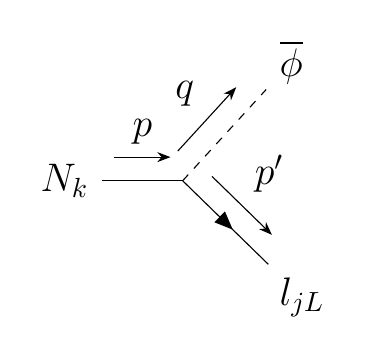
\begin{tikzpicture}
			\begin{feynman}
				\vertex (a) {\(N_k\)};
				\vertex [right=of a](b);
				\vertex [above right= of b](c) {\(\overline{\phi}\)};
				\vertex [below right=of b](d) {\(l_{jL}\)};
				
				\diagram* {
					(a) -- [momentum=\(p\)](b),
					(b) -- [momentum=\(q\),scalar] (c),
					(b) -- [momentum=\(p'\),fermion] (d),
				};
			\end{feynman}
	\end{tikzpicture}}, \quad
	\parbox{35mm}{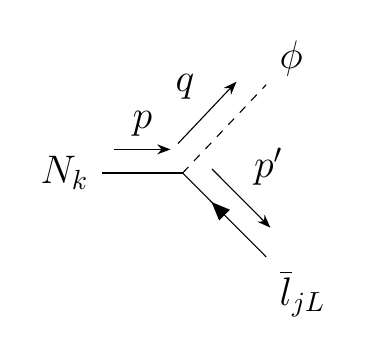
\begin{tikzpicture}
			\begin{feynman}
				\vertex (a) {\(N_k\)};
				\vertex [right=of a](b);
				\vertex [above right= of b](c) {\(\phi\)};
				\vertex [below right=of b](d) {\(\overline{l}_{jL}\)};
				
				\diagram* {
					(a) -- [momentum=\(p\)](b),
					(b) -- [momentum=\(q\),scalar] (c),
					(b) -- [momentum=\(p'\),anti fermion] (d),
				};
			\end{feynman}
	\end{tikzpicture}}.
	\label{eq:decay-tree-level}
\end{equation}}

برای فرآیند {\footnotesize$N_k \to \overline{\phi} l_{jL}$}، با توجه به قوائد فاینمن مربوطه که در پیوست‌های \ref{appendix:Dirac} و \ref{appendix:Majorana} مرور شده است، می‌توان عنصر ماتریس را بصورت
\par
\vspace{-0.5cm}
{\footnotesize\begin{align}
	i\mathcal{M}&=\overline{u}_j \left(-i y_{jk} P_R\right) u^c_k \notag \\
	&=\overline{u}_j \left(-i y_{jk} P_R\right) C \overline{u}^T_k,
	\label{eq:tree-level-M}
\end{align}}
نوشت. بنابراین دامنه مورد نظر، مطلوب است با
{\footnotesize\begin{align}
	|\mathcal{M}|^2&=\overline{u}_j \left(-i y_{jk} P_R\right) C \overline{u}^T_k \left[\overline{u}_j \left(-i y_{jk} P_R\right) C \overline{u}^T_k\right]^{\dagger} \notag\\
	&=\overline{u}_j (-i y_{jk} P_R) C \overline{u}^T_k (i y^*_{jk})(-u_k^T C^{\dagger}P_L u_j)\notag\\
	&=-(y^*_{jk} y_{jk}) \overline{u}_j P_R C \overline{u}_k^T u_k^T C^{\dagger} P_L u_j.
\end{align}}
بدین ترتیب می‌توان دامنه‌ی واپاشی را با میانگین‌گیری روی اسپین اولیه و جمع روی اسپین نهایی نوشت
{\footnotesize\begin{align}
	\langle|\mathcal{M}|^2\rangle=-\left(y^*_{jk} y_{jk}\right) P_R C \left[\frac{1}{2}\sum_{s}u_k \overline{u}_k\right]^T C^{\dagger} P_L \sum_{s'} u_j \overline{u}_j,
\end{align}}
که با توجه به بدون جرم بودن فرمیون‌ها و هیگز در کیهان اولیه می‌توان نوشت
{\footnotesize\begin{align}
	\langle|\mathcal{M}|^2\rangle&=-\frac{\left(y^*_{jk} y_{jk}\right)}{2} {\rm tr} \left[P_R\left(-\slashed{p}+M_k\right)P_L \slashed{p'}\right]\notag\\
	&=\frac{1}{2} \left(y^*_{jk} y_{jk}\right) {\rm tr}\left[P_R \slashed{p} \slashed{p'}\right]\notag\\
	&=\left(y^*_{jk} y_{jk}\right)\left(p \cdot p'\right).
	\label{eq:avraged-amplitude-lepton}
\end{align}}
حال سراغ شرایط سینماتیکی در چارچوب مرکز جرم می‌رویم. چهار تکانه‌های ذرات که طبق آنچه در نمودار (\ref{eq:decay-tree-level}) نام‌گذاری شده‌اند، برابر هستند با
\par
\vspace{-0.5cm}
{\footnotesize\begin{align}
	p=(M_k,\vec{0}), \quad p'=(M_k/2, -\vec{q}),\quad q=(M_k/2,\vec{q}).
	\label{eq:kinematic}
\end{align}}
لذا می‌توان نوشت
{\footnotesize\begin{align}
	|\vec{q}|=M_k/2, \quad
	p \cdot p' = p \cdot q = p' \cdot q = M_k^2/2.
	\label{eq:kinematicf}
\end{align}}
بنابراین با جایگذاری شرایط سینماتیکی (\ref{eq:kinematicf}) در دامنه واپاشی میانگین‌گیری شده (\ref{eq:avraged-amplitude-lepton}) می‌توان بدست آورد
{\footnotesize\begin{align}
	\langle|\mathcal{M}|^2\rangle=\frac{M_k^2}{2}(y^*_{jk} y_{jk}),
\end{align}}
با جمع روی لپتون‌های خروجی {\footnotesize$j$}\footnote{برای در نظر گرفتن اثر طعم نباید روی {\footnotesize$j$} جمع زد.} می‌توان نوشت
{\footnotesize\begin{align}
	\langle|\mathcal{M}|^2\rangle=\frac{M_k^2}{2}\left(y^{\dagger}y\right)_{kk}.
	\label{eq:avraged-amplitude-leptonf}
\end{align}}
حال، با توجه به رابطه‌ی نرخ واپاشی با عنصر ماتریس، در مرکز جرم
{\footnotesize\begin{align}
	\Gamma=\frac{|\vec{q}|}{8 \pi E_{\rm CM}^2} \langle|\mathcal{M}|^2\rangle,
	\label{eq:decay-rate-matrix-element}
\end{align}}
که در آن {\footnotesize$\vec{q}$} ‌‌‌‌تکانه‌ی یکی از ذرات خروجی و {\footnotesize$E_{\rm CM}$} انرژی مرکز جرم است. با توجه به دوتایی بودن خروجی‌های واپاشی (\ref{eq:decay-tree-level})، می‌توان نرخ واپاشی کل را بصورت
\par
\vspace{-0.5cm}
{\footnotesize\begin{align}
	\Gamma = 2 \times \frac{|\vec{q}|}{8 \pi E^2} \langle|\mathcal{M}|^2\rangle,
\end{align}}
حساب کرد. حال با جایگذاری شرایط سینماتیکی مذکور در معادله‌ی (\ref{eq:kinematicf})، {\footnotesize$E_{\rm CM}=M_k$} و عنصر ماتریس بدست آمده در معادله‌ی (\ref{eq:avraged-amplitude-leptonf}) می‌توان گفت
\par
\vspace{-0.5cm}
{\footnotesize\begin{align}
	\Gamma_k =\frac{M_k}{16 \pi} \left(y^{\dagger} y\right)_{kk}.
	\label{eq:decay-rate-lepton}
\end{align}}

به همین ترتیب می‌توان برای فرآیند {\footnotesize$N_k \to \phi \overline{l}_{jL}$} ‌‌می‌توان عنصر ماتریس را حساب کرد
{\footnotesize\begin{align}
	i\overline{\mathcal{M}}&=\left(u_k^c\right)^T \left(-i y^*_{jk} C^{\dagger} P_L\right) v_j,\notag\\
	&=i y_{jk}^* \overline{u}_k P_L v_j.
	\label{eq:matrix-element-anti-fermion}
\end{align}}
بنابراین دامنه همانند مورد قبل برابر می‌شود با
{\footnotesize\begin{align}
	|\overline{\mathcal{M}}|^2&=-i y_{jk}^* \overline{u}_k P_L v_j \left[-i y_{jk}^* \overline{u}_k P_L v_j\right]^{\dagger},\notag\\
	&=\left(y_{jk}^* y_jk\right) \overline{u}_k P_L v_j \overline{v}_j P_R u_k,
\end{align}}
سپس با میانگین‌گیری روی درجات آزادی آن می‌شود نوشت
{\footnotesize\begin{align}
	\langle|\overline{\mathcal{M}}|^2\rangle&=\left(y_{jk}^* y_{jk}\right) P_L \sum_{s'} v_j \overline{v}_j P_R \frac{1}{2} \sum_{s} u_k \overline{u}_k P_L\notag\\
	&=\frac{\left(y_{jk}^2 y_{jk}\right)}{2} {\rm tr}\left[P_L \slashed{p'} P_R (\slashed{p}+M_k)\right]\notag\\
	&=\frac{1}{2}\left(y_{jk}^* y_{jk}\right) {\rm tr}\left[P_L\slashed{p'}\slashed{p}\right]\notag\\
	&=\left(y_{jk}^* y_{jk}\right) \left(p \cdot p'\right).
	\label{eq:avraged-amplitude-anti-lepton}
\end{align}}
می‌توان دید که رابطه‌ی بدست آمده، دقیقا نظیر رابطه‌ی متناظر با فرآیند {\footnotesize$N_k \to \overline{\phi} l_{jL}$} یعنی رابطه‌ی (\ref{eq:avraged-amplitude-lepton}) است. بنابراین با اعمال همان شرابط سینماتیکی (\ref{eq:kinematicf}) و جایگذاری در رابطه‌ی نرخ واپاشی در مرکز جرم (\ref{eq:decay-rate-matrix-element}) با احتساب دوتایی بودن خروجی‌های واپاشی، دامنه واپاشی بدست می‌آید
\par
\vspace{-0.5cm}
{\footnotesize\begin{align}
	\overline{\Gamma}_k =\frac{M_k}{16 \pi} \left(y^{\dagger} y\right)_{kk}.
	\label{eq:decay-rate-anti-lepton}
\end{align}}

با توجه به نرخ‌های واپاشی بدست آمده در روابط (\ref{eq:decay-rate-lepton}) و (\ref{eq:decay-rate-anti-lepton})، برای مورد ساده‌تری که تنها یکی از نوترینوهای راست دست واپاشی کند خواهیم داشت
\par
\vspace{-0.5cm}
{\footnotesize\begin{align}
	\Gamma_1=\overline{\Gamma}_1 =\frac{M_1}{16 \pi} \left(y^{\dagger} y\right)_{11},
	\label{eq:decay-rate}
\end{align}}
که با نتیجه‌ی بدست آمده در مرجع \cite{Luty:1992un} توافق دارد.

حال با نوشتن نرخ واپاشی  موثر (درچارچوب آزمایشگاه) بصورت
{\footnotesize\begin{align}
		\Gamma(\vec{p})=\frac{M}{E(\vec{p})}\Gamma,
\end{align}}
میانگین گرمایی نرخ واپاشی‌ها را می‌توان بصورت
{\footnotesize\begin{align}
	\langle\Gamma_1(\vec{p})\rangle=\langle\overline{\Gamma}_1(\vec{p})\rangle=\langle\frac{M_1}{E(\vec{p})}\rangle\frac{M_1}{16 \pi} \left(y^{\dagger} y\right)_{11},
	\label{eq:average-decay-rate}
\end{align}}
نوشت، که در آن {\footnotesize$\langle\dots\rangle$} نماد میانگین‌گیری گرمایی روی تابع توزیع ماکسول-بولتزمان هست. بنابراین می‌توان با تعریف {\footnotesize$\beta \equiv 1/T$} بصورت زیر محاسبه کرد
\par
\vspace{-0.5cm}
{\footnotesize\begin{align}
	\langle\Gamma_1(\vec{p})\rangle=\langle\overline{\Gamma}_1(\vec{p})\rangle=
	\frac{M_1 \int_{0}^{\infty} \frac{dp\ p^2}{E(\vec{p})} \exp(-\beta E(\vec{p}))}{\int_{0}^{\infty}dp\ p^2 \exp(-\beta E(\vec{p}))}
	\frac{M_1}{16 \pi} \left(y^{\dagger} y\right)_{11}.
\end{align}}
با توجه به مرجع \cite{Kolb:1979qa} می‌توان عبارت بدست آمده را بصورت
{\footnotesize\begin{align}
	\langle\Gamma_1\rangle=\langle\overline{\Gamma}_1\rangle= \frac{K_1(z)}{K_2(z)} \frac{M_1}{16 \pi} \left(y^{\dagger} y\right)_{11},
	\label{eq:avaraged-decay-rate}
\end{align}}
نوشت، که در آن {\footnotesize$z=M_1/T$} و {\footnotesize$K_n(z)$} تابع بسل تعمیم یافته‌ی نوع دوم مربته‌ی {\footnotesize$n$} است.

\section{شکست تقارن \lr{\footnotesize CP}}
\label{sec:CP}
حال برای بیان میزان عدم تقارن \lr{\footnotesize CP}، پارامتر \lr{\footnotesize CP} را بصورت
{\footnotesize\begin{align}
	\epsilon=\frac{\Gamma - \overline{\Gamma}}{\Gamma + \overline{\Gamma}},
	\label{eq:cp-parameter-def}
\end{align}}
تعریف می‌کنیم. در حد درختی با توجه به روابط (\ref{eq:decay-rate-lepton}) و (\ref{eq:decay-rate-anti-lepton}) نرخ‌های واپاشی با یکدیگر برابرند لذا  باید به محاسبه‌ی تصحیحات حلقه بپردازیم. این موضوع را با محاسبه‌ی سرانگشتی نیز می‌توان متوجه شد. چنانچه نرخ واپاشی قابل بیان بصورت
\par
\vspace{-0.5cm}
{\footnotesize\begin{equation}
	\Gamma = \int \left\vert
	\parbox{20mm}{\begin{tikzpicture}
			\begin{feynman}[small]
				\vertex (a);
				\vertex [right=of a](b);
				\vertex [above right= of b](c);
				\vertex [below right=of b](d);
				
				\diagram* {
					(a) -- (b),
					(b) -- [scalar] (c),
					(b) -- [fermion] (d),
				};
			\end{feynman}
	\end{tikzpicture}}
	+
	\parbox{20mm}{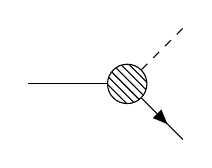
\begin{tikzpicture}
			\begin{feynman}[small]
				\vertex (a);
				\node [blob,right=of a](b);
				\vertex [above right= of b](c);
				\vertex [below right=of b](d);
				
				\diagram* {
					(a) -- (b),
					(b) -- [scalar] (c),
					(b) -- [fermion] (d),
				};
			\end{feynman}
	\end{tikzpicture}}
	+ \dots
	\right\vert^2,
\end{equation}}
است که تا تقریب 1-حلقه بدست می‌آید
{\footnotesize\begin{equation}
	\Gamma= \int \left\vert
	\parbox{20mm}{\begin{tikzpicture}
			\begin{feynman}[small]
				\vertex (a);
				\vertex [right=of a](b);
				\vertex [above right= of b](c);
				\vertex [below right=of b](d);
				
				\diagram* {
					(a) -- (b),
					(b) -- [scalar] (c),
					(b) -- [fermion] (d),
				};
			\end{feynman}
	\end{tikzpicture}}
	\right\vert^2
	+
	\left[
	\left(
	\parbox{20mm}{\begin{tikzpicture}
			\begin{feynman}[small]
				\vertex (a);
				\vertex [right=of a](b);
				\vertex [above right= of b](c);
				\vertex [below right=of b](d);
				
				\diagram* {
					(a) -- (b),
					(b) -- [scalar] (c),
					(b) -- [fermion] (d),
				};
			\end{feynman}
	\end{tikzpicture}}
	\right)^{\dagger}
	\left(
	\parbox{20mm}{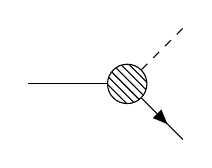
\begin{tikzpicture}
			\begin{feynman}[small]
				\vertex (a);
				\node [blob,right=of a](b);
				\vertex [above right= of b](c);
				\vertex [below right=of b](d);
				
				\diagram* {
					(a) -- (b),
					(b) -- [scalar] (c),
					(b) -- [fermion] (d),
				};
			\end{feynman}
	\end{tikzpicture}}
	\right)
	+
	{\rm H.c.}\right],
\end{equation}}
که معادل
{\footnotesize\begin{align}
	\Gamma=|y_{jk}|^2 I_{\rm tree} + y^*_{jk} y_{jm} y_{nm} y^*_{nk} I_{\rm loop} + y_{jk} y^*_{jm} y^*_{nm} y_{nk} I^*_{\rm loop},
\end{align}}
است؛ که در آن {\footnotesize$I_{\rm tree}$} و {\footnotesize$I_{\rm loop}$} بترتیب عوامل سینماتیکی دیاگرام‌های درختی و 1-حلقه‌‌ هستند که از انتگرال بر روی فضای فاز بدست می‌آیند. به همین منوال با توجه به {\footnotesize$I_{\rm loop}= \overline{I}_{\rm loop}$} می‌توان نوشت
\par
\vspace{-0.5cm}
{\footnotesize\begin{align}
	\overline{\Gamma}=|y_{jk}|^2 I_{\rm tree} + y^{jk} y^*_{jm} y^*_{nm} y_{nk} I_{\rm loop} + y^*_{jk} y_{jm} y_{nm} y^*_{nk} I^*_{\rm loop},
\end{align}}
لذا می‌توان طبق تعریف پارامتر \lr{\footnotesize CP} (\ref{eq:cp-parameter-def}) و تعریف {\footnotesize$A_y\equiv y^*_{jk} y_{jm} y_{nm} y^*_{nk}$} نوشت
{\footnotesize\begin{align}
	\epsilon&=\frac{1}{\Gamma_k + \overline{\Gamma}_k} \left(A_y I_{\rm loop} + A_y^* I^*_{\rm loop}-A^*_y I_{\rm loop}-A_y I^*_{\rm loop}\right)\notag\\
	&=\frac{1}{\Gamma_k + \overline{\Gamma}_k} \left(A_y-A^*_y\right)\left(I_{\rm loop}-I_{\rm loop}^*\right)\notag\\
	&=\frac{1}{\Gamma_k + \overline{\Gamma}_k} 2i \Im(A_y) 2i \Im(I_{\rm loop}),
\end{align}}
که با تقریب بجای {\footnotesize$\Gamma_k + \overline{\Gamma}_k$} در حد درختی از معادله‌ی (\ref{eq:decay-rate-anti-lepton}) قرار می‌دهیم و در نهایت با جمع بر روی همه‌ی گونه‌های نوترینوهای سنگین مایورانا {\footnotesize$m\neq k$} و همه‌ی لپتون‌های داخلی {\footnotesize$n$} و همه‌ی لپتون‌های خروجی {\footnotesize$j$}\footnote{برای در نظر گرفتن اثر طعم نباید روی {\footnotesize$j$} جمع زد.} می‌توان نوشت:
\par
\vspace{-0.5cm}
{\footnotesize\begin{align}
	\epsilon_k=\frac{-32 \pi}{M_k \left(y^{\dagger} y\right)_{kk}} \sum_{m\neq k} \sum_{n} \sum_{j} \Im(A_y) \Im(I_{\rm loop}).
	\label{eq:cp-parameter}
\end{align}}
به طور دقیق‌تر برای فرآیند {\footnotesize$N_k \to \overline{\phi} l_{jL}$}، نمودار‌های 1-حلقه غالب که موسوم به «تصحیح راس» و «تصحیح تابع موج» هستند \cite{Covi:1996wh}. البته اگرچه به تصحیح راس همانند مرجع اصلی‌مان \cite{Luty:1992un} توجه شده بود اما به تصحیح تابع موج تا کار \cite{PhysRevD.48.4609} در لپتون‌زایی توجه نشده بود\footnote{با توجه به رابطه‌ی (\ref{eq:cp-parameter-w.f.})، تحصیح حلقه بر پاهای خارجی قابل صرف نظر کردن است.}. نمودار تصحیحات مذکور بترتیب توسط نمودارهای سمت چپ و راست زیر نمایش داده شده‌اند:
\par
\vspace{-0.5cm}
{\footnotesize\begin{equation}
	\parbox{50mm}{\begin{tikzpicture}
			\begin{feynman}
				\vertex (a) {\(N_k\)};
				\vertex [right=of a](b);
				\vertex [above right= of b](c);
				\vertex [below right=of b](d);
				\vertex [above right= of c] (e) {\(l_{jL}\)};
				\vertex [below right= of d] (f) {\(\overline{\phi}\)};
				
				\diagram* {
					(a) -- (b),
					(b) -- [scalar] (c),
					(b) -- [anti fermion, edge label'=\(l_{nL}\)] (d),
					(c) -- [edge label=\(N_m\)] (d),
					(c) -- [fermion] (e),
					(d) -- [scalar] (f),
				};
			\end{feynman}
	\end{tikzpicture}},
	\parbox{70mm}{\begin{tikzpicture}
			\begin{feynman}
				\vertex (a) {\(N_k\)};
				\vertex [right=of a](b);
				\vertex [right= of b](c);
				\vertex [right= of c](x);
				\vertex [above right= of x](d) {\(l_{jL}\)};
				\vertex [below right=of x](e) {\(\overline{\phi}\)};
				
				\diagram* {
					(a) -- (b),
					(b) -- [half left,scalar] (c),
					(b) -- [half right,anti fermion,edge label'=\(l_{nL}\)] (c),
					(c) -- [edge label=\(N_m\)] (x),
					(x) -- [fermion] (d),
					(x) -- [scalar] (e),
				};
			\end{feynman}
	\end{tikzpicture}}.
\end{equation}}
باتوجه به قوائد فاینمن مذکور در پیوست‌های \ref{appendix:Dirac} و \ref{appendix:Majorana} می‌توان پس از حساب {\footnotesize$\Im(I_{\rm loop})$} و جایگذاری در معادله‌ی (\ref{eq:cp-parameter}) پارامتر \lr{\footnotesize CP} مربوط به تصحیح راس بدست می‌آید:
\par
\vspace{-0.5cm}
{\footnotesize\begin{align}
	\epsilon_k^{\rm vertex} = \frac{1}{8 \pi} \sum_{m\neq k} \sum_j \frac{\Im[y^*_{jk} y_{jm} (y^{\dagger} y)_{km}]}{(y^{\dagger}y)_{kk}} f(\frac{M_m^2}{M_k^2}),
	\label{eq:cp-parameter-vertex}
\end{align}}
که در آن {\footnotesize$f(x)$} تعریف شده است؛
{\footnotesize\begin{align}
	f(x)=\sqrt{x}\left[1-(1+x) \ln{\frac{1+x}{x}}\right].
\end{align}}
به همان منوال می‌توان پارامتر \lr{\footnotesize CP} مربوط به تصحیح تابع موج را بدست آورد:
{\footnotesize\begin{align}
	\epsilon_k^{\rm w.\ f.} = \frac{1}{8 \pi} \sum_{m\neq k} \sum_j \frac{\Im\left[y^*_{jk} y_{jm} (y^{\dagger} y)_{km}\right]}{\left(y^{\dagger}y\right)_{kk}} \left(\frac{M_k M_m}{M_k^2-M_m^2}\right).
	\label{eq:cp-parameter-w.f.}
\end{align}}

با فرض اینکه تنها یکی از نوترینو‌های راست دست در این واپاشی شرکت می‌کنند، با توجه به معادله‌ی (\ref{eq:cp-parameter-vertex}) و (\ref{eq:cp-parameter-w.f.}) مجموع پارامتر \lr{\footnotesize CP}، که ناشی از واپاشی سبک‌ترین نوترینوی راست دست باشد، می‌شود:
\par
\vspace{-0.5cm}
{\footnotesize\begin{align}
	\epsilon_1=\sum_{m\neq 1} \frac{1}{8 \pi} \frac{\Im\left(yy^{\dagger}\right)^2_{1m}}{\left(yy^{\dagger}\right)_{11}} \left[f(\frac{M_m^2}{M_1^2})+\frac{M_1 M_m}{M_1^2 - M_m^2}\right].
	\label{eq:cp-parameter-total}
\end{align}}

\section{معادلات بولتزمان}
\label{sec:Boltzmann}
تحول چگالی تعداد نوترینوهای راست دست و عدم تقارن لپتونی را با استفاده از معادله کلاسیکی بولتزمان\footnote{لازم بذکر است که این رابطه در ابتدا بصورت پدیدارشناسانه نوشته شده است ولی می‌توان نشان داد این معادله از نظریه میدان‌های کوانتومی نیز قابل استخراج است \cite{Drewes:2012qw}.} که ابزار قدرتمندی برای بیان تحول ذرات در کیهان‌شناسی است می‌توان بیان کرد. این بخش را با توجه به مرجع \cite{Kolb:1990vq} پیش می‌بریم. نخست بدنبال رابطه تحول ذرات {\footnotesize$a$} با تابع توزیع {\footnotesize$f_a=f_a(x^{\alpha},p^{\alpha})$} توسط گزاره‌ی
\par
\vspace{-0.5cm}
{\footnotesize\begin{align}
	\boldsymbol{L}[f_a]=\boldsymbol{C}[f_a],
\end{align}}
می‌پردازیم. در معادله‌ی ذکر شده، {\footnotesize$\boldsymbol{L}$} و {\footnotesize$\boldsymbol{C}$} بترتیب اپراتورهای لیوویل و برخورد می‌باشند. اپراتور لیوویل بیانگر تغییرات توزیع ذرات در پارامترهای دینامیکی و اپراتور برخورد بیانگر چشمه‌ی تغییرات در فرآیند‌های میکروسکوپی است.
اپراتور لیوویل به شکل نسبیتی برابر است با:
\par
\vspace{-0.5cm}
{\footnotesize\begin{align}
	\boldsymbol{L}=p^{\alpha}\frac{\partial}{\partial x^{\alpha}}-\Gamma^{\alpha}_{\beta \gamma} p^{\beta} p^{\gamma} \frac{\partial}{\partial p^{\alpha}},
	\label{eq:liouville}
\end{align}}
که در آن {\footnotesize$\Gamma^{\alpha}_{\beta \gamma}$} نمادهای کریستوفل متریک مربوطه هستند.
بنابراین با توجه به نمادهای کریستوفل متریک فریدمان-لومتغ-رابرتسون-واکر (\lr{\footnotesize FLRW})، که در آن {\footnotesize$H=\dot{a}/a$}  نرخ انبساط کیهان با فاکتور مقیاس {\footnotesize$a$} است، اپراتور لیوویل را ساخت. توجه شود چون فرض می‌شود همگن و همسانگردی را داریم، بنابراین تابعیت تابع توزیع به زمان و انرژی تقلیل می‌یابد {\footnotesize$f_a=f_a(t,|\vec{p}|)$}. لذا معادله بولتزمان را می‌توان نوشت \cite{Kolb:1990vq}
\par
\vspace{-0.5cm}
{\footnotesize\begin{align}
	\frac{dn_a}{dt}+3Hn_a = \frac{g_a}{(2\pi)^3} \int \frac{d^3p}{|\vec{p}|} \boldsymbol{C}[f_a],
	\label{eq:boltzamnn}
\end{align}}
که در آن چگالی تعداد ذره‌ی {\footnotesize$a$} با تعداد درجات آزادی داخلی {\footnotesize$g_a$} و تکانه‌ی {\footnotesize$p$} بصورت زیر است:
{\footnotesize\begin{align}
	n_a=\frac{g_a}{(2\pi)^3}\int d^3p f_a.
	\label{eq:number-density}
\end{align}}
نرخ انبساط هابل بعد از حل معادله فریدمان بر حسب زمان بدست می‌آید که با توجه به رابطه‌ی {\footnotesize$tT^2={\rm cte.}$} و با بهنجار کردن به دما و زمان گذار فاز التروضعیف برحسب دما بصورت زیر قابل استخراج است \cite{Kolb:1990vq}:
\par
\vspace{-0.5cm}
{\footnotesize\begin{align}
	H=\frac{1.66}{M_{\rm Pl}}g_{\star}^{1/2}T^2,
\end{align}}
که در آن {\footnotesize$M_{\rm Pl}=1.22\times 10^{19}\ {\rm GeV}$} جرم پلانک و {\footnotesize$g_{\star}=106.75$} تعداد درجات آزادی نسبیتی موثر است که با توجه به نسبیتی بودن همه ذرات در کیهان اولیه نوشته شده است \cite{Husdal:2016haj}.

حال با توجه به اینکه اپرتور برخورد مربوط به یک واپاشی نظیر {\footnotesize$a \rightleftarrows Y$} که در آن {\footnotesize$Y$} یک حالت چند ذره‌ای است، با تقریب کلاسیکی بودن ذرات، سمت راست معادله‌ی (\ref{eq:boltzamnn}) به صورت زیر قابل بیان است
\par
\vspace{-0.5cm}
{\footnotesize\begin{align}
	\frac{g_a}{(2\pi)^3} \int \frac{d^3p_a}{|\vec{p}|} \boldsymbol{C}[f_a]&=-\sum_{a \rightleftarrows Y} \int dw dw_Y (2\pi)^4 \delta^4 (p-p_Y)\notag\\
	&\quad \times \left[f_a |\mathcal{M}(a \to Y)|^2 - f_Y |\mathcal{M}(Y \to a) |^2\right],
	\label{eq:collision}
\end{align}}
است که در آن
{\footnotesize\begin{align}
	dw = \frac{g_a}{(2\pi)^3} \frac{d^3p}{2|\vec{p}|}
\end{align}}
و
{\footnotesize\begin{align}
	p_Y = \sum_{b \in Y} p_b, \quad
	f_Y = \prod_{b \in Y} f_b, \quad
	dw_Y = \prod_{b \in Y} \frac{g_b}{(2\pi)^3} \frac{d^3p_b}{2|\vec{p}_b|}.
\end{align}}
با توجه به {\footnotesize$f_i = (n_i/n_i^{\rm eq})f_i^{\rm eq}$} و اینکه همه ذرات را کلاسیکی در نظر گرفته‌ایم و می‌توان از تابع توزیع ماکسول-بولتزمان {\footnotesize$f_i = e^{-E_i/T}$} استفاده کرد، لذا می‌توان رابطه‌ی (\ref{eq:collision}) را بصورت زیر ساده کرد:
\par
\vspace{-0.5cm}
{\footnotesize\begin{align}
	&\frac{g_a}{(2\pi)^3} \int \frac{d^3p_a}{|\vec{p}|} \boldsymbol{C}[f_a]=-\sum_{a \rightleftarrows Y} \int dw dw_Y (2\pi)^4 \delta^4 (p-p_Y)\notag\\
	& \quad\times \left[\frac{n_a}{n_a^{\rm eq}} f_a^{\rm eq} |\mathcal{M}(a \to Y)|^2 - \left(\prod_{c\in Y} \frac{n_c}{n_c^{\rm eq}} f_c^{\rm eq}\right) |\mathcal{M}(Y \to a)|^2\right].
\end{align}}
با جایگذاری رابطه‌ی بدست آمده در معادله‌ی (\ref{eq:boltzamnn}) و با توجه به تعریف چگالی تعداد ذرات بصورت معادله‌ی (\ref{eq:number-density}) و تعاریف
\par
\vspace{-0.5cm}
{\footnotesize\begin{align}
	\langle \Gamma(a \to Y) \rangle \equiv \int dw dw_Y (2\pi)^4 \delta^4(p - p_Y) |\mathcal{M}(a \to Y)|^2,\\
	\langle \Gamma(Y \to a) \rangle \equiv \int dw dw_Y (2\pi)^4 \delta^4(p - p_Y) |\mathcal{M}(Y \to a)|^2,
\end{align}}
می‌توان معادله‌ی بولتزمان (\ref{eq:boltzamnn}) را بصورت زیر بدست آورد:
{\footnotesize\begin{align}
	\frac{dn_a}{dt}+3Hn_a = -\sum_{a \rightleftarrows Y}\left[n_a \langle\Gamma(a \to Y)\rangle - \left(\prod_{c\in Y} \frac{n_c}{n_c^{\rm eq}} \right) n_a^{\rm eq} \langle\Gamma(Y \to a)\rangle \right].
	\label{eq:bolzmannf}
\end{align}}

با در نظر گرفتن دو فرآیند (\ref{eq:decay}) و (\ref{eq:decay-anti}) برای سبک‌ترین نوترینوی سترون و تعریف {\footnotesize$l_L\equiv\sum_j l_{jL}$}، می‌خواهیم تحول این ذره را در کیهان در حال انبساط با استفاده از معادله بولتزمان بدست آمده (\ref{eq:bolzmannf}) بیان کنیم. با بیان
\par
\vspace{-0.5cm}
{\footnotesize\begin{align}
	\frac{dn_{N_1}}{dt}+3Hn_{N_1} &= \frac{n_{l_L}}{n_{l_L}^{\rm eq}} n_{N_1}^{\rm eq} \langle\Gamma(l_L \overline{\phi} \to N_1)\rangle - n_{N_1}  \langle\Gamma(N_1 \to l_L \overline{\phi})\rangle \notag \\
	&+ \frac{\overline{n}_{l_L}}{\overline{n}_{l_L}^{\rm eq}} n_{N_1}^{\rm eq} \langle\Gamma(\overline{l}_L \phi \to N_1)\rangle - n_{N_1}  \langle\Gamma(N_1 \to \overline{l}_L \phi)\rangle,
\end{align}}
شروع می‌کنیم. می‌توان با توجه به تعریف پارامتر \lr{\footnotesize CP} (\ref{eq:cp-parameter-def}) عبارات زیر را بکار برد:
{\footnotesize\begin{align}
	\langle\Gamma(l_L \overline{\phi} \to N_1)\rangle=\langle\Gamma(N_1 \to l_L \overline{\phi})\rangle=(1+\epsilon_1)\langle\Gamma_1\rangle,
	\label{eq:boa}\\
	\langle\Gamma(\overline{l}_L \phi \to N_1)\rangle=\langle\Gamma(N_1 \to \overline{l}_L \phi)\rangle=(1-\epsilon_1)\langle\Gamma_1\rangle.
	\label{eq:bob}
\end{align}}
با توجه به اینکه {\footnotesize$n_{l_L}^{\rm eq} = \overline{n}_{l_L}^{\rm eq}$} می‌توان معادله بولتزمان را بصورت زیر ساده کرد:
{\footnotesize\begin{align}
		\frac{dn_{N_1}}{dt}+3Hn_{N_1} =-2 n_{N_1} \langle\Gamma_1\rangle + (\frac{n_{l_L} + \overline{n}_{l_L}}{n_l^{\rm eq}}) n_{N_1}^{\rm eq} \langle\Gamma_1\rangle + (\frac{n_{l_L} - \overline{n}_{l_L}}{n_{l_L}^{\rm eq}}) \epsilon_1 n_{N_1} \langle\Gamma_1\rangle.
		\label{eq:boltzmann-N1}
\end{align}}
حال با توجه به تعریف چگالی تعداد ذرات بصورت معادله‌ی (\ref{eq:number-density})، می‌توان گفت:
{\footnotesize\begin{align}
		\frac{n_{l_L}+\overline{n}_{l_L}}{n_{l_L}^{\rm eq}} &= \left(\frac{g_{l_L}}{2\pi^2}\int f_{l_L}^{\rm eq}(|\vec{p}|) |\vec{p}|^2 d|\vec{p}|\right)^{-1} \left(\frac{g_{l_L}}{2\pi^2}\int\left[f_{l_L}(|\vec{p}|)+\overline{f}_{l_L}(|\vec{p}|)\right]|\vec{p}|^2 d|\vec{p}|\right)\notag\\
		&=\left(\int e^{-|\vec{p}|/T}|\vec{p}|^2d|\vec{p}|\right)^{-1} \left(\int \left[e^{-(|\vec{p}|-\mu_{l_L})/T}+e^{-(|\vec{p}|+\mu_{l_L})/T}\right]|\vec{p}|^2d|\vec{p}|\right)\notag\\
		&=\left(\int e^{-|\vec{p}|/T}|\vec{p}|^2d|\vec{p}|\right)^{-1} 2\cosh(\frac{\mu_{l_L}}{T})\int e^{-|\vec{p}|/T}|\vec{p}|^2d|\vec{p}|\notag\\
		&=2+\mathcal{O}(\frac{\mu_{l_L}}{T}).
		\label{eq:bol}
\end{align}}
که با جایگذاری در معادله‌ی بولتزمان (\ref{eq:boltzmann-N1}) می‌توان بدست آورد:
{\footnotesize\begin{align}
	\frac{dn_{N_1}}{dt}+3Hn_{N_1} =-2 \langle\Gamma_1\rangle (n_{N_1}-n_{N_1}^{\rm eq})+\mathcal{O}(\epsilon_1,\frac{\mu_{l_L}}{T}),
\end{align}}
چون در کیهان اولیه دما بسیار بالاتر از چگالی ذرات است و مقدار پارامتر ناقض \lr{\footnotesize CP} کوچک هست تا مرتبه‌ی اول آنها معادله بولتزمان قابل تقریب است. حال با توجه به {\footnotesize$sa^3=\rm cte.$} که {\footnotesize$s$} چگالی آنتروپی است، می‌توان با تعریف {\footnotesize$Y_{N_1} \equiv n_{N_1}/s$} معادله بولتزمان بدست آمده را بصورت زیر نوشت:
\par
\vspace{-0.5cm}
{\footnotesize\begin{align}
	\frac{dY_{N_1}}{dt} = -2 \langle\Gamma_1\rangle (Y_{N_1} - Y_{N_1}^{\rm eq}).
\end{align}}
معادله‌ی حاضر را همینطور می‌توان برحسب یک متغیر بدون بعد {\footnotesize$z=M_1/T$} بصورت زیر نوشت:
{\footnotesize\begin{align}
	\frac{dY_{N_1}}{dz} = -D_1 (Y_{N_1} - Y_{N_1}^{\rm eq}),
	\label{eq:boltzmannf-N1}
\end{align}}
که در آن پارامتر واپاشی بصورت زیر تعریف می‌شود:
{\footnotesize\begin{align}
	D_1 \equiv \frac{2\langle\Gamma_1\rangle}{Hz}.
	\label{eq:decay-parameter}
\end{align}}

مجددا به دو فرآیند (\ref{eq:decay}) و (\ref{eq:decay-anti}) برای سبک‌ترین نوترینوی سترون، برمی‌گردیم. تحول ذرات لپتونی را می‌خواهیم همانند مورد قبل‌تر بدست آوریم. برای پادلپتون از معادله‌ی بولتزمان (\ref{eq:bolzmannf}) می‌توان نوشت
\par
\vspace{-0.5cm}
{\footnotesize\begin{align}
	\frac{d\overline{n}_{l_L}}{dt}+3H\overline{n}_{l_L} = n_{N_1}  \langle\Gamma(N_1 \to \overline{l}_L \phi)\rangle - \frac{\overline{n}_{l_L}}{\overline{n}_{l_L}^{\rm eq}} n_{N_1}^{\rm eq} \langle\Gamma(\overline{l}_L \phi \to N_1)\rangle,
\end{align}}
که با استفاده از روابط (\ref{eq:boa}) و (\ref{eq:bob}) می‌توان این عبارت را ساده کرد:
{\footnotesize\begin{align}
	\frac{d\overline{n}_{l_L}}{dt}+3H\overline{n}_{l_L} = n_{N_1} (1-\epsilon_1) \langle\Gamma_1\rangle - \frac{\overline{n}_{l_L}}{\overline{n}_{l_L}^{\rm eq}} n_{N_1}^{\rm eq} (1-\epsilon_{1}) \langle\Gamma_1\rangle.
	\label{eq:boltzmannf-l}
\end{align}}
بطریق مشابه می‌توان برای تحول لپتون می‌توان نوشت:
{\footnotesize\begin{align}
	\frac{dn_{l_L}}{dt}+3Hn_{l_L} = n_{N_1} (1+\epsilon_1) \langle\Gamma_1\rangle - \frac{n_{l_L}}{n_{l_L}^{\rm eq}} n_{N_1}^{\rm eq} (1+\epsilon_1) \langle\Gamma_1\rangle.
	\label{eq:boltzmannf-antil}
\end{align}}

حال با توجه به اینکه عدم تقارن باریونی اولیه و (عدم تقارن لپتونی راست دست) نداریم، تعریف {\footnotesize$n_{B-L} \equiv \overline{n}_{l_L}-n_{l_L}$} را در نظر می‌گیریم. 
حال تحول این موجود با توجه به معادلات تحول ذرات لپتونی (\ref{eq:boltzmannf-l}) و (\ref{eq:boltzmannf-antil}) قابل بیان است:
\par
\vspace{-0.5cm}
{\footnotesize\begin{align}
	\frac{dn_{{B-L}}}{dt}+3Hn_{{B-L}} = - \epsilon_1 2 \langle\Gamma_1\rangle (n_{N_1}-n_{N_1}^{eq}) - \frac{n_{N_1}^{eq}}{n_{l_L}^{eq}} \langle\Gamma_1\rangle n_{B-L},
\end{align}}
لازم بذکر است که در بدست آوردن عبارت فوق از {\footnotesize$n_{l_L}^{\rm eq} = \overline{n}_{l_L}^{\rm eq}$} و رابطه‌ی (\ref{eq:bol}) استفاده شده است.
معادله‌ی بدست آمده را می‌توان برحسب متغیر بدون بعد {\footnotesize$z=M_1/T$} نوشت:
\par
\vspace{-0.5cm}
{\footnotesize\begin{align}
	\frac{dY_{B-L}}{dz} = - \epsilon_1 D_1 (Y_{N_1} - Y_{N_1}^{\rm eq}) - W_1 Y_{B-L},
	\label{eq:boltzmann-BL}
\end{align}}
که در آن پارامتر واپاشی بصورت معادله‌ی (\ref{eq:decay-parameter}) و پارامتر شستشو بصورت زیر تعریف می‌شود:
{\footnotesize\begin{align}
	W_1 \equiv \frac{1}{2} \frac{Y_{N_1}^{\rm eq}}{Y_{l_L}^{\rm eq}} D_1.
	\label{eq:washout-parameter}
\end{align}}

در نهایت به بیان مقادیر تعادلی نوترینوی سترون و لپتونی می‌پردازیم که در معادلات بولتزمان بدست آمده ظاهر شده‌اند. با توجه به تعریف چگالی ذرات در معادله‌ی (\ref{eq:number-density}) و تعریف {\footnotesize$Y_{\chi}\equiv n_{\chi}/s$} می‌توان با توجه به اینکه دو ذره مذکور بترتیب بوزون و فرمیون هستند؛ توابع توزیع متناسب با آنها را جایگذاری کرد و بعد از انتگرال گیری به عبارات زیر رسید؛
\par
\vspace{-0.5cm}
{\footnotesize\begin{align}
		Y_{N_1}^{\rm eq} = \frac{45}{4\pi^4} \frac{g_{N_1}}{g_{\star}} z^2 K_2(z), \quad
		Y_{l_L}^{\rm eq} = \frac{45}{4\pi^4} \frac{g_{l_L}}{g_{\star}} \frac{3}{2} \zeta(3),
\end{align}}
که در آنها {\footnotesize$g_{N_1} =2$}، {\footnotesize$g_{l_L} = 2$} درجات آزادی ذره‌های متناظر و {\footnotesize$\zeta(s)$} تابع زتا است.

ما برای تشکیل معادلات بولتزمان تنها حیاتی‌ترین اندکنش‌ها را در نظر گرفتیم؛ چنانچه می‌توان اندکنش‌های دیگر نظیر پراکندگی یا کانال واپاشی جدید برای نوترینوی راست دست را نیز برای نوترینوی راست دست بحساب آورد. همینطور می‌توان برای دقت بیان کردن، بجای معادلات کلاسیکی بولتزمان از معادلات سینماتیکی کوانتومی استفاده کرد. این نکات عموما در تعمیم‌های لپتون‌زایی گرمایی در نظر گرفته شده است.

\section{رابطه‌ی بین عدم تقارن \lr{\footnotesize B-L} و عدم تقارن باریونی}
\label{sec:baryon-asymmetry}
با حل دو معادله‌ی دیفرانیسل جفت شده‌ی (\ref{eq:boltzmannf-N1}) و (\ref{eq:boltzmann-BL}) می‌توان تحول {\footnotesize$Y_{B-L}$} را بر حسب {\footnotesize$z$} بدست آورد.
به طور کیفی نحوه‌ی تبدیل عدم تقارن لپتونی به عدم تقارن باریونی بدین صورت است که اگر بعد از اتمام لپتون‌زایی، داشته باشیم {\footnotesize$L_i\neq0$} و {\footnotesize$B_i=0$} بعد از انجام فرآیند‌های اسفلرانی خواهیم داشت {\footnotesize$L_f$} و {\footnotesize$B_f$} بطوری که {\footnotesize$B_f-L_f=L_i$} و {\footnotesize$B_f+L_f\neq L_i$}.

بطور دقیق‌تر باید تمام تعاملات باریون را نیز بحساب آورد.
در واقع قبل از شکست تقارن الکتروضعیف، فرایند‌های پشتک زدن دستیدگی برای لپتون‌ها و کوارک‌ها از طریق کانال هیگز اتفاق می‌افتند، لذا قیود زیر مفروض است:
\par
\vspace{-0.5cm}
{\footnotesize\begin{align}
	\mu_{q_{iL}}+\mu_{\phi}-\mu_{u_{jR}}=0,\\
	\mu_{q_{iL}}-\mu_{\phi}-\mu_{d_{jR}}=0,\\
	\mu_{l_{iL}}-\mu_{\phi}-\mu_{e_{jR}}=0.
\end{align}}
از سویی دیگر فرآیند‌های اسفلرانی قبود زیر را می‌دهند \cite{Schwartz:2014sze}:
{\footnotesize\begin{align}
	\sum_i &\left(2 \mu_{q_{iL}}-\mu_{u_{iR}}-\mu_{d_{iR}}\right) = 0,\\
	&\sum_i \left(3 \mu_{q_{iL}} + \mu_{l_{iL}}\right) = 0.
\end{align}}
همینطور با توجه به مشاهدات کنونی با وجود میدان مغناطیسی کیهانی غیر صفر در همه جای کیهان، کیهان در مجموع بدون بار است لذا انتظار داریم با برگشت زمان به جهان اولیه نیز این بار پایسته باشد و کیهان به لحاظ بار الکتریکی خنثی باشد. برای برقراری این پایستگی، باید قید زیر را نیز فرض کنیم:
\par
\vspace{-0.5cm}
{\footnotesize\begin{align}
	\sum_{i} \left(\mu_{q_{iL}}+2\mu_{u_{iR}}-\mu_{d_{iR}}-\mu_{l_{iL}}-\mu_{e_{iR}}+\frac{2}{3}\mu_{\phi}\right)=0.
\end{align}}
با توجه به قیود مطرح شده می‌توان پتانسیل شیمیایی‌های دیگر ذرات را برحسب {\footnotesize$\mu_{l_{jL}}$} بصورت زیر نوشت:
{\footnotesize\begin{align}
	\mu_{d_{iL}}=-\frac{19}{21} &\mu_{l_{iL}}, \quad \mu_{u_{iL}}=\frac{5}{21} \mu_{l_{iL}},\quad \mu_{q_{iL}}=-\frac{1}{3}\mu_{l_{iL}}\notag\\
	&\mu_{e_{iL}}=\frac{9}{21} \mu_{l_{iL}}, \quad \mu_{\phi}=\frac{12}{21} \mu_{l_{iL}}.
\end{align}}
از آنجایی که تعاریف پتانسیل شیمیایی باریونی و لپتونی بترتیب بصورت است:
{\footnotesize\begin{align}
	\mu_B&=\sum_i \left(2\mu_{q_{iL}}+\mu_{u_{iR}}+\mu_{d_{iR}}\right),\\
	&\mu_L=\sum_i \left(2\mu_{l_{iR}}+\mu{e_{iR}}\right),
\end{align}}
با توجه به تعریف {\footnotesize$l_L = \sum_i l_{iL}$}، می‌توان گفت:
{\footnotesize\begin{align}
	&\mu_B=-4 \mu_{l_{L}},\\
	&\mu_L=\frac{153}{21} \mu_{l_{L}}.
\end{align}}
لذا می‌توان پتانسیل شیمیایی باریونی را برحسب {\footnotesize$B-L$} بصورت 
{\footnotesize\begin{align}
	\mu_B = \frac{28}{79} \mu_{B-L},
	\label{eq:muBLtomuB}
\end{align}}
نوشت که با تبدیل به عدم تقارن می‌توان بصورت
{\footnotesize\begin{align}
	Y_B = \frac{28}{79} Y_{B-L}.
	\label{eq:YBLtoYB}
\end{align}}
بیان کرد. لازم بذکر است که نتیجه‌ی حاضر که با نتیجه‌ی مذکور در مرجع \cite{Luty:1992un} تطابق دارد.

\chapter{لپتون‌زایی گرمایی در کیهان نافزونور}
\label{chap:nonextensive}
در این فصل تاثیر مکانیک آماری سالیس بر کیهان اولیه و اثر آن بر لپتون‌زایی گرمایی را مطالعه می‌کنیم. این مطالعه نشان می‌دهد که استفاده از مکانیک آماری نافزونور از طریق تغییر میزان تعادلی ذرات، پارامتر واپاشی و شستشو می‌تواند بر میزان عدم تقارن تولید شده توسط لپتون‌زایی گرمایی اثر بگذارد. همچنین ما نشان می‌دهیم که مکانیک آماری نافزونور قابلیت کاهش مقیاس جرم نوترینوی راست دست مورد نیاز را کاهش دهد.
\section{مقدمه}
در این فصل، ما بر استفاده از کیهان‌شناسی نافزونور با تغییر مکانیک آماری متمرکز می‌شویم. مطالعات اخیر نشان داده‌اند که مکانیک آماری مرسوم به طور جهان شمول قابل استفاده نمی‌باشد \cite{abe_nonextensive_2001,tsallis_introduction_2023}.
در سال 1367، کنستانتین سالیس، مکانیک آماری نافزونور را به عنوان تعمیم مکانیک آماری معرفی کرد \cite{Tsallis:1999nq,Tsallis:1987eu}.
انحراف از مکانیک آماری استاندارد در یک پارامتر موسوم به پارامتر سالیس، {\footnotesize$q$}، نهفته شده است که در حالت {\footnotesize$q=1$} به تصویر استاندارد تقلیل می‌یابد.
هنوز مدلی برای تعیین مقدار {\footnotesize$q$} برای یک سامانه ارائه نشده است و همچنان یک پارامتری تلقی می‌شود که از طریق برازش بر داده‌های آزمایشگاهی منسوب به آن سامانه قابل استخراج است \cite{tsallis_introduction_2023}.
برای مثال در حوزه‌ی کیهان‌شناسی داده‌های هسته‌زایی مهبانگ سازگاری بهتری با مقادیر {\footnotesize$q\neq1$} دارند \cite{Jizba:2023fkp,Hou:2017uap,Bertulani:2012sv}.
در مورد کیهان اولیه، بخصوص دوران لپتون‌زایی که داده‌ای نداریم، کسی نمی‌داند که مقدار {\footnotesize$q$} باید چقدر باشد.
این مطالعه رویکردی شکاکانه به منشا مکانیک آماری نافزونور در کیهان اولیه اتخاذ می‌کند و با روش پدیدارشناسانه تنها به بررسی اثر مکانیک آماری نافزونور در کیهان اولیه پرداخته و به بررسی منشا آن نمی‌پردازد.
ما راهکاری برای مطالعه‌ی لپتون‌زایی گرمایی با سه نوترینوی راست دست در مکانیک آماری سالیس ارائه می‌دهیم. این بر میزان تعادلی ذرات و نرخ انبساط هابل اثر گذاشته و در نتیجه بر تغییر پارامتر‌های واپاشی و شستشو می‌انجامد. نتایج ما نشان می‌دهد بسته بر اینکه {\footnotesize$q>1$} باشد یا {\footnotesize$q<1$}، لپتون‌زایی در عالم نافزونور می‌تواند عدم تقارن بیشتر یا کمتر از میزان استاندارد تولید کند. بنابراین، توجه شود که با تولید عدم تقارن بیشتر می‌تواند مقیاس جرم نوترینوی راست دست مورد نیاز را کاهش دهد.

پیکربندی این فصل به شرح زیر تنظیم شده است. در بخش \ref{sec:nonextensive}، مقدمه‌ای بر مکانیک آماری سالیس و مروری بر اثر آن در کیهان‌شناسی را مطرح می‌کنیم. در بخش \ref{sec:modifeid-leptogenesis-nonextensive}، بر اثر نافزونوری بر لپتون‌زایی می‌پردازیم. در بخش \ref{sec:results-nonextensive}، با معرفی فضای پارامتر به استخراج نتایج عددی از معادلات بدست آمده می‌پردازیم.

\section{کیهان‌شناسی نافزونور}
\label{sec:nonextensive}
قبل از مطرح کردن مکانیک آماری سالیس و اثر آن بر کیهان‌شناسی، ابتدا می‌خواهیم یکی از ابزارهای مورد نیاز برای چارچوب سالیس را بیان کنیم. تابع نمایی {\footnotesize$q$} با متغییر {\footnotesize$x$} بصورت \cite{tsallis_introduction_2023}
\par
\vspace{-0.5cm}
{\footnotesize\begin{align}
	e_q^x \equiv \left[1+\left(q-1\right)x\right]^{\frac{1}{1-q}},
\end{align}}
که در حد {\footnotesize$q\to 1$} به تابع نمایی استاندارد {\footnotesize$e_q^x \to e^x$} می‌رسیم.

تابع توزیع تعمیم یافته که برحسب پارامتر حقیقی {\footnotesize$q\in[0,2]$} موسوم به پارامتر سالیس بیان می‌شود، بصورت \cite{tsallis_introduction_2023}
\par
\vspace{-0.5cm}
{\footnotesize\begin{align}
	f^{q} = \left[ \frac{1}{e_q^{-(\frac{E-\mu}{T})}}+\xi\right]^{-1},
	\label{eq:dist-nonextensive}
\end{align}}
است که در آن {\footnotesize$T$}، {\footnotesize$\mu$} و {\footnotesize$E$} بترتیب دما، پتانسیل شیمیایی و انرژی هستند. {\footnotesize$\xi$} نیز بترتیب برای توزیع ماکسول-بولتزمان، بوز-انیشتین و فرمی-دیراک برابر {\footnotesize$0$}، {\footnotesize$-1$} و {\footnotesize$1$} است. برای دو حالت (یک) {\footnotesize$q<1$} و {\footnotesize$x<1/(q-1)$} (دو) {\footnotesize$q>1$} و {\footnotesize$x \ge 1/(q-1)$} بترتیب به عنوان برش در دماهای بالا {\footnotesize$E\ge \mu - T/(q-1)$} و دماهای پایین {\footnotesize$E \le \mu - T/(q-1)$} تعریف می‌کنیم؛ {\footnotesize$e_q^x \equiv 0$}.

می‌دانیم پارامتر {\footnotesize$q$} علی الاصول می‌تواند تحول زمانی داشته و برای هر ذره بسته به رفتار خاص آنها متفاوت باشد. اما برای سادگی در اینکار، مدل ساده‌ای را مفروض هستیم که مقدار {\footnotesize$q$} ثابت باشد.

نرخ انبساط هابل تعمیم‌یافته در کیهان‌شناسی نافزونور، در دوران تابش غالب (باتوجه به اینکه در جهان اولیه کار می‌کنیم) بصورت \cite{Pessah:2001mz}
\par
\vspace{-0.5cm}
{\footnotesize\begin{align}
	H^q = \frac{1.66}{M_{Pl}} (g_{\star}^q)^{1/2} T^2,
	\label{eq:Hubble-nonextensive}
\end{align}}
است که در آن {\footnotesize$M_{Pl} = 1.22 \times 10^{19}$}، جرم پلانک و {\footnotesize$g_{\star}^q$}، درجات آزادی چگالی انرژی ذرات هستند؛ که برای ذرات بدون جرم (با توجه به اینکه قبل از شکست تقارن الکتروضعیف هستیم و همه ذرات بدون جرم هستند) برابر \cite{Rueter:2019ubf}
\par
\vspace{-0.5cm}
{\footnotesize\begin{align}
	g_{\star}^q &= \left[ \frac{15}{\pi^4} \int_0^{\infty} d\gamma \gamma^3 \left(\frac{1}{e_q^{-\gamma}}-1\right)^{-q} \right] \sum_b g_b \notag \\
	&+ \left[ \frac{15}{\pi^4}\int_0^{\infty} d\gamma \gamma^3 \left(\frac{1}{e_q^{-\gamma}}+1\right)^{-q} \right] \sum_f g_f,
\end{align}}
است. همینطور، می‌توان چگالی آنتروپی تعمیم‌یافته در کیهان‌شناسی نافزونور، در دوران تابش غالب را بصورت \cite{Pessah:2001mz}
{\footnotesize\begin{align}
	s^q = \frac{2 \pi^2}{45} g_{\star, s}^q T^3,
	\label{eq:entropy-nonextensive}
\end{align}}
نوشت که در آن {\footnotesize$g_{\star, s}^q$}، درجات آزادی چگالی آنتروپی هستند؛ که برای ذرات بدون جرم برابر \cite{Rueter:2019ubf}
{\footnotesize\begin{align}
	g_{\star, s}^q &= \left[ \frac{45}{4 \pi^4} \int_1^{\infty} d\gamma \left(\frac{4}{3}\gamma^3+\frac{\sqrt{\gamma^2-1}}{3} \right) \left(\frac{1}{e_q^{-\gamma}}-1\right)^{-q} \right] \sum_b g_b \notag\\
	&+\left[ \frac{45}{4 \pi^4} \int_1^{\infty} d\gamma \left(\frac{4}{3}\gamma^3+\frac{\sqrt{\gamma^2-1}}{3} \right) \left(\frac{1}{e_q^{-\gamma}}+1\right)^{-q} \right] \sum_f g_f.
\end{align}}
است. توجه شود که {\footnotesize$g_b$} و {\footnotesize$g_f$} بترتیب درجات آزادی بوزون و فرمیون در دمای خاص هستند. باتوجه به اینکه در دوران تابش غالب، همه ذرات نسبیتی هستند {\footnotesize$\sum_{f} g_f = 90$} و {\footnotesize$\sum_{b} g_b = 28$} \cite{Husdal:2016haj}.

\section{لپتون‌زایی تعمیم یافته}
\label{sec:modifeid-leptogenesis-nonextensive}
تمام جزئیات لپتون‌زایی گرمایی استاندارد که در فصل \ref{chap:leptogenesis} بررسی شد را در نظر می‌گیریم.
دینامیک عدم تقارن لپتونی و چگالی تعداد نوترینوهای راست دست بهنگام تحول آنها که یک فرآیند غیر تعادلی است توسط ابزار ریاضی معادلات بولتزمان در جهان \lr{\footnotesize FLRW} قابل بیان است.
توجه شود که معادلات بولتزمان با تعمیم مکانیک آماری تغییری نمی‌کند \cite{Pessah:2001mz}.
بنابراین می‌توان همانند معادلات (\ref{eq:boltzmannf-N1}) و (\ref{eq:boltzmann-BL})، بدست آورد
\par
\vspace{-0.5cm}
{\footnotesize\begin{align}
	\frac{dY^q_{N_1}}{dz} &= - D^q_1 \left( Y^q_{N_1} - Y_{N_1}^{{\rm eq}, q} \right),
	\label{eq:YN1-nonextensive}\\
	\frac{dY^q_{B-L}}{dz} &= - \epsilon_1 D^q_1 \left( Y^q_{N_1} - Y_{N_1}^{{\rm eq}, q} \right) - W^q_1 Y^q_{B-L},
	\label{eq:YBL-nonextensive}
\end{align}}
که در آن {\footnotesize$z\equiv M_1/T$} پارامتر بدون بعد، {\footnotesize$Y^q_{N_1}\equiv n^q_{N_1}/s^q$} چگالی تعداد نوترینوی راست دست بهنجار شده و {\footnotesize$Y^q_{B-L}=(\overline{n}_{l_L}^q - n^q_{l_L})/s^q$} عدم تقارن باریونی است.
در معادلات فوق، {\footnotesize$Y_{N_1}^{{\rm eq},q}$} چگالی تعداد نوترینوی راست دست در تعادل، {\footnotesize$D^q_1$} پارامتر واپاشی و {\footnotesize$W^q_1$} پارامتر شستشو است. این موارد در ادامه بدست خواهند آمد.

\subsection{مقادیر تعادلی ذرات}
\label{sec:YEq}
می‌توان چگالی تعداد تعادلی ذره {\footnotesize$\chi$} را همانند معادله‌ی (\ref{eq:number-density}) بصورت

{\footnotesize\begin{align}
		n_{\chi}^{{\rm eq},q} = g_{\chi} \int \frac{d^3 p}{(2 \pi)^3} f_{\chi}^{{\rm eq},q},
		\label{eq:def-n}
\end{align}}
بدست آورد که {\footnotesize$g_{\chi}$} تعداد درجات آزادی ذره‌ی {\footnotesize$\chi$} در دمای خاص است. تابع توزیع تعمیم‌یافته از رابطه‌ی (\ref{eq:dist-nonextensive}) نیز بجای {\footnotesize$f_{\chi}^{{\rm eq},q}$} قرار داده می‌شود. بنابراین می‌توان بدست آورد
\par
\vspace{-0.5cm}
{\footnotesize\begin{align}
	Y_{\chi}^{{\rm eq},q} &= \frac{45}{4 \pi^4} \frac{g_{\chi}}{g_{\star,s}^q} \frac{z^3}{M_1^3} \int_{0}^{\infty} dp\ p^2 \left[ \frac{1}{e_q^{-(\frac{E_{\chi} z}{M_1})}}+\xi_{\chi}\right]^{-1}.
	\label{eq:YEq}
\end{align}}
حال برای بدست آوردن {\footnotesize$Y_{N_1}^{{\rm eq},q}$} کافی است فرض کنیم {\footnotesize$g_{N_1}=2$} و {\footnotesize$\xi_{N_1}=0$} چراکه {\footnotesize$N_1$} از تابع توزیع ماکسول-بولتزمان پیروی می‌کند. به همین روش برای بدست آوردن {\footnotesize$Y_{{l_L}}^{{\rm eq},q}$} کافی است فرض کنیم {\footnotesize$g_{{l_L}}=2$} و {\footnotesize$\xi_{{l_L}}=1$} چراکه {\footnotesize$l$} از تابع توزیع فرمی-دیراک پیروی می‌کند.
در شکل \ref{fig:YEql-nonextensive} و \ref{fig:YEqN1-nonextensive} {\footnotesize$Y_{N_1}^{{\rm eq},q}$} و {\footnotesize$Y_{{l_L}}^{{\rm eq},q}$} ترسیم شده‌اند. همانطور که در این شکل‌ها نمایش داده شده است، {\footnotesize$Y^{{\rm eq},q}_{l}$} و {\footnotesize$Y^{{\rm eq},q}_{N_1}$} برای {\footnotesize$q<1$} برخلاف {\footnotesize$q>1$} در مقادیر کوچک {\footnotesize$z$} بزرگ‌تر از میزان استاندارد هست.
بنابراین، با گذشت {\footnotesize$z$}، {\footnotesize$Y^{{\rm eq},q}_{l}$} در مقدار ثابتی در دمای‌های بالا باقی می‌ماند، در حالی که {\footnotesize$Y^{{\rm eq},q}_{N_1}$} شروع به کاهش می‌کند. زمانی که مقدار {\footnotesize$q$} بزرگ‌تر است نرخ کاهش {\footnotesize$Y^{{\rm eq},q}_{N_1}$} سریع‌تر رخ می‌دهد. در نتیجه با وجود اینکه در ابتدا {\footnotesize$Y^{{\rm eq},q}_{N_1}$} برای مقادیر {\footnotesize$q<1$} بزرگتر از {\footnotesize$q>1$} است، این می‌تواند در {\footnotesize$z$} های بزرگ‌تر برعکس شود.
\begin{figure}[!h]
	\centering
	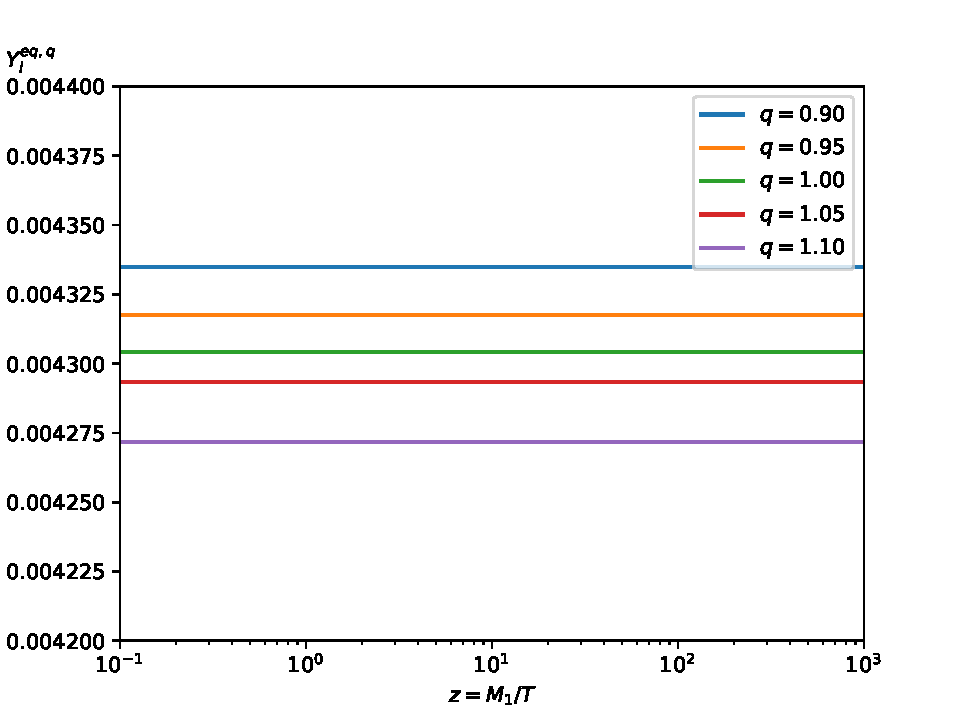
\includegraphics[width=13cm]{fig-YEql-nonextensive.pdf}
	\caption{تحول فراوانی تعادلی {\footnotesize${l_L}$} به ازای مقادیری از {\footnotesize$q$} با {\footnotesize$M_1 = 10^{11}\ \rm GeV$} \label{fig:YEql-nonextensive}}
\end{figure}
\begin{figure}[!h]
	\centering
	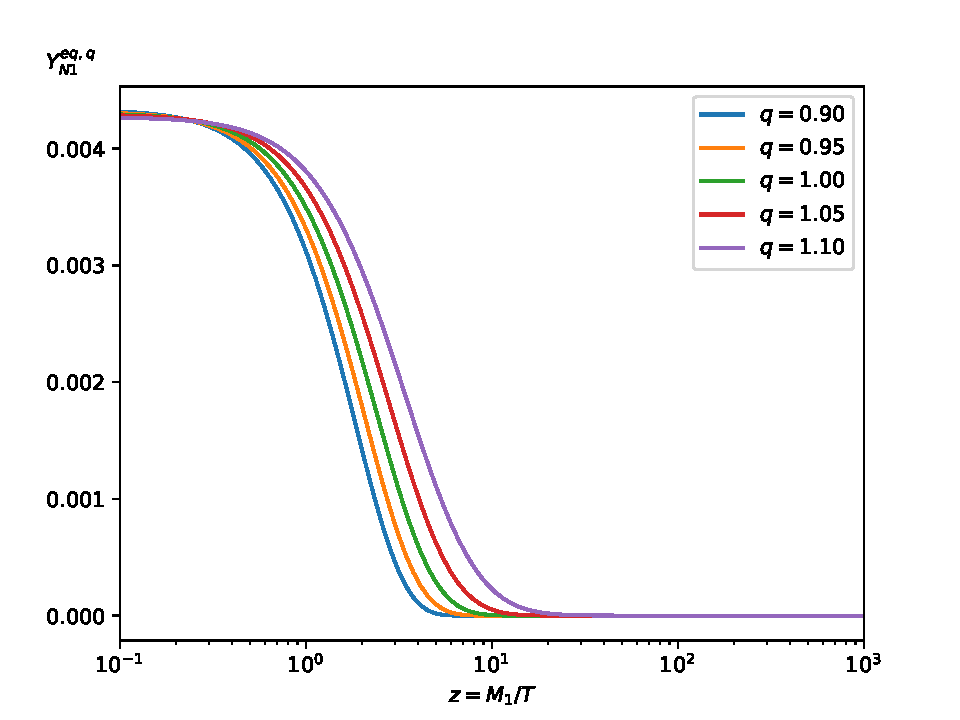
\includegraphics[width=13cm]{fig-YEqN1-nonextensive.pdf}
	\caption{تحول فراوانی تعادلی {\footnotesize$N_1$} به ازای مقادیری از {\footnotesize$q$} با {\footnotesize$M_1 = 10^{11}\ \rm GeV$} \label{fig:YEqN1-nonextensive}}
\end{figure}

\subsection{پارامتر واپاشی}
\label{sec:D1}
پارامتر واپاشی که در معادلات بولتزمان ظاهر شده، طبق معادله‌ی (\ref{eq:decay-parameter}) بصورت
{\footnotesize\begin{align}
	D^q_1 \equiv  \frac{2 \langle \Gamma_{1} \rangle}{H^q z},
	\label{eq:def-D1}
\end{align}}
تعریف می‌شود. می‌توان ابتدا میانگین گرمایی نرخ واپاشی را با توجه به (\ref{eq:average-decay-rate}) نوشت
{\footnotesize\begin{align}
	\langle \Gamma_{1} \rangle = \langle \overline{\Gamma}_1 \rangle =  \langle\frac{M_1}{E}\rangle \frac{M_1}{16 \pi} (yy^{\dagger})_{11}.
	\label{eq:averaged-decay-rate-nonextensive}
\end{align}}
حال می‌توان با جایگذاری نرخ انبساط هابل از معادله‌ی (\ref{eq:Hubble-nonextensive}) و نرخ واپاشی میانگین‌گیری شده از معادله‌ی (\ref{eq:averaged-decay-rate-nonextensive}) در تعریف پارامتر واپاشی (\ref{eq:def-D1}) بصورت
\par
\vspace{-0.5cm}
{\footnotesize\begin{align}
	D^q_1= \frac{2}{H^q z} \frac{\int_{0}^{\infty} \frac{dp\ p^2}{E} \left[ \frac{1}{e_q^{-(\frac{E_{N_1} z}{M_1})}}\right]^{-1}}{\int_{0}^{\infty} dp\ p^2 \left[ \frac{1}{e_q^{-(\frac{E_{N_1} z}{M_1})}}\right]^{-1}} \frac{M_1^2}{16 \pi} (yy^{\dagger})_{11},
	\label{eq:D1}
\end{align}}
بدست آورد.
با توجه به معادله‌ی (\ref{eq:D1}) پارامتر واپاشی را به ازای چند مقداری از {\footnotesize$q$} در شکل \ref{fig:D1-nonextensive} ترسیم کرده‌ایم. همانطور که مشاهده می‌شود، در حالت {\footnotesize$q>1$} افزایش پارامتر واپاشی نسبت به حالت {\footnotesize$q<1$} دیر‌تر رخ می‌دهد. این باعث تولید عدم تقارن در {\footnotesize$z$} های دیرتر از استاندارد برای حالت {\footnotesize$q>1$} می‌شود؛ برای حالت {\footnotesize$q<1$} نیز برعکس. اما بدلیل اینکه در دماهای بسیار بالا کار می‌کنیم، این نمی‌تواند روی عدم تقارن در نزدیکی گذار فاز التروضعیف تاثیر بگذارد.
\begin{figure}[!h]
	\centering
	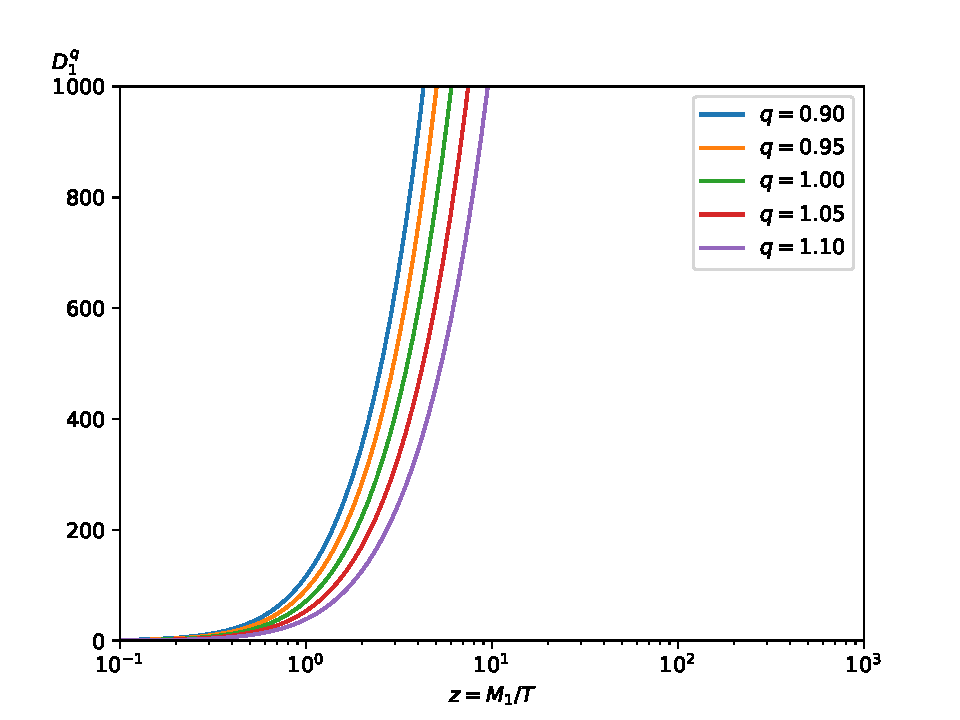
\includegraphics[width=13cm]{fig-D1-nonextensive.pdf}
	\caption{تحول پارامتر واپاشی به ازای مقادیری از {\footnotesize$q$} با {\footnotesize$M_1 = 10^{11}\ \rm GeV$} \label{fig:D1-nonextensive}}
\end{figure}

\subsection{پارامتر شستشو}
\label{sec:W1}
در معادلات بولتزمان پارامتر شستشو طبق معادله‌ی (\ref{eq:washout-parameter}) بصورت
{\footnotesize\begin{align}
	W^q_1 \equiv \frac{1}{2} \frac{Y_{N_1}^{{\rm eq},q}}{Y_{{l_L}}^{{\rm eq},q}} D^q_1,
	\label{eq:W1}
\end{align}}
تعریف می‌شود؛ که در آن {\footnotesize$Y^{{\rm eq},q}_{N_1}$} و {\footnotesize$Y^{{\rm eq},q}_{l_L}$} در بخش \ref{sec:YEq} و {\footnotesize$D_1^q$} در بخش \ref{sec:D1} توصیف شدند.
بنابراین می‌توان پارامتر شستشو را برای چند مقدار {\footnotesize$q$} ترسیم کرد. همانطور که در شکل \ref{fig:W1-nonextensive} نشان داده شده است، برای حالت {\footnotesize$q>1$} بر خلاف حالت {\footnotesize$q<1$}، مقدار بیشینه‌ی پارامتر شستشو در مقادیر بزرگ‌تر {\footnotesize$z$} اتفاق می‌افتد. این اثر مهم بر تولید عدم تقارن است، چراکه تجربه‌ی بیشینه‌ی شستشو در {\footnotesize$z$} های کوچک، زمانی که نوترینوهای راست دست هنوز به اندازه‌ی کافی ساخته نشده‌اند و هنوز \lr{\footnotesize CP} به مقدار ناچیزی نقض شده است، بدون اهمیت می‌شود. در این راستا، می توان پیش‌بینی کرد برای حالت {\footnotesize$q<1$} نقض \lr{\footnotesize CP} بیشتر اتفاق خواهد افتاد. از سوی دیگر پارامتر شستشو برای حالت {\footnotesize$q>1$} رشد می‌کند. بنابراین این نیز باعث کاهش عدم تقارن تولید شده خواهد شد.
\begin{figure}[!h]
	\centering
	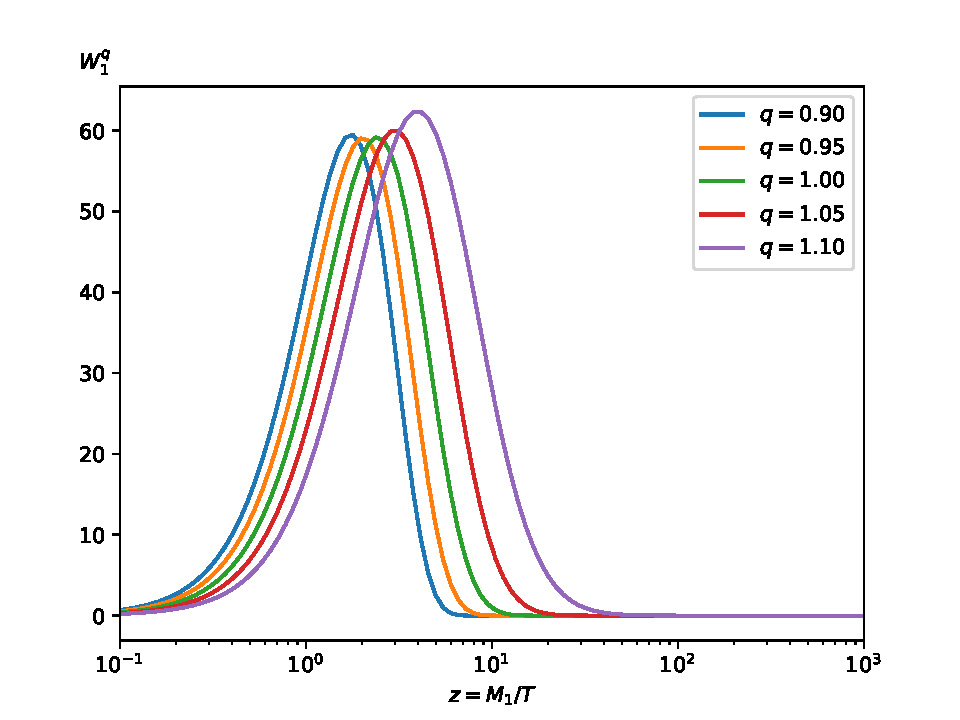
\includegraphics[width=13cm]{fig-W1-nonextensive.pdf}
	\caption{تحول پارامتر شستشو به ازای مقادیری از {\footnotesize$q$} با {\footnotesize$M_1 = 10^{11}\ \rm GeV$} \label{fig:W1-nonextensive}}
\end{figure}

\subsection{رابطه‌ی بین عدم تقارن \lr{\footnotesize B-L} و عدم تقارن باریون}
در نهایت، {\footnotesize$Y^q_{B-L}$} تولید شده توسط فرآیندهای اسفلرانی الکتروضعیف در نزدیکی گذار فاز الکتروضعیف می‌تواند به {\footnotesize$Y^q_B$} تبدیل شود. در واقع با در نظر داشتن شرط خنثی بودن ابربار، فرآیندهای اسفلرانی و تمام فرآیندهای چرخش چپ دستی و راست دستی می‌توان هماهنند معادله‌ی (\ref{eq:muBLtomuB}) نوشت
\par
\vspace{-0.5cm}
{\footnotesize\begin{align}
	\mu_B = \frac{28}{79} \mu_{B-L}.
	\label{eq:chemical-condition-nonextensive}
\end{align}}
توجه شود، پتانسیل شیمیایی با تعمیم مکانیک آماری تغییر نمی‌کند، چراکه پتاسیل شیمیایی یک مفهوم کلاسیکی در سطح ترمودینامیک است که به مکانیک آماری وابسطه نمی‌باشد.

حال می‌توان رابطه‌ی پتانسیل شیمیایی با عدم تقارن تولید شده را جستجو کرد. بدین مقصود، توجه شود که در جهان اولیه‌ای که با مکانیک آماری استاندارد توصیف می‌شود رابطه‌ی {\footnotesize$\frac{\mu}{T} \ll \frac{p}{T}$} برقرار است. از آنجایی که این نامعادله برای {\footnotesize$q=1$} برقرار است، با بسط حول این نقطه نیز برای مقادیر حول {\footnotesize$1$} نیز برقرار خواهد بود. با در نظر گرفتن مرتبه‌ی اول بسط معادله‌ی (\ref{eq:dist-nonextensive}) حول مقادیر {\footnotesize$|q-1|\ll1$} بدست می‌آید
\par
\vspace{-0.5cm}
{\footnotesize\begin{align}
	f^{q} = \frac{1}{e^{\beta \left(\epsilon-\mu\right)}+ \xi} + \frac{q-1}{2} \frac{\left[\beta \left(\epsilon-\mu\right)\right]^2 e^{\beta \left(\epsilon-\mu\right)}}{\left[e^{\beta \left(\epsilon-\mu\right)}+\xi\right]^2}.
	\label{eq:dist-app-nonextensive}
\end{align}}
بنابراین، توزیع ذرات و پادذرات از معادله‌ی (\ref{eq:dist-app-nonextensive}) بصورت تقریبی قابل بیان بصورت
{\footnotesize\begin{align}
	f^q = A + B \mu + O(\mu^2),\\
	\overline{f}^q = A - B \mu + O(\mu^2),
\end{align}}
است که در آن ثوابت {\footnotesize$A$} و {\footnotesize$B$} مستقل از {\footnotesize$\mu$} هستند. از آنجایی که مراتب صفر هر دو عبارت فوق برابرند، در {\footnotesize$n^q_i - \overline{n}_i^q$} سهمی نمی‌دهند. با احتساب سهم مراتب اول و بازتعریف ثابت جدید {\footnotesize$C$} تابعی از {\footnotesize$B$} می‌توان نوشت
\par
\vspace{-0.5cm}
{\footnotesize\begin{align}
	n^q_i - \overline{n}_i^q = C \mu.
\end{align}} 
بنابراین،‌ با تقسیم عبارت بدست آمده بر {\footnotesize$s^q$} می‌توان بین پتانسیل شیمیایی و عدم تقارن عبارت
{\footnotesize\begin{align}
	Y^q = \frac{C}{s^q} \mu.
\end{align}}
را بدست آورد. در آخر، می‌توان با ضرب دو سمت معادله‌ی (\ref{eq:chemical-condition-nonextensive}) در {\footnotesize$\frac{C}{s^q}$} می‌توان بدست آورد
{\footnotesize\begin{align}
	Y_{B}^q = \frac{28}{79} Y^q_{B-L}.
	\label{eq:relation-between-B-L-and-baryon-asymmetry-nonextensive}
\end{align}}

\section{نتایج عددی}
\label{sec:results-nonextensive}
در این بخش، قبل از پرداختن به حل عددی با استفاده از پارامتریزه کردن کازاس-ایبارا طبق معادله‌ی (\ref{eq:Casas-Ibarra-3}) استفاده می‌کنیم. با درنظر گرفتن ترتیب جرمی عادی، برای زوایای اختلاط و تفاضل جرم نوترینوهای سبک از داده‌های \lr{\footnotesize NuFIT 5.2} استفاده می‌کنیم \cite{Esteban:2020cvm} که در شکل (\ref{fig:NuFIT}) نیز به آن مقادیر اشاره شده است.
بطور خلاصه، ده پارامتر آزاد داریم که در جدول \ref{tab:parameters-nonextensive} بهمراه مقادیر در نظر گرفته شده‌شان بیان شده است.
\begin{table}[!h]
	\centering
	\caption{پارامتر‌های ثابت مدل}
	\begin{latin}
		\footnotesize
		\begin{tabular}{c c c c c c c c c c}
			\hline
			$m/{\rm GeV}$ & $M_1/{\rm GeV}$ & $M_2/{\rm GeV}$	& $M_3/{\rm GeV}$ & $x_1/\degree$ & $y_1/\degree$ & $x_2/\degree$ & $y_2/\degree$ & $x_3/\degree$ &   $y_3/\degree$ \\
			\hline
			$10^{-11}$	& $10^{11}$ & $10^{11.6}$& $10^{12}$ & $12$ & $51.4$ & $33$ & $11.4$ & $180$ & $11$\\
			\hline
		\end{tabular}
	\end{latin}
	\label{tab:parameters-nonextensive}
\end{table}

حال، می‌خواهیم بصورت عددی معادلات تحول بدست آمده را از نقطه‌ی شروع {\footnotesize$z_0=10^{-1}$} تا گذار فاز الکتروضعیف بطور همزمان با شرایط اولیه تهی از عدم تقارن حل کنیم. با حل معادلات، {\footnotesize$Y_{B-L}^q$} بدست آمده را در شکل \ref{fig:YBL-nonextensive} بنمایش گذاشته‌ایم. شرایط اولیه برای چند مقدار {\footnotesize$q$} در شکل‌ها مشخص شده‌اند. 

با انتخاب این فضای پارامتری برای مقادیر {\footnotesize$q<1.2$} در رژیم شستشوی قوی قرار خواهیم گرفت که با {\footnotesize$\Gamma_1 > H^q(T = M_1)$} تببین می‌شود. در این رژیم نتیجه‌ی نهایی مستقل از شرط {\footnotesize$Y^q_{N_1}(z_0)$} خواهد بود \cite{Buchmuller:2004nz}.
بنابراین {\footnotesize$Y_{N_1}^q(z_0)=0$} را در نظر می‌گیریم. از شکل \ref{fig:YBL-nonextensive} مشخص است که {\footnotesize$Y^q_{B-L}$} تولید شده برای {\footnotesize$q<1$} بیشتر و برای {\footnotesize$q>1$} کمتر از حالت استاندارد است. این نتیجه با بحث صورت گرفته در بخش \ref{sec:W1} همخوانی دارد. 
بنابراین با در نظر گرفتن مقادیر {\footnotesize$q<1$} می‌توان جرم نوترینوی راست دست مورد نیاز را برای تولید عدم تقارن انتظاری، کاهش داد. درنهایت، می‌توان در نزدیکی گذار فاز الکتروضعیف، {\footnotesize$Y^q_{B-L}$} تولید شده را توسط (\ref{eq:relation-between-B-L-and-baryon-asymmetry-nonextensive}) به عدم تقارن باریونی تبدیل کرد.
در شکل \ref{fig:YB-nonextensive} ما فضای پارامتری {\footnotesize$M_1$} و {\footnotesize$q$} مجاز را با در نظر گرفتن {\footnotesize$M_2=M_1 \times 10^{0.6}$} و {\footnotesize$M_3=M_1 \times 10^{1}$} که عدم تقارن باریونی مطلوب از طریق مکانیک آماری استاندارد و نافزونور در زمان الکتروضعیف بسازند را جستجو می‌کنیم.
\begin{figure}[!h]
\centering
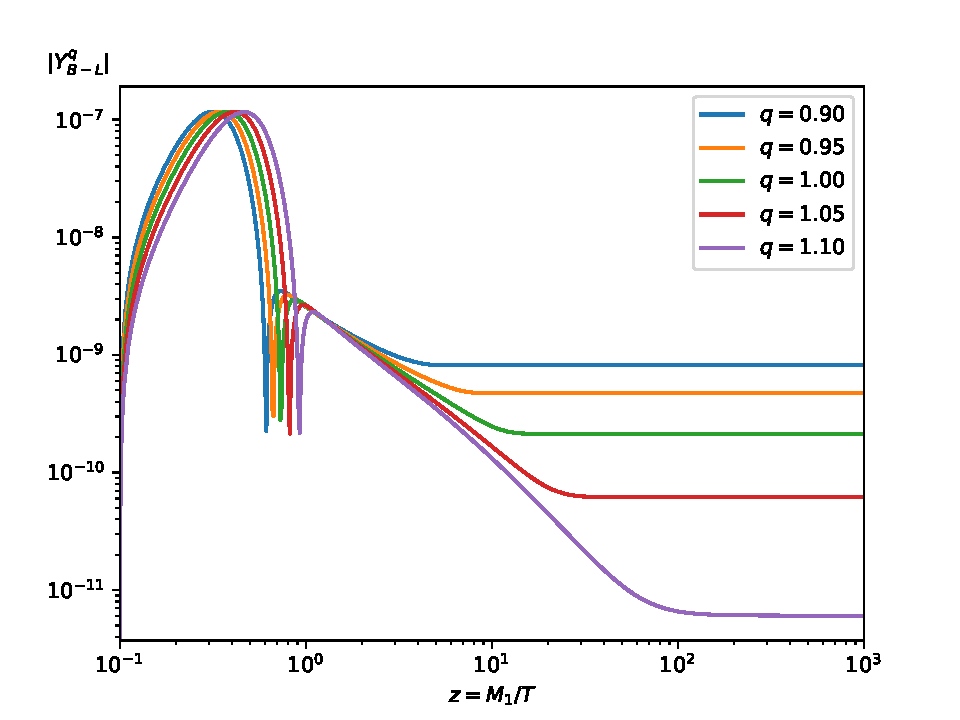
\includegraphics[width=13cm]{fig-BL-nonextensive.pdf}
	\caption{تحول {\footnotesize$|Y^q_{B-L}|$} به ازای مقادیری از {\footnotesize$q$} \label{fig:YBL-nonextensive}}
\end{figure}
\begin{figure}[!h]
	\centering
	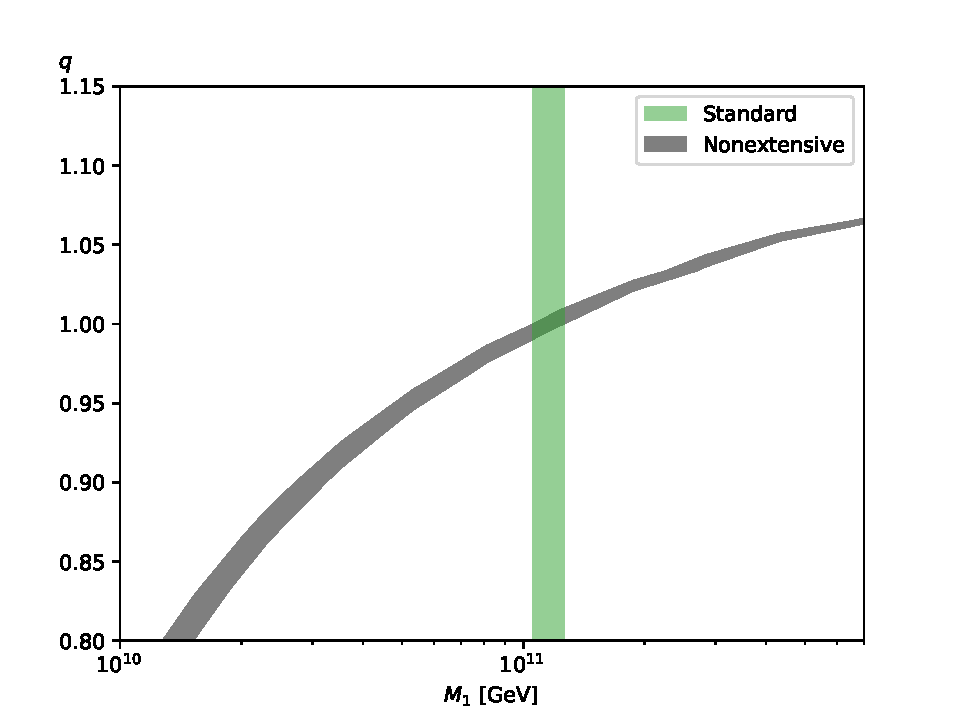
\includegraphics[width=13cm]{fig-B-nonextensive.pdf}
	\caption{ناحیه‌ی مجاز برای فضای پارامتری {\footnotesize$q$} و {\footnotesize$M_1$} برای تولید عدم تقارن {\footnotesize$Y^{\rm obs}_{B}$} با 5\% انحراف \label{fig:YB-nonextensive}}
\end{figure}

\chapter{لپتون‌زایی گرمایی در کیهان ناهمسانگرد}
\label{chap:anisotropic}
هیچ شواهدی بر اینکه عالم قبل از هسته‌زایی مه‌بانگ همگن و همسانگرد باشد، وجود ندارد. کیهان‌شناسی بیانکی نوع اول ساده‌ترین کیهان‌شناسی همگن ولی ناهمسانگرد است. در این فصل،‌ما به بررسی لپتون‌زایی گرمایی به عنوان یک سناریوی باریون‌زایی، در کیهان‌شناسی بیانکی نوع اول می‌پردازیم. نتایج ما نشان می‌دهد که برای مقادیر خاصی از ناهمسانگردی، لپتون‌زایی گرمایی تعمیم‌یافته عدم تقارن بیشتری نسبت به مورد استاندارد تولید می‌کند. در این راستا، ناهمسانگردی می‌تواند به دست‌یابی به لپتون‌زایی مقیاس کم موثر واقع شود.
\section{مقدمه}
در این فصل، ما بر نوعی از کیهان‌شناسی غیر استاندارد که با نادیده گرفتن اصل کیهان‌شناختی همسانگردی بدست می‌آید، تمرکز می‌کنیم. از آنجایی که هیچ نشانه‌ای از همسانگردی قبل از هسته‌زایی مه‌بانگ وجود ندارد، این فرض معقول بنظر می‌رسد. علاوه بر آن، افزایش دقت مشاهدات اخیر، تنش‌هایی در مدل استاندارد کیهان‌شناسی بوجود آورده‌اند \cite{Verde:2019ivm,DiValentino:2020zio,DiValentino:2021izs}. تلاش‌های کثیری در راستای کاهش این تنش‌ها انجام شده است \cite{Abdalla:2022yfr,Perivolaropoulos:2021jda}. این تنش‌ها باعث ایجاد حساسیت نسبت به درستی اصول کیهان‌شناختی همگنی و همسانگردی شده است \cite{Colgain:2022tql,Colgain:2022rxy,Krishnan:2021dyb,Krishnan:2021jmh,PhysRevD.100.023532}. برای مرور این موضوع می‌توان به مرجع \cite{Aluri:2022hzs} مراجعه کرد. به این دلیل اخیرا شاهد مدل‌های ناهمسانگرد بوده‌ایم. معروف‌ترین رده‌ی این مدل‌ها به کیهان‌شناسی بیانکی است \cite{Ellis:1968vb}. در میان آنها، بیانکی نوع اول، ساده‌ترین آنها است که در این فصل به آن متمرکز می‌شویم. برای اطلاعات بیشتر در مورد کیهان‌شناسی بیانکی نوع اول می‌توان به مراجع . رجوع کرد \cite{delliou_anisotropic_2020,Russell:2013oda,jacobs1969bianchi}. اینجا، ما در جستجوی اثر ناهمسانگردی عالم بر لپتون‌زایی گرمایی با سه نوترینوی راست دست هستیم. در این راستا، ما نشان می‌دهیم که نرخ انبساط هابل تغییر می‌کند که باعث جهش زمان افزایش پارامتر واپاشی، کاهش شستشو و کاهش مقدار نوترینوی راست دست تولید شده می‌شود. همانطور که در ادامه اشاره خواهیم کرد، اثر جابجایی پارامتر واپاشی قابل چشم‌پوشی است. همینطور، واضح است که کاهش شستشو باعت افزایش عدم تقارن می‌شود. در مقابل آن، کاهش تولید نوترینوی راست دست منجر به نقض کمتر تقارن \lr{\footnotesize CP} می‌شود. به عنوان نتیجه این رقابت، مقادیر خاصی از ناهمسانگردی می‌تواند عدم تقارن باریونی بیشتری نسبت به مورد استاندارد تولید کند.

پیکربندی این فصل به شرح زیر تنظیم شده است. در بخش \ref{sec:anisotropic}، مقدمه‌ای بر کیهان‌شناسی ناهمسانگرد بیانکی نوع اول مطرح می‌کنیم. در بخش \ref{sec:modifeid-leptogenesis-anisotropic}، با مروری بر لپتون‌زایی گرمایی بر اثر ناهمسانگردی بر آن می‌پردازیم. در بخش \ref{sec:results-anisotropic}، با معرفی فضای پارامتر به استخراج نتایج عددی از معادلات بدست آمده می‌پردازیم.

\section{کیهان‌شناسی ناهمسانگرد بیانکی نوع اول}
\label{sec:anisotropic}
‌کیهان‌شناسی استاندارد بر پایه‌ی متریک \lr{\footnotesize FLRW} استوار است. در متریک \lr{\footnotesize FLRW} فرض بر این است که قسمت فضایی تخت باشد و اصول کیهان‌شناختی: همگنی و همسانگردی در بزرگ مقیاس برقرار باشند. در حالی که کیهان‌شناسی بیانکی یکی از جایگزین‌های استاندارد است که همسانگردی را کنار می‌گذارد. نمونه‌ی ساده‌ای از عالم بیانکی توسط متریک بیانکی نوع اول بیان می‌شود \cite{Ellis:1968vb,delliou_anisotropic_2020,Russell:2013oda,jacobs1969bianchi}
\par
\vspace{-0.5cm}
{\footnotesize\begin{align}
	ds^2 = -dt^2 + a_1^2(t) dx^2 + a_2^2(t) dy^2 + a_3^2(t) dz^2,
	\label{eq:BI-metric-anisotropic}
\end{align}}
که در آن {\footnotesize$a_i$} عامل مقیاس جهتی و بدین ترتیب نرخ انبساط هابلی جهتی بصورت {\footnotesize$H_i=\dot{a_i}/a_i$} قابل محاسبه است.

از آنجایی که به مطالعه‌ی جهان اولیه علاقه‌مند هستیم، معادله فریدمان تعمیم‌یافته در دوره‌ی تابش غالب با چگالی انرژی {\footnotesize$\epsilon_r \propto a^{-4}$} بصورت
\par
\vspace{-0.5cm}
{\footnotesize\begin{align}
	H^2 = \frac{8 \pi G}{3} \epsilon_r + \frac{1}{3} \sigma^2,
	\label{eq:Friedmann-Eq.-anisotropic}
\end{align}}
که در آن عامل مقیاس و نرخ هابل موثر بصورت
{\footnotesize\begin{align}
	a \equiv \left(a_1 a_2 a_3\right)^{1/3}, \quad H \equiv\dot{a}/a = \frac{1}{3} \left(H_1+H_2+H_3\right).
	\label{eq:Hubble-definition-anisotropic}
\end{align}}
تعریف شده است. در معادله‌ی فریدمان، ناهمسانگردی عالم با مجذور نرده‌ای برشی  بیان می‌شود؛ که بصورت
{\footnotesize\begin{align}
	\sigma^2 \equiv \frac{1}{6} \left[\left(H_1-H_2\right)^2+\left(H_2-H_3\right)^2+\left(H_3-H_1\right)^2\right].
\end{align}}
تعریف می‌شود. با توجه به رابطه‌ی کاربردی {\footnotesize$\dot{H}_i - \dot{H}_j = -3 H \left(H_i - H_j\right)$} که معادل {\footnotesize$H_i - H_j \propto a^{-3}$} است، می‌توان وابستگی مجذور نرده‌ای برشی را بر عامل مقیاس موثر را بصورت {\footnotesize$\sigma^2 \propto a^{-6}$} بدست آورد. بنابراین، مجذور نرده‌ای برشی سریع‌تر از چگالی انرژی بی‌اثر می‌شود.
									
دمای {\footnotesize$T_e$} را بصورتی که در آن {\footnotesize$8 \pi G \epsilon_r=\sigma^2$} برقرار باشد تعریف می‌کنیم. زمانی که {\footnotesize$T\gg T_e$} باشد، عالم برشی غالب است: لذا روابط {\footnotesize$H \propto a^{-3}$} و {\footnotesize$a \propto t^{1/3}$} یا به عبارتی {\footnotesize$H = 1/3t$} برقرار است؛ زمانی که {\footnotesize$T \ll T_e$} باشد، عالم تابش غالب است: لذا روابط {\footnotesize$H \propto a^{-2}$} و {\footnotesize$a \propto t^{1/2}$} یا به عبارتی {\footnotesize$H = 1/2t$} برقرار است.
بنابراین، می‌توان از دمای {\footnotesize$T_e$} بعنوان میزان ناهمسانگردی تعبیر کرد؛ مقادیر کوچک {\footnotesize$T_e$}، میزان ناهمسانگردی بیشتر و برعکس.
می‌توان مجذور نرده‌ای برشی را برحسب چگالی انرژی تابش بدست آورده و سپس نرخ انبساط هابل را بصورت \cite{PhysRevD.42.3310}
\par
\vspace{-0.5cm}
{\footnotesize\begin{align}
	H=\frac{1.66}{M_{Pl}} (g_{\star})^{1/2} T^2 \sqrt{1+\frac{g_{\star}}{g^e_{\star}}\frac{T^2}{T^2_e}},
	\label{eq:Hubble-anisotropic}
\end{align}}
بیان کرد که در آن {\footnotesize$M_{Pl} = 1.22 \times 10^{19}$} جرم پلانک،{$g_{\star}$} و {\footnotesize$g_{\star}^e$} بترتیب درجات آزادی موثر چگالی انرژی در دماهای {\footnotesize$T$} و {\footnotesize$T_e$} هستند.
توجه شود که در حد {\footnotesize$T_e \to \infty$} معادله‌ی (\ref{eq:Hubble-anisotropic}) به نرخ هابل متداول برمی‌گردد. از آنجایی که هیچ نشانه‌ای از ناهمسانگردی در هسته‌زایی مهباگ دیده نمی‌شود، می‌خواهیم ناهمسانگری اثری نداشته باشد؛ لذا قید {\footnotesize$T_e\gg 2.5\ \rm MeV$} را خواهیم داشت \cite{PhysRevD.42.3310}. لذا طبق مرجع \cite{Husdal:2016haj} ،{$g_{\star}$} و {\footnotesize$g_{\star}^e$} را تقریبا برابر {\footnotesize$106.75$} می‌توان در نظر گرفت.

\section{لپتون‌زایی تعمیم یافته}
\label{sec:modifeid-leptogenesis-anisotropic}
تمام جزئیات لپتون‌زایی گرمایی استاندارد که در فصل \ref{chap:leptogenesis} بررسی شد را در نظر می‌گیریم.
حال، می‌خواهیم تحول نوترینوی راست دست با تابع توزیع {\footnotesize$f_{N_1}=f_{N_1}(x^{\alpha},p^{\alpha})$} را بیان کنیم. شکل کلاسیکی معادله تحول توسط معادله‌ی بولتزمان بیان می‌شود
\par
\vspace{-0.5cm}
{\footnotesize\begin{align}
	\boldsymbol{L}[f_{N_1}]=\boldsymbol{C}[f_{N_1}]
	\label{eq:Boltzmann-anisotropic},
\end{align}}
که در آن {\footnotesize$\boldsymbol{L}$} اپراتور لیوویل است که تغییرات ذره‌ها با پارامترهای دینامیکی را توصیف می‌کند و {\footnotesize$\boldsymbol{C}$} اپراتور برخورد است که چشمه‌ی تحولات فرآیندهای میکروسکوپی است.

با اختلال در متریک، انتظار داریم اپراتور برخورد بدون تغییر باقی بماند و همان شکل استاندارد را همانند معادله‌ی (\ref{eq:collision}) دارا می‌باشد. اگرچه اپراتور لیوویل تحت تاثیر قرار می‌گیرد. همانطور که در معادله‌ی (\ref{eq:liouville}) بیان شده، شکل نسبیتی اپراتور لیوویل بصورت
\par
\vspace{-0.5cm}
{\footnotesize\begin{align}
		\boldsymbol{L}=p^{\alpha}\frac{\partial}{\partial x^{\alpha}}-\Gamma^{\alpha}_{\beta \gamma} p^{\beta} p^{\gamma} \frac{\partial}{\partial p^{\alpha}},
		\label{eq:Liouville-anisotropic}
\end{align}}
است که {\footnotesize$\Gamma^{\alpha}_{\beta \gamma}$} ها نمادهای کریستوفل متریک مربوطه هستند. برای متریک بیانکی نوع اول، نمادهای کریستوفل غیر صفر برابرند با
\par
\vspace{-0.5cm}
{\footnotesize\begin{align}
	\Gamma^{1}_{0 1}=\Gamma^{1}_{1 0}&=\frac{\dot{a_1}}{a_1}, \quad \Gamma^{2}_{0 2}=\Gamma^{2}_{2 0}=\frac{\dot{a_2}}{a_2}, \quad \Gamma^{3}_{0 3}=\Gamma^{3}_{3 0}=\frac{\dot{a_3}}{a_3}, \notag  \\
	&\Gamma^{0}_{1 1}=a_1\dot{a_1}, \quad \Gamma^{0}_{2 2}=a_2\dot{a_2}, \quad \Gamma^{0}_{3 3}=a_3\dot{a_3}.
	\label{eq:Christoffel-anisotropic}
\end{align}}
با جایگذاری نمادهای کریستوفل (\ref{eq:Christoffel-anisotropic}) در اپراتور لیوویل (\ref{eq:Liouville-anisotropic})، معادله بولتزمان (\ref{eq:Boltzmann-anisotropic}) بصورت
{\footnotesize\begin{align}
	\frac{\partial f_{N_1}}{\partial t} - 2 \frac{\dot{a_1}}{a_1} p^1 \frac{\partial f_{N_1}}{\partial p^1} - 2 \frac{\dot{a_2}}{a_2} p^2 \frac{\partial f_{N_1}}{\partial p^2} - 2 \frac{\dot{a_3}}{a_3} p^3 \frac{\partial f_{N_1}}{\partial p^3} = \frac{1}{p^0} \boldsymbol{C}[f_{N_1}].
	\label{eq:anisotropic-Boltzmann}
\end{align}}
بدست می‌آید. با توجه به تعریف نرخ هابل (\ref{eq:Hubble-anisotropic}) و تعریف چگالی تعداد نوترینوهای راست دست {\footnotesize$n_{N_1}=\frac{g_{N_1}}{(2\pi)^3}\int d^3p f$} که در آن {\footnotesize$g_{N_1}=2$} تعداد درجات آزادی متناظرش است، معادله‌ی (\ref{eq:anisotropic-Boltzmann}) بصورت زیر می‌شود؛
\par
\vspace{-0.5cm}
{\footnotesize\begin{align}
	\frac{dn_{N_1}}{dt}+3Hn_{N_1} = \frac{g_{N_1}}{(2\pi)^3} \int \boldsymbol{C}[f_{N_1}] \frac{d^3p}{p^0}.
\end{align}}
حال باتوجه به رابطه‌ی {\footnotesize$sa^3=\rm const.$} که {\footnotesize$s$} آنتروپی است و تعریف {\footnotesize$Y_{N_1} \equiv n_{N_1}/s$}، می‌توان رابطه‌ی اخیر را بصورت زیر ساده کرد؛
{\footnotesize\begin{align}
	\frac{dY_{N_1}}{dt} = \frac{g_{N_1}}{s (2\pi)^3} \int \boldsymbol{C}[f] \frac{d^3p}{p^0}.
\end{align}}
در نهایت، سمت راست معادله‌ی فوق را می‌توان از فصل \ref{chap:leptogenesis} جایگذاری کرد؛
{\footnotesize\begin{align}
	\frac{dY_{N_1}}{dz} = \frac{dt}{dT} \frac{dT}{dz} \left[- 2 \langle \Gamma_1 \rangle \left( Y_{N_1} - Y_{N_1}^{{\rm eq}} \right)\right].
	\label{eq:anisotropic-Boltzmann-l}
\end{align}}
									
به همین منوال می‌توان معادله‌ی بولتزمان {\footnotesize$Y_{B-L}\equiv (\overline{n}_{l_L} - n_{l_L})/s$} را طبق اپراتور لیوویل متناظرش از فصل \ref{chap:leptogenesis} بصورت
\par
\vspace{-0.5cm}
{\footnotesize\begin{align}
	\frac{dY_{B-L}}{dz} = \frac{dt}{dT} \frac{dT}{dz} \left[- \epsilon_1 2 \langle \Gamma_1 \rangle \left( Y_{N_1} - Y_{N_1}^{{\rm eq}} \right) - \frac{Y_{N_1}^{{\rm eq}}}{Y_{{l_L}}^{{\rm eq}}} \langle \Gamma_{1} \rangle Y_{B-L}\right],
	\label{eq:anisotropic-Boltzmann-r}
\end{align}}
نوشت که در آن {\footnotesize$Y_{{l_L}}^{{\rm eq}}$} چگالی تعداد تعادلی لپتون‌ها هستند که در ادامه، در معادله‌ی (\ref{eq:YEq-anisotropic}) بیان خواهد شد.
									
حال برای بدست آوردن {\footnotesize$\frac{dt}{dT} \frac{dT}{dz}$} نیازمند رابطه‌ای میان {\footnotesize$z$} و {\footnotesize$T$} که توسط {\footnotesize$z=M_1/T$} واضح است و رابطه‌ای میان {\footnotesize$t$} و {\footnotesize$T$} است.
باتوجه به بخش \ref{sec:anisotropic}، از آنجایی که رابطه‌ی {\footnotesize$H = 1/pt$} با {\footnotesize$p=2$} برای تابش غالب و با {\footnotesize$p=3$} برای برشی غالب برقرار است؛ می‌توان رابطه‌ی {\footnotesize$t$} و {\footnotesize$T$}  را بصورت {\footnotesize$tT^p=\rm constant$} یافت. بنابراین می‌توان بدست آورد؛
\par
\vspace{-0.5cm}
{\footnotesize\begin{align}
	\frac{dt}{dT} \frac{dT}{dz} = \frac{1}{Hz}.
\end{align}}

می‌توان معادلات بولتزمان (\ref{eq:anisotropic-Boltzmann-l}) و (\ref{eq:anisotropic-Boltzmann-r}) را بصورت
{\footnotesize\begin{align}
	\frac{dY_{N_1}}{dz} &= -D_1 \left( Y_{N_1} - Y_{N_1}^{{\rm eq}} \right),\\
	\frac{dY_{B-L}}{dz} &= - \epsilon_1 D_1 \left( Y_{N_1} - Y_{N_1}^{{\rm eq}} \right) - W_1 Y_{B-L},
\end{align}}
ساده کرد؛ که در آن پارامتر واپاشی {\footnotesize$D_1$} و شستشو {$W_1$} بصورت
{\footnotesize\begin{align}
	D_1 \equiv  \frac{2 \langle \Gamma_{1} \rangle}{H z}, \quad
	W_1 \equiv \frac{1}{2} \frac{Y_{N_1}^{{\rm eq}}}{Y_{{l_L}}^{{\rm eq}}} D_1,
	\label{eq:D1W1-anisotropic}
\end{align}}
تعریف می‌شود. در معادلات فوق {\footnotesize$Y_{\chi}^{{\rm eq}}$} به چگالی تعداد تعادلی {\footnotesize$\chi$} اشاره دارد که بصورت
{\footnotesize\begin{align}
	Y_{N_1}^{{\rm eq}} = \frac{45}{4 \pi^4} \frac{g_{N_1}}{g_{\star}} z^2 K_2(z), \quad 
	Y_{{l_L}}^{{\rm eq}} \simeq \frac{45}{4 \pi^4} \frac{g_{{l_L}}}{g_{\star}} \frac{3}{2} \zeta(3),
	\label{eq:YEq-anisotropic}
\end{align}}
بیان می‌شود که در آن {\footnotesize$g_{N_1}=g_{{l_L}}=2$} تعداد درجات آزادی و {\footnotesize$\zeta(s)$} تابع زتا است.

با توجه به معادله‌ی (\ref{eq:D1W1-anisotropic}) پارامتر واپاشی را به ازای چند مقدار {\footnotesize$T_e$} در شکل \ref{fig:D1-anisotropic} ترسیم می‌کنیم. همانطور که قابل مشاهده است برای حالت {\footnotesize$T_e<M_1$} افزایش پارامتر واپاشی دیرتر از حالت {\footnotesize$T_e>M_1$} اتفاق می‌افتد که تاثیری بر تولید عدم تقارن در نهایت، نخواهد داشت چرا که تولید عدم تقارن در دماهای خیلی بالا رخ می‌دهد.

همانند پارامتر واپاشی، می‌توان طبق معادله‌ی (\ref{eq:D1W1-anisotropic}) پارامتر شستشو را به ازای چند مقدار {\footnotesize$T_e$} ترسیم کرد. همانطور که در شکل \ref{fig:W1-anisotropic} می‌توان دید، برای حالت {\footnotesize$T_e<M_1$} در کنار کاهش شدت شستشو، نقطه‌ی بیشینه‌ی آن نیز به دماهای پایین جابجا می‌شود. اما با کاهش شدت، جابجا شدن نقطه‌ی بیشینه چندان اهمیت ندارد.
\begin{figure}[!h]
	\centering
	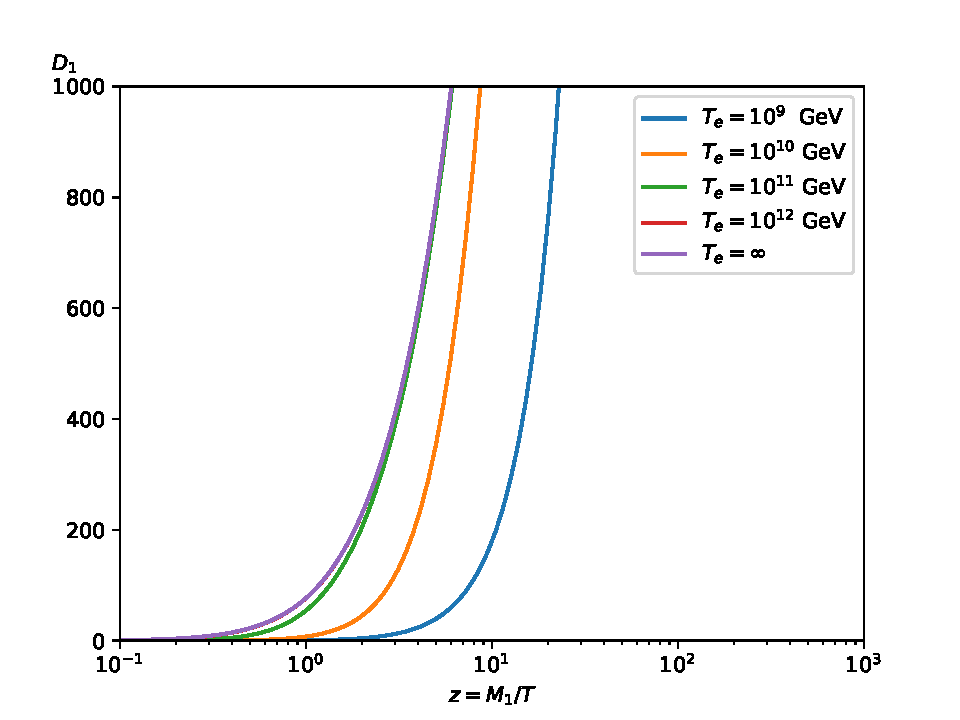
\includegraphics[width=13cm]{fig-D1-anisotropic.pdf}
	\caption{تحول پارامتر واپاشی به ازای مقادیری از {\footnotesize$T_e$} با {\footnotesize$M_1 = 10^{11}\ \rm GeV$} \label{fig:D1-anisotropic}}
\end{figure}
\begin{figure}[!h]
	\centering
	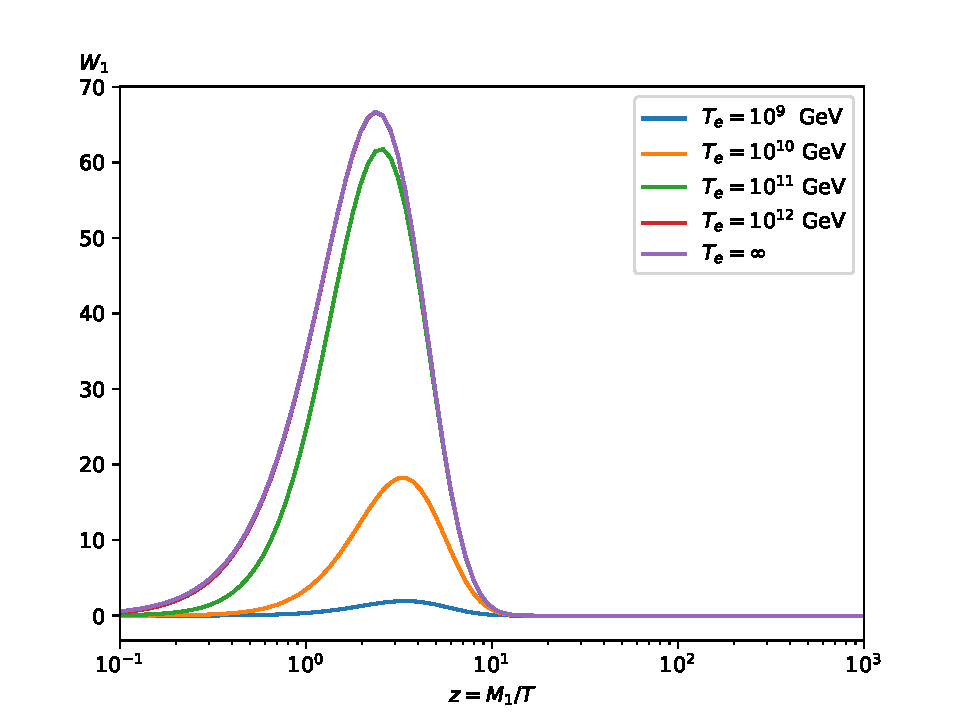
\includegraphics[width=13cm]{fig-W1-anisotropic.pdf}
	\caption{تحول پارامتر شستشو به ازای مقادیری از {\footnotesize$T_e$} با {\footnotesize$M_1 = 10^{11}\ \rm GeV$} \label{fig:W1-anisotropic}}
\end{figure}

{\footnotesize$Y_{B-L}$} تولید شده می‌تواند با توجه به فرآیندهای اسفلرانی الکتروضعیف به عدم تقارن باریونی تبدیل شود. با توجه به قیود مذکور در بخش \ref{sec:baryon-asymmetry} می‌توان همانند معادله‌ی (\ref{eq:YBLtoYB}) نوشت
{\footnotesize\begin{align}
	Y_{B} = \frac{28}{79} Y_{B-L}.
	\label{eq:YBLtoB-anisotropic}
\end{align}}

\section{نتایج عددی}
\label{sec:results-anisotropic}
در این بخش، قبل از پرداختن به حل عددی با استفاده از پارامتریزه کردن کازاس-ایبارا طبق معادله‌ی (\ref{eq:Casas-Ibarra-3}) استفاده می‌کنیم. بطور خلاصه، ده پارامتر آزاد داریم که در جدول \ref{tab:parameters-anisotropic} بهمراه مقادیر در نظر گرفته شده‌شان بیان شده است.
\begin{table}[!h]
	\centering
	\caption{پارامتر‌های ثابت مدل}
	\begin{latin}
		\footnotesize
		\begin{tabular}{c c c c c c c c c c}
			\hline
			$m/{\rm GeV}$ & $M_1/{\rm GeV}$ & $M_2/{\rm GeV}$	& $M_3/{\rm GeV}$ & $x_1/\degree$ & $y_1/\degree$ & $x_2/\degree$ & $y_2/\degree$ & $x_3/\degree$ &   $y_3/\degree$ \\
			\hline
			$10^{-11}$	& $10^{11}$ & $10^{11.6}$& $10^{12}$ & $12$ & $51.4$ & $33$ & $11.4$ & $180$ & $11$\\
			\hline
		\end{tabular}
	\end{latin}
	\label{tab:parameters-anisotropic}
\end{table}

حال معادلات تحول را بطور همزمان بصورت عددی از نقطه‌ی آغاز {\footnotesize$z_0=10^{-1}$} تا گذار فاز الکتروضعیف بدون عدم تقارن اولیه حل می‌کنیم. پاسخ {\footnotesize$Y_{N_1}$} و {\footnotesize$Y_{B-L}^q$} به ازای چند مقادیری از {\footnotesize$T_e$} بترتیب در شکل‌های \ref{fig:YBL-anisotropic} و \ref{fig:YN1-anisotropic} نشان داده شده‌اند.
با بررسی فضای پارامتر اتخاذ شده، برای مقادیر {\footnotesize$T_e>10^9\ {\rm GeV}$} در رژیم شستشوی قوی قرار می‌گیریم که با {\footnotesize$\Gamma_1 > H(T = M_1)$} تبیین می‌شود. در این رژیم نتیجه‌ی نهایی از مقدار {\footnotesize$Y^q_{N_1}(z_0)$} مستقل است \cite{Buchmuller:2004nz}. بنابراین در ابتدا فرض می‌کنیم {\footnotesize$Y_{N_1}^q(z_0)=0$}.

بعنوان اولین نتیجه، همانطور که در شکل \ref{fig:YN1-anisotropic} قابل ملاحظه است؛ برای حالت {\footnotesize$T_e<M_1$} تولید {\footnotesize$Y_{N_1}$} دیرتر شروع می‌شود. بنابراین برای حالت {\footnotesize$T_e<M_1$} بیشینه‌ی مقدار تولید شده‌ی نوترینوی راست دست کاهش می‌یابد. لذا انتظار داریم در اثر کاهش واپاشی نوترینوی راست دست، نقض \lr{\footnotesize CP} و در نتیجه عدم تقارن تولید شده نیز کاهش یابد. این اثر کاهش عدم تقارن در تقابل با اثر افزایش عدم تقارن از طریق کاهش پارامتر واپاشی است که در شکل \ref{fig:W1-anisotropic} اشاره شد.
\begin{figure}[!h]
	\centering
	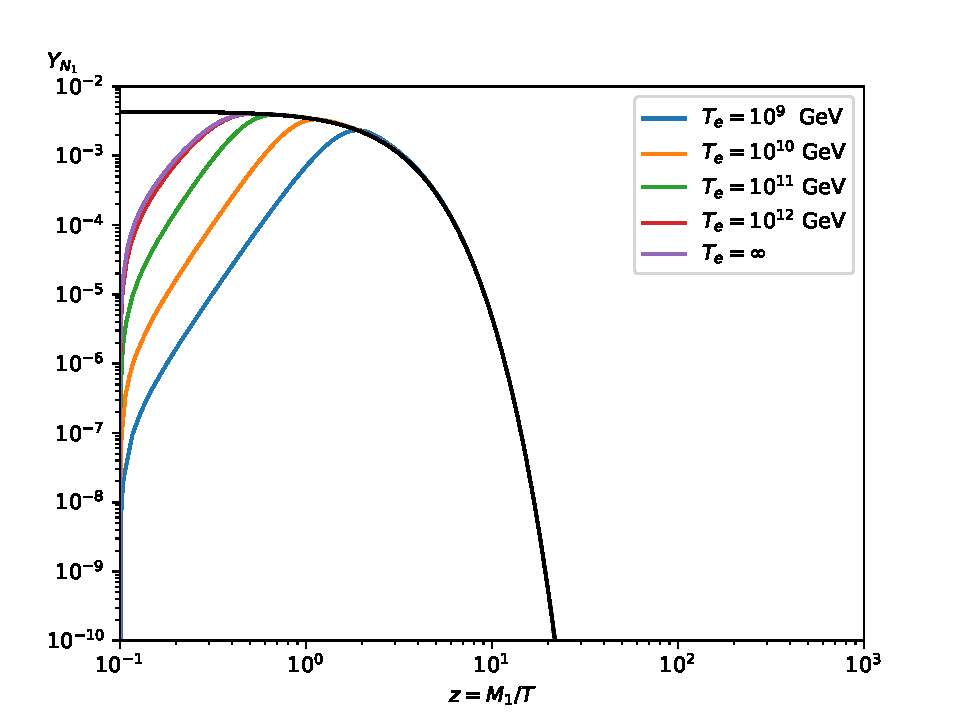
\includegraphics[width=13cm]{fig-N1-anisotropic.pdf}
	\caption{تحول {\footnotesize$Y_{N_1}$} به ازای مقادیری از {\footnotesize$T_e$} \label{fig:YN1-anisotropic}}
\end{figure}
توجه به این نکته مهم است که برای مقادیر {\footnotesize$T_e>10^9\ {\rm GeV}$} این اثر با توجه به اینکه در رژیم شستشوی قوی هستیم قابل صرف نظر بوده و می‌توان از آن صرف نظر کرد. اگرچه برای مقادیر {\footnotesize$T_e<10^9\ {\rm GeV}$} این اثر با در نظر گرفتن مقدار اولیه نوترینوی راست دست که از طریق غیر گرمایی تولید شده باشد، قابل خنثی شدن است \cite{Giudice:2003jh}.

در شکل \ref{fig:YBL-anisotropic}، {\footnotesize$|Y_{B-L}|$} به ازای مقادیری از {\footnotesize$T_e$} نمایش داده شده است. همانطور که می‌توان دید، شدت شستشو برای حالت {\footnotesize$T_e<M_1$} ضعیف‌تر است. بیشینه مقدار {\footnotesize$Y_{B-L}$} نیز بدلیلی که در پاراگراف اخیر ذکر شد کاهش پیدا کرده است. همینطور جابجا شدن مقدار بیشینه‌ی {\footnotesize$Y_{B-L}$} به دماهای کم برای حالت {\footnotesize$T_e<M_1$} با تاخیر در افزایش پارامتر واپاشی در ارتباط است که در شکل \ref{fig:D1-anisotropic} به آن اشاره شد.

برای درک بهتر افزایش عدم تقارن از طریق کاهش پارامتر واپاشی و کاهش عدم تقارن از طریق رفتار {\footnotesize$Y_{N_1}$}، {\footnotesize$Y_B$} را با توجه به رابطه‌ی (\ref{eq:YBLtoB-anisotropic}) از {\footnotesize$Y_{B-L}$} بدست آورده و در زمان گذار فاز الکتروضعیف بر حسب {\footnotesize$T_e$} برای مقادیر مختلف اولیه نوترینوی راست دست رسم می‌کنیم.
همانطور که در شکل \ref{fig:YB-anisotropic} قابل مشاهده است، تاثیری بر حالت‌های {\footnotesize$T_e>M_1$} شاهد نمی‌باشیم. در ثانی، همانطور که انتظار داشتیم برای مقادیر {\footnotesize$T>10^9\ {\rm GeV}$} نتیجه‌ی نهایی به مقدار اولیه فراوانی نوترینوی راست دست وابسته نمی‌باشد. همیچنین، عدم تقارن باریونی در این میزان ناهمسانگردی افزایش پیدا کرده است. سوما، برای مقادیر {\footnotesize$T_e<10^9\ {\rm GeV}$} همانطور که بحث شد، عدم تقارن باریونی بسته به اینکه مقدار اولیه‌ی فراوانی نوترینوی راست دست چقدر باشد می‌تواند زیاد یا کمتر باشد. در نتیجه لپتون‌زایی می‌تواند با مقیاس‌های پایین‌تر انرژی قابل بررسی قرار گیرد \cite{Chun:2017spz}.
\begin{figure}[b]
	\centering
	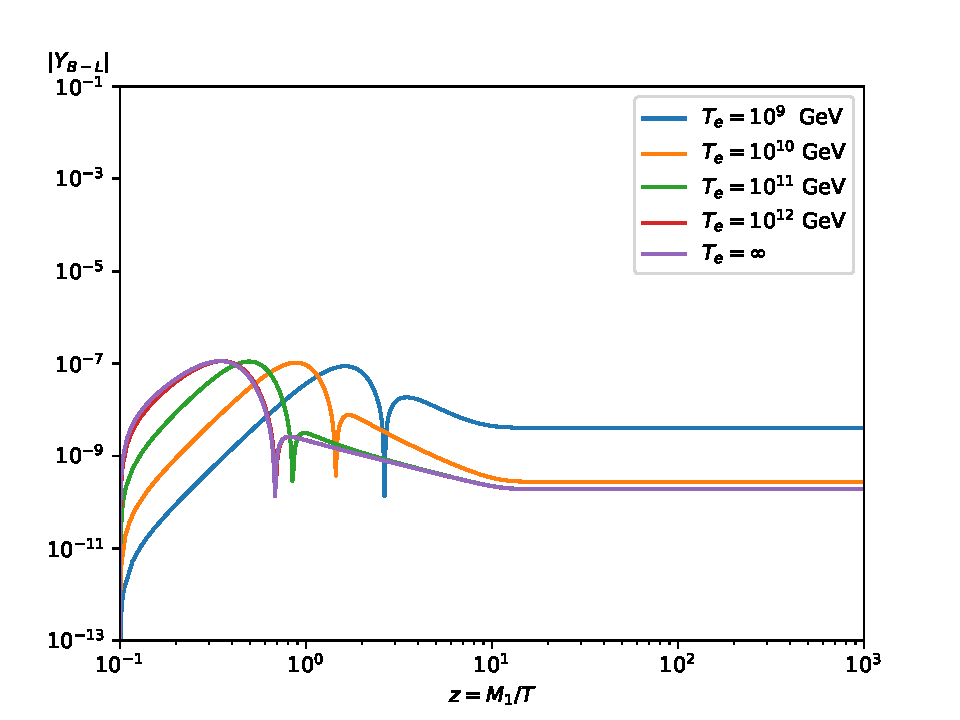
\includegraphics[width=13cm]{fig-BL-anisotropic.pdf}
	\caption{تحول {\footnotesize$|Y_{B-L}|$} به ازای مقادیری از {\footnotesize$T_e$} \label{fig:YBL-anisotropic}}
\end{figure}
\begin{figure}[b]
	\centering
	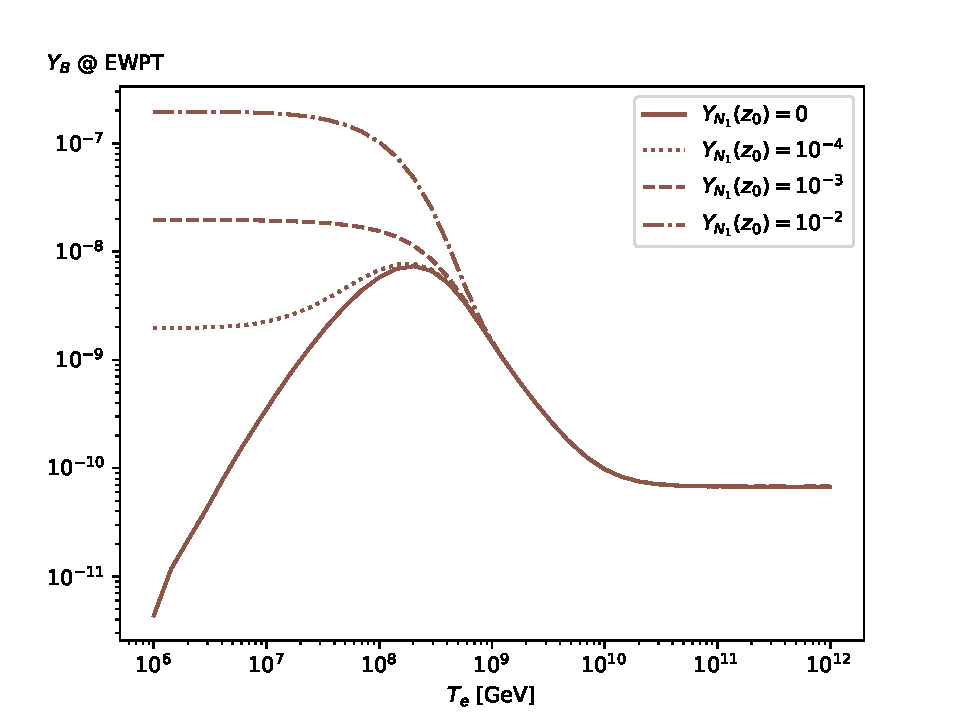
\includegraphics[width=13cm]{fig-B-anisotropic.pdf}
	\caption{تغییرات {\footnotesize$Y_{B}$} در گذار فاز الکتروضعیف بر حسب {\footnotesize$T_e$} \label{fig:YB-anisotropic}}
\end{figure}

\chapter{جمع‌بندی}
\label{chap:conclusion}
در این مطالعه، بعد از مروری بر فیزیک نوترینو، بر لپتون‌زایی به مثابه یک رهیافت توجیه عدم تقارن باریونی و به مشکلات آن پرداختیم. یکی از مشکلات اساسی آن نیاز به جرم‌های بسیار بالا برای نوترینوی راست دست است. با توجه به بیان لپتون‌زایی گرمایی در کیهان‌شناسی‌های غیر استاندارد تلاش کردیم تا جرم مورد نیاز برای نوترینوی راست دست را کاهش دهیم. دو مدل کیهان‌شناسی جایگزین مورد نظر ما، کیهان‌شناسی نافزونور و ناهمسانگرد است؛ که بترتیب در اثر تعمیم مکانیک آماری حاکم بر عالم و صرف نظر کردن از اصل کیهان‌شناختی همسانگردی در بزرگ مقیاس حاصل می‌گردند.

در کیهان‌شناسی نافزونور نشان دادیم عدم تقارن تولید شده با توجه به تغییر پیدا کردن مقادیر تعادلی ذرات و پارامترهای واپاشی و شستشو می‌تواند تحت تاثیر قرار گیرد. در واقع متوجه شدیم برای حالت {\footnotesize$q<1$} پارامتر شستشو ضعیف‌تر است، بنابراین نقض \lr{\footnotesize CP} با شدت بیشتری می‌تواند رخ داده و عدم تقارن را افزایش دهد. نتایج عددی نیز نشان دادند این استدلال صحیح بوده و عدم تقارن در این حالت افزایش می‌یابد. در نهایت تاکید می‌کنیم که می‌توان با در نظر گرفتن حالت {\footnotesize$q<1$} برخلاف حالت {\footnotesize$q>1$}، جرم نوترینوی راست دست را کاهش داد.

در کیهان‌شناسی ناهمسانگرد نشان دادیم عدم تقارن تولید شده با توجه به تغییر پیدا کردن پارامترهای واپاشی و شستشو می‌تواند تحت تاثیر قرار گیرد. در واقع با حل عددی معادلات تحول حاکم نشان دادیم که به ازای ناهمسانگردی خاص می‌تواند عدم تقارن را نسبت به حالت استاندارد افزایش دهد. لذا می‌توان عنوان کرد ناهمسانگردی می‌تواند جرم نوترینوی راست دست مورد نیاز برای لپتون‌زایی را کاهش دهد.

در ادامه این مسیر، می‌توان تاثیر کیهان‌شناسی‌های غیر استاندارد دیگر را بر سناریو‌های باریون‌زایی و بخصوص لپتون‌زایی گرمایی و تعمیم‌های آن مطالعه کرد.

\appendix
\chapter{مباحثی از نظریه‌ی میدان کوانتومی}
\label{appendix:QFT}
در این پیوست به مرور برخی مباحث نظریه میدان کوانتومی که مورد استفاده ما در این پایان‌نامه است، می‌پردازیم.
\section{قوائد فاینمن برای میدان‌های نرده‌ای و فرمیون دیراک}
\label{appendix:Dirac}
قوائد فاینمن متداول برای فرمیون‌های در متون کتب درسی نظریه میدان نظیر  \cite{Peskin:1995ev,Schwartz:2014sze} به تفصیل بررسی می‌شوند و در اینجا فقط من باب مرور آنها را ذکر می‌کنیم. برای انتشارگرهای میدان‌های نرده‌ای و فرمیون دیراکی بترتیب داریم،
\par
\vspace{-0.5cm}
{\footnotesize\begin{equation}
	\label{eq:scaler-propagator}
	\parbox{25mm}{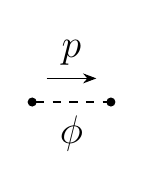
\begin{tikzpicture}
		\begin{feynman}[small]
			\node [dot](a);
			\node [dot,right=of a](b);
			
			\diagram* {
				(a) -- [scalar,edge label'=\(\phi\),momentum=\(p\)] (b),
			};
		\end{feynman}
	\end{tikzpicture}}
	=\frac{-i}{p^2-m_{\phi}^2+i\epsilon},
\end{equation}}
{\footnotesize\begin{equation}
	\label{eq:dirac-propagator}
	\parbox{25mm}{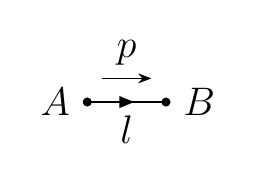
\begin{tikzpicture}
			\begin{feynman}[small]
				\node [dot,label=180:\(A\)](a);
				\node [dot,label=0:\(B\),right=of a](b);
				
				\diagram* {
					(a) -- [fermion,edge label'=\(l\),momentum=\(p\)] (b),
				};
			\end{feynman}
	\end{tikzpicture}}
	=\left[\frac{-i\left(\slashed{p}+m_l\right)}{p^2-m_{l}^2+i\epsilon}\right]_{AB}.
\end{equation}}
که در آن {\footnotesize$A$} و {\footnotesize$B$} اندیس‌های اسپینور و {\footnotesize$p$} چهار تکانه و {\footnotesize$m$} جرم متناظرشان است. برای خطوط خارجی ورودی و خروجی میدان‌های نرده‌ای، فرمیون و پادفرمیون دیراکی نیز بترتیب داریم،
\par
\vspace{-0.5cm}
{\footnotesize\begin{equation}
	\label{eq:scalar-incoming}
	\parbox{25mm}{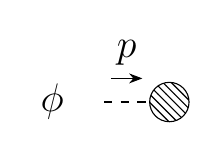
\begin{tikzpicture}
			\begin{feynman}[small]
				\node [label=180:\(\phi\)](a);
				\node [blob,right=of a](b);
				
				\diagram* {
					(a) -- [scalar,momentum=\(p\)] (b),
				};
			\end{feynman}
	\end{tikzpicture}}
	=1, \quad
\end{equation}}
{\footnotesize\begin{equation}
	\label{eq:scalar-outgoing}
	\parbox{25mm}{\begin{tikzpicture}
			\begin{feynman}[small]
				\node [blob,right=of a](a);
				\node [label=180:\(\phi\)](b);
				
				\diagram* {
					(a) -- [scalar,momentum=\(p\)] (b),
				};
			\end{feynman}
	\end{tikzpicture}}
	=1,
\end{equation}}
{\footnotesize\begin{equation}
	\label{eq:fermion-incoming}
	\parbox{25mm}{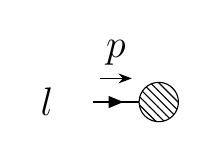
\begin{tikzpicture}
			\begin{feynman}[small]
				\node [label=180:\(l\)](a);
				\node [blob,right=of a](b);
				
				\diagram* {
					(a) -- [fermion,momentum=\(p\)] (b),
				};
			\end{feynman}
	\end{tikzpicture}}
	=u(p),
\end{equation}}
{\footnotesize\begin{equation}
	\label{eq:fermion-outgoing}
	\parbox{25mm}{\begin{tikzpicture}
			\begin{feynman}[small]
				\node [blob,right=of a](a);
				\node [label=180:\(l\)](b);
				
				\diagram* {
					(a) -- [fermion,momentum=\(p\)] (b),
				};
			\end{feynman}
	\end{tikzpicture}}
	=\overline{u}(p),
\end{equation}}
{\footnotesize\begin{equation}
	\label{eq:anti-fermion-incoming}
	\parbox{25mm}{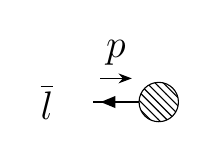
\begin{tikzpicture}
			\begin{feynman}[small]
				\node [label=180:\(\overline{l}\)](a);
				\node [blob,right=of a](b);
				
				\diagram* {
					(a) -- [anti fermion,momentum=\(p\)] (b),
				};
			\end{feynman}
	\end{tikzpicture}}
	=\overline{v}(p),
\end{equation}}
{\footnotesize\begin{equation}
	\label{eq:anti-fermion-outgoing}
	\parbox{25mm}{\begin{tikzpicture}
			\begin{feynman}[small]
				\node [blob,right=of a](a);
				\node [label=180:\(\overline{l}\)](b);
				
				\diagram* {
					(a) -- [anti fermion,momentum=\(p\)] (b),
				};
			\end{feynman}
	\end{tikzpicture}}
	=v(p).
\end{equation}}

\section{قوائد فاینمن برای فرمیون‌های مایورانا}
\label{appendix:Majorana}
وقتی در مورد نوترینوی مایورانا صحبت می‌کنیم، باید در حساب نمودارهای فاینمن، قوائد متناظر آن را بکار ببندیم. لذا در این قسمت به استخراج قوائد فاینمن فرمیون‌های مایورانا با رهیافت مرجع \cite{Luty:1992un} می‌پردازیم که بسادگی امکان‌پذیر است.
\subsection{انتشارگر فرمیون مایورانا}
برای شروع، بخش جنبشی و جرمی لاگرانژی نوترینوی راست دست، {\footnotesize$\nu_R = (\nu_{1R}, \nu_{2R}, \nu_{3R})^T$} که در آن زیروندها مربوط به اندیس در فضای طعم است، را می‌نویسیم
\par
\vspace{-0.5cm}
{\footnotesize\begin{align}
	\mathcal{L}^{R} = i \overline{\nu}_R \slashed{\partial} \nu_R - \frac{1}{2} \overline{\nu}_R^C M^R \nu_R - \frac{1}{2} \overline{\nu}_R (M^R)^* \nu_R^C.
\end{align}}
برای قطری کردن {\footnotesize$M^R$}، با تعریف یک ماتریس یکانی، {\footnotesize$V$} بطوری که {\footnotesize$\nu_R= V^{\dagger} N_R$} برقرار باشد، می‌توان لاگرانژی را بصورت
\par
\vspace{-0.5cm}
{\footnotesize\begin{align}
	\mathcal{L}^{R} =  i \overline{N}_R \slashed{\partial} N_R - \frac{1}{2} \overline{N}_R^C D_M N_R - \frac{1}{2} \overline{N}_R D_M N_R^C,
\end{align}}
نوشت که در آن {\footnotesize$D_M$} ماتریس قطری جرمی نوترینوهای راست دست است.
حال با توجه به معرفی میدان مایورانای چهار مولفه‌ای {\footnotesize$N_k \equiv N_{kR}+N_{kR}^C$} که در شرط مایورانا (\ref{eq:majorana-cond}) صدق می‌کند، می‌توان لاگرانژی را بصورت
\par
\vspace{-0.5cm}
{\footnotesize\begin{align}
	\mathcal{L}^{R} &= \overline{N}_{k} \left(i \slashed{\partial}- M_k\right) N_{k}\notag\\
	&= -N^T_{k} C^{\dagger} \left(i \slashed{\partial}- M_k\right) N_{k},
\end{align}}
بازنویسی کرد. حال با قیاس لاگرانژی دیراک و انتشارگر فرمیون دیراکی، انتشارگر فرمیون مایورانا را می‌توان بصورت
{\footnotesize\begin{equation}
	\label{eq:majorana-propagator}
	\parbox{25mm}{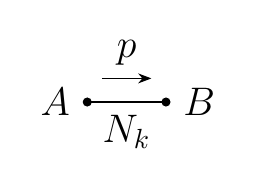
\begin{tikzpicture}
			\begin{feynman}[small]
				\node [dot,label=180:\(A\)](a);
				\node [dot,label=0:\(B\),right=of a](b);
				
				\diagram* {
					(a) -- [edge label'=\(N_k\),momentum=\(p\)] (b),
				};
			\end{feynman}
	\end{tikzpicture}}
	=\left[\frac{-i\left(\slashed{p}+M_k\right)C}{p^2-M_k^2+i\epsilon}\right]_{AB},
\end{equation}}
نوشت؛ که در آن {\footnotesize$A$} و {\footnotesize$B$} اندیس‌های اسپینور و {\footnotesize$p$} چهار تکانه است.
								
\subsection{ضرایب رئوس شامل فرمیون مایورانا}
در بحث ما تنها یک اندرکنش برای نوترینوی راست دست وجود دارد که ناشی از جفت شدگی یوکاوا است که بصورت معادله‌ی (\ref{eq:yukawa}) بیان می‌شود.
حال با استفاده از ماتریس یکانی {\footnotesize$V$} که رابطه‌ی {\footnotesize$\nu_R= V^{\dagger} N_R$} را ارضا کند، ‌‌‌‌می‌توان لاگرانژی اخیر را در ویژه‌پایه‌های جرمی نوترینوهای راست دست نوشت،
\par
\vspace{-0.5cm}
{\footnotesize\begin{align}
		\mathcal{L}^{\rm Yukawa}=-y \overline{l}_L \phi N_R + \rm H.c.,
		\label{eq:Yukawa-mass-bases}
\end{align}}
که در آن {\footnotesize$y=Y V^{\dagger}$} است. 
حال می‌توان با توجه به شرط مایورانا (\ref{eq:majorana-cond}) و اندیس گذاری، لاگرانژی را بصورت
{\footnotesize\begin{align}
	\mathcal{L}^{\rm Yukawa}&= y_{jk} \overline{l}_{L_j} \phi P_R N_k  - y^*_{jk} \overline{N}_k \phi^{\dagger} P_L l_{L_j} ,\notag\\
	&=-y_{jk} \overline{l}_{L_j}\phi  P_R N_k + y^*_{jk} N_k^T C^{\dagger} \phi^{\dagger} P_L l_{L_j}.
\end{align}}
نوشت. بنابراین با توجه به عبارت بدست آمده می‌توان ضرایب رئوس دو فرآیند را بصورت
{\footnotesize\begin{equation}
	\label{eq:majorana-vertex-factor-lepton}
	\parbox{35mm}{\begin{tikzpicture}
			\begin{feynman}[small]
				\vertex [label=180:\(N_k\)](a);
				\vertex [right=of a](b);
				\vertex [label=0:\(\overline{\phi}\),above right= of b](c);
				\vertex [label=0:\(l_{L_j}\),below right=of b](d);
				
				\diagram* {
					(a) -- (b),
					(b) -- [scalar] (c),
					(b) -- [fermion] (d),
				};
			\end{feynman}
	\end{tikzpicture}}
	=-iy_{jk} P_R,
\end{equation}}
{\footnotesize\begin{equation}
	\label{eq:majorana-vertex-factor-anti-lepton}
	\parbox{35mm}{\begin{tikzpicture}
			\begin{feynman}[small]
				\vertex [label=180:\(N_k\)](a);
				\vertex [right=of a](b);
				\vertex [label=0:\(\phi\),above right= of b](c);
				\vertex [label=0:\(\overline{l}_{L_j}\),below right=of b](d);
				
				\diagram* {
					(a) -- (b),
					(b) -- [scalar] (c),
					(b) -- [anti fermion] (d),
				};
			\end{feynman}
	\end{tikzpicture}}
	=-iy^*_{jk} C^{\dagger} P_L,
\end{equation}}
بیان کرد.
\subsection{خطوط خارجی فرمیون مایورانا}
با توجه به شرط مایورانا (\ref{eq:majorana-cond}) تنها اختلاف خطوط خارجی با فرمیون دیراک در مزدوج گیری آنها است. بنابراین،
{\footnotesize\begin{equation}
	\label{eq:majorana-incoming}
	\parbox{25mm}{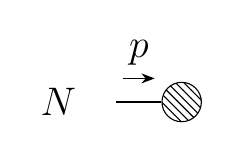
\begin{tikzpicture}
			\begin{feynman}[small]
				\node [label=180:\(N\)](a);
				\node [blob,right=of a](b);
				
				\diagram* {
					(a) -- [momentum=\(p\)] (b),
				};
			\end{feynman}
	\end{tikzpicture}}
	=u^c(p),
\end{equation}}
{\footnotesize\begin{equation}
	\label{eq:majorana-outgoing}
	\parbox{25mm}{\begin{tikzpicture}
			\begin{feynman}[small]
				\node [blob,right=of a](a);
				\node [label=180:\(N\)](b);
				
				\diagram* {
					(a) -- [momentum=\(p\)] (b),
				};
			\end{feynman}
	\end{tikzpicture}}
	=u(p).
\end{equation}}

\bibliographystyle{JHEP}
\lr{\footnotesize\bibliography{biblio}}
\addcontentsline{toc}{chapter}{مراجع}

\includepdf[pages={8-1}]{english.pdf}

\end{document}